\documentclass[12pt]{report}
\usepackage[italian]{babel}
\usepackage{amsmath}
\usepackage{amsthm}
\usepackage[most]{tcolorbox}
\usepackage{tabularx}
\usepackage{amssymb}
\usepackage{enumitem}
\usepackage{amsfonts}
\usepackage{centernot}
\usepackage{wrapfig}
\usepackage{circuitikz}
\usepackage{float}
\usepackage{multirow}
\usepackage{karnaugh-map}
\usepackage{lmodern}
\usepackage{hyperref}
\usepackage{mathtools}
\usepackage{relsize}
\usepackage{mathrsfs}
\usepackage{bm}
\usepackage{xfrac}
\usepackage{lipsum}
\usepackage{bbm}
\usepackage{tikz}
\usepackage{cancel}
\usepackage{mathtools}
\usepackage{multicol}
\usepackage{makecell}
\usepackage{listings}
\usepackage{xcolor}
\usepackage{pgfplots}
\usepackage{calligra}
\usepackage[toc,page]{appendix}
\usepackage{tikz}
\usepackage{yhmath}
\usetikzlibrary{angles, quotes, patterns}
\usepackage{circledsteps}
\setlist[enumerate]{label*=\arabic*.}
\usepackage{bbm}
\title{Architettura degli elaboratori}
\date{}
\setcounter{chapter}{0}
\setlist[enumerate]{label*=\arabic*.}
\setlength{\parindent}{0pt}
\definecolor{brickred}{RGB}{182, 50, 28}
\definecolor{darkred}{RGB}{139, 0, 0}
\hypersetup{
	colorlinks=true,
	linkcolor=darkred,
	filecolor=darkred,
	urlcolor=darkred
}
\newcounter{theorem}
\newcounter{lemma}
\newcounter{corollary}
\newcounter{definition}
\newcounter{exercise}


\labelformat{theorem}{teorema #1}
\labelformat{lemma}{lemma #1}
\labelformat{corollary}{corollario #1}
\labelformat{definition}{definizione #1}
\labelformat{note}{nota #1}
\labelformat{example}{esempio #1}
\labelformat{exercise}{esercizio #1}

\newtcbtheorem[number within=chapter,use counter=theorem]{theorem}%
{Teorema}{arc=1mm,outer arc=1mm,colframe=cyan!55!black,fonttitle=\scshape,lefttitle=1mm,separator sign dash,description font=\bfseries,description delimiters={\flqq}{\frqq}}{th}

\newtcbtheorem[number within=theorem,use counter=corollary]{corollary}%
{Corollario}{arc=1mm,outer arc=1mm,colframe=cyan!55!black,fonttitle=\scshape,lefttitle=1mm,separator sign dash,description font=\bfseries,description delimiters={\flqq}{\frqq}}{cor}

\newtcbtheorem[number within=chapter,use counter=lemma]{lemma}%
{Lemma}{arc=1mm,outer arc=1mm,colframe=cyan!55!black,fonttitle=\scshape,lefttitle=1mm,separator sign dash,description font=\bfseries,description delimiters={\flqq}{\frqq}}{lem}

\newtcbtheorem[number within=chapter,use counter=definition]{definition}%
{Definizione}{breakable, enhanced, arc=1mm,outer arc=1mm,colframe=green!55!black,fonttitle=\scshape,separator sign dash,description font=\bfseries,description delimiters={\flqq}{\frqq}}{def}

\newtcbtheorem[no counter]
{note}{Nota}{blanker,breakable,left=5mm,before skip=10pt,after skip=10pt,borderline west={2.5mm}{0pt}{red!55},coltitle=black,fonttitle=\bfseries}{note}

\newtcbtheorem[no counter]
{example}{Esempio}{blanker,breakable,left=5mm,before skip=10pt,after skip=10pt,borderline west={2.5mm}{0pt}{yellow!55},coltitle=black,fonttitle=\bfseries}{exa}

\newtcbtheorem[number within=section,use counter=exercise]
{exercise}{Esercizio}{blanker,breakable,left=5mm,before skip=10pt,after skip=10pt,borderline west={2.5mm}{0pt}{yellow!55},coltitle=black,fonttitle=\bfseries}{exe}

\newtcbtheorem[no counter]
{assignment}{Traccia}{blanker,breakable,left=5mm,before skip=10pt,after skip=10pt,borderline west={2.5mm}{0pt}{brickred!65},coltitle=black,fonttitle=\bfseries}{asg}

\tcolorboxenvironment{proof}{blanker,breakable,left=5mm,before skip=10pt,after skip=10pt,borderline west={2.5mm}{0pt}{cyan!55!black}}
\newcommand{\namerefl}[1]{%
	\bgroup
	\let\nmu\MakeLowercase
	\nameref{#1}\egroup}

\newcommand{\nmu}{}

\begin{document}
	{
	\let\cleardoublepage\clearpage
	\maketitle
	\tableofcontents
	}
	\chapter{I calcolatori}
	\section{Introduzione e caratteristiche dei calcolatori, legge di Moore, tipologie di computer}
		Un calcolatore è una macchina in grado di svolgere dei compiti per le persone eseguendo le istruzioni che le vengono assegnate. \\ 
		L'industria del computer avanza più velocemente di tutte le altre. Il principale cavalo di battaglia è la capacità di integrare giorno dopo giorno sempre più transistor all'interno dei chip. Avere più transistor significa avere memorie più grande e processori più potenti.
		\begin{tcolorbox}[colframe=blue!75!black, colback=white!5!white, title=Legge di Moore, fonttitle=\bfseries]	
			La legge di Moore afferma che il numero dei transistor in un chip raddoppia ogni 18 mesi, infatti si è passati ad avere un numero di 1000 transistor negli anni '60 ad averne 50 miliardi nel 2020.
		\end{tcolorbox} 
		La crescita in numero dei transistor in un chip comporta ad avere transistor sempre più piccoli e questo è un problema quando il loro spessore sarà di pochi atomi e saranno così piccoli per essere affidabili. \\
		La legge di Moore ha creato un \textbf{circolo virtuoso} perchè gli avanzamenti tecnologici portano a prodotti migliori e più economici che portano alla creazione di nuove applicazioni che creano nuovi mercati e fanno sorgere nuove società. Queste generano competizione che crea la domanda economica per avere tecnologie migliori grazie a cui sconfiggere la concorrenza. \\
		Un altro fattore che guida lo sviluppo tecnologico è la \textbf{legge del software di Nathan} che afferma che: "Il software è come un gas. Si espande fino a riempire il recipiente in cui è contenuto" e quindi, se il software continua ad acquisire sempre più funzionalità questo porta alla richiesta di processori sempre più veloci, memorie più grandi e supporti di I/O di maggiore capacità
		\\
		Anche i costi di computazione, cioè i calcoli per eseguire le operazioni di calcolo della CPU, hanno subito un notevole decremento, si è passati, infatti, da un costo di 130 trilioni di dollari ad un costo di un decimo di dollaro.
		\\
		\textbf{Nota: }Questo non significa che i chip con un costo computazionale così basso sono le più performanti, sono solo le più economiche in termini di costi computazionali.
		Il calcolatore ha due peculiarità:
		\begin{enumerate}
			\item \textbf{programmabilità: }capacità di specializzare il dispositivo per attività complesse di elaborazione dell'informazione;
			\item \textbf{evoluzione del settore: }non può essere usato in modo consapevole ed informato da chi non conosce i principi generali di funzionamento, questo serve a:
			\begin{itemize}
				\item utilizzarlo correttamente
				\item comprendere le differenze architetturali;
				\item decidere se è in grado di risolvere una classe di problemi appartenenti al dominio d'uso, quindi se è adatto al nostro scopo e se è in grado di fornirci i risultati desiderati in un tempo certo.
			\end{itemize}
		\end{enumerate}
		Sul mercato sono presenti diverse tipologie di computer:
		\begin{itemize}
			\item \textbf{Usa e getta}: Questi sono i chip inseriti all'interno delle cartoline di auguri ad esempio, che emettono la melodia. Il più importante sviluppo nell'area di questi tipi di computer è rappresentato dai chip \textbf{RFID}.
			\item \textbf{Microcontrollori}
			\item Supercomputer;
			\item Mainframe e min;
			\item Personal Computer;
			\item Server;
			\item Workstation;
			\item Notebook;
			\item Palmari.
		\end{itemize}
		\section{Sviluppo del computer}
		\subsection{Generazione zero - Computer meccanici}
		La prima persona che costruì una macchina calcolatrice funzionante fu lo scienziato Blaise Pascal che costruì questo dispositivo nel 1642 per aiutare suo padre. La macchina era completamente meccanica, costituita da ingranaggi e azionata a mano con una manovella ed era in grado solo di eseguire somme e sottrazioni. \\
		30 anni dopo, un matematico tedesco, Leibniz, costruì un'altra macchina capace di eseguire anche moltiplicazioni e divisioni. \\
		Circa 150 anni dopo, il matematico Babbage, costruì la \textbf{different engine} e fu progettato per calcolare tabelle di numeri utili per la navigazione. Questa macchina venne costruita per eseguire un solo algoritmo, il metodo matematico delle differenze finite. Un aspetto interessante di questa macchina era l'output che veniva inciso tramite una punta d'acciaio su una lastra di rame. \\
		Dopodichè, Babbage costruì la \textbf{analytical engine} che era composta dal magazzino (la memoria), dal mulino (l'unità computazionale), il dispositivo di input (le schede perforate) e il dispositivo di output (output stampato e perforato). \\
		Il grande avanzamento di questa macchina era rappresentato dal fatto che era di uso generale, leggeva le istruzioni dalle schede perforate e le eseguiva. \\
		Visto che questa macchina era programmabile tramite un linguaggio assemblativo era necessario produrre il software e Babbage assunse Ada Augusta Lovelace che fu la prima programmatrice della storia e in suo onore fu chiamato il linguaggio di programmazione Ada. \\
		Nonostante le macchina di Babbage non erano prive di errori, le sue idee erano in largo anticipo sui tempi, tanto da considerarlo il nonno dei calcolatori moderni. \\
		Un significativo avanzamento avvenne verso la fine degli anni '30, quando uno studente di ingegneria tedesco, Zuse, costruì una serie di macchina calcolatrici automatiche utilizzando relé elettromagnetici, ma le sue macchina vennero distrutte in guerra durante un bombardamento. \\
		Poco tempo dopo, due ricercatori statunitensi Atanasoff e Stibbitz si dedicarono alla progettazione di calcolatori. La macchina di Atansoff era molto avanzata, era basata sull'aritmetica binaria e utilizzava dei condensatori per la memoria così la memoria veniva periodicamente aggiornata, però questa macchina non divenne mai operativa. \\
		Il computer di Stibbitz, invece, era meno evoluto di quello di Atansoff e riuscì a funzionare. \\
		Dopodichè uno studente universitario, Aiken, che svolgeva a mano complessi calcoli numerici, capì l'importanza di poter svolgere calcoli per mezzo di una macchina, e dopo aver studiato le macchina dei suoi predecessori sviluppò la \textbf{Mark I} che era la macchina di uso generale di Babbage costruita, però, per mezzo dei relé elettronici, più tardi realizzò la \textbf{Mark II} e iniziò l'era dell'elettronica.
		\subsection{Prima generazione - Valvole}
		Lo stimolo per lo sviluppo dei computer venne dalla Seconda Guerra Mondiale quando i britannici intercettavano i messaggi mandati via radio dagli ammirati tedeschi ai sottomarini. Questi messaggi venivano codificato per mezzo dell'\textbf{ENIGMA} sviluppato da Thomas Jefferson. \\
		Tuttavia codificare un messaggio richiedeva molto tempo, ed era necessario farlo velocemente, per questo il governo britannico costruì un computer chiamato COLOSSUS, grazie anche all'aiuto di Alan Turing, e questo fu il primo elaboratore digitale al mondo. \\
		Più tardi del 1943 venne progettato il computer \textbf{ENIAC} che era dotata di 20 registri, ciascuno dei quali in grado di memorizzare un numero decimale a 10 cifre. ENIAC veniva programmato regolando 6000 interruttori multi-posizione e connettendo molte prese con una foresta di cavi. \\
		La macchina fu completata nel 1946, quando ormai non era più utile per lo scopo originario. \\
		Più tardi iniziò la progettazione del suo successore, l'\textbf{EDVAC} e durante la lavorazione, un membro del progetto ENIAC, John Von Neumann, costruì la sui versione dell'EDVAC, la macchina \textbf{IAS}, il quale sviluppò il progetto della \textbf{macchina di Von Neumann}.
		\subsection{Seconda generazione - Transisor}
		Il transistor è stato inventato nel 1948 e in 10 anni essi rivoluzionarono i computer tando da rendere i computer a valvole obsoleti. \\
		Il primo computer a transistor era il \textbf{TX-0} ideato semplicemente per testare il TX-2 che però non fu mai progettato. \\
		Più tardi apparve la macchina \textbf{PDP-1} con 4096 parole di 18 bit e in grado di eseguire 200.000 istruzioni al secondo, prestazioni che corrispondevano alla metà dell'\textbf{IBM 7090} che era il calcolatore più veloce dell'epoca. \\
		Un'innovazione del PDP-1 era dovuto dal fatto che era costituito da un display visuale e dalla capacità di disegnare punti in qualsiasi zona dello schermo. Pochi anni dopo venne introdotto il modello \textbf{PDP-8} più economica in quanto aveva un unico bus, l'\textbf{omnibus}. \\
		IBM, come già anticipato, sviluppò i modelli \textbf{7090} e \textbf{7094} e grazie ad essi IBM divenne una delle principali forze del mercato, otteneva grandi profitti vendendo alle aziende il modello \textbf{1401} che aveva una velocità paragonabile al 7094. \\
		Nel 1964 una sconosciuta società, la Control Data Corporation, introdusse il modello \textbf{6600} più veloce del 7094 di IBM, in quanto la CPU era una macchina altamente parallela e inoltre al suo interno aveva un certo numero di piccoli computer che lo aiutavano. Il progettista di questo modello, \textbf{Seymour Cray} dedicò la sua vita a sviluppare macchine sempre più veloci, i \textbf{supercomputer}
		\subsection{Terza generazione - Circuiti integrati}
		Nel 1958 l'invenzione dei circuiti integrati su silicio di Robert Noyce permise di realizzare su un unico chip decide di transistor. Questo metodo di assemblaggio rese possibile la costruzione di computer sempre più piccoli, veloci ed economici. \\
		L'IBM introdusse una famiglia di computer, il \textbf{System/360}, basata su circuiti integrati e in grado di svolgere calcoli scientifici e commerciali. In una famiglia di computer, il software scritto per un modello più piccolo poteva essere tranquillamente eseguito su un modello più grande. \\
		Una caratteristica importante del 360 era lo spazio di indirizzi pari a $2^24$ che all'epoca appariva come una quantità di memoria infinita
		Un'altra innovazione fu la \textbf{multiprogrammazione} grazie a cui è possibile avere più programmi in memoria allo stesso tempo.
		\subsection{Quarta generazione - Integrazione a grandissima scala}	
		Negli anni '80 la tecnologia \textbf{VLSI} permise di inserire in un unico chip un numero sempre maggiore di transistor, fino ad arrivare a milioni di transistor. e questo portò allo sviluppo di computer sempre più piccoli e veloci, perchè prima per poter far funzionare i computer bisognava disporre di \textbf{centri di calcolo}, mentre con questa tecnologia ognuno poteva disporre del proprio calcolatore, dando via all'epoca dei \textbf{personal computer}. Successivamente si diffuse per i processori 8080 il sistema operativo \textbf{CP/M} che aveva un file system e una serie di istruzioni che l'utente doveva scrivere con la tastiera per farle leggere da un interprete di comandi. \\
		Un altro dei primi PC fu \textbf{Apple}. \\
		Nel 1981 venne introdotto il \textbf{PC IBM} costruito solo di componenti commerciali e divenne il computer più venduto della storia ed era in grado di schiacciare tutti gli altri. \\
		L'unico sopravvissuto era il Macintosh di Apple, primo computer dotato di una \textbf{GUI}. \\
		In questo periodo vennero sviluppati i primi PC portatili e l'Intel sviluppò CPU migliori e più potenti e vennero sviluppati i sistemi operativi \textbf{MS-DOS} e \textbf{Windows}.
		\subsection{Quinta generazione - Computer invisibili}
		Nel 1981 il governo giapponese voleva stanziare molto denaro per sviluppare una nuova generazione di computer basata sull'intelligenza artificiale, però questo progetto fallì e venne abbandonato. \\
		Quella che può essere definita quinta generazione è la riduzione in termini di dimensione dei computer. Un'altra caratteristica di questa generazione sono i computer invisibili, poichè integrati in elettrodomestici, orologi, carte di credito e molto altro.
		\section{Architettura di Von Neumann e le sue componenti}
		L'architettura del moderno microcomputer ha radici che risalgono ai primi anni 040 e il matematico John Von Neumann ha sviluppato un modello di computer che viene utilizzato ancora oggi per descrivere gli elaboratori.
		L'architettura di Von Neumann è composta da:
		\begin{itemize}
			\item \textbf{RAM: }la memoria centrale, che memorizza data e programmi;
			\item \textbf{CPU: }la parte centrale, composta dal processore, considerata il "cervello" del computer, composta dall'\textbf{ALU} che compie calcoli di tipo aritmetico e di tipo logico e l'\textbf{unità di controllo} che esegue i programmi;
			\item \textbf{Dispositivi di Input: }tramite i quali i dati vengono inseriti nel calcolatore per essere elaborati;
			\item \textbf{Dispositivi di Output: }tramite i quali i dati vengono trasmessi all'utente;
			\item \textbf{BUS: }un canale di trasmissione che collega tutte le componenti fra loro;
		\end{itemize}
		La \textbf{RAM}, \textbf{R}andom \textbf{A}ccess \textbf{M}emory, è una memoria ad accesso casuale, cioè a seconda della cella che occupa il dato in memoria, la RAM accede ad esso nello stesso tempo.
		\\
		La RAM è anche una memoria di tipo volatile, cioè, conservano il dato solo in presenza di corrente elettrica, in caso contrario il dato viene perso.
		\section{Linguaggi di programmazione}
		L'elaboratore esegue i programmi, che è una sequenza di istruzioni macchina comprensibili dal calcolatore e tramite sequenze diverse di istruzioni e con dati diversi il calcolatore esegue cose diverse.
		\\
		\textbf{L0:} Linguaggio macchina
		\\
		\textbf{L1:} Linguaggio di più alto livello
		\\
		Se gli utenti scrivono un programma in livello L1 e il calcolatore comprende il livello L0, bisogna tradurre le istruzioni da L1 a L0 attraverso due procedimenti: \textbf{traduzione} e \textbf{interpretazione}.
		\\
		Nella traduzione, effettuata dal \textbf{compilatore}, il programma scritto in linguaggio L1 viene interamente convertito in programma L0 e viene caricato nella memoria del computer per poter essere eseguito, mentre nell'interpretazione ciascuna istruzione L1 viene esaminata, decodificata ed eseguita direttamente. Quest'ultima viene eseguita dall'\textbf{interprete}.
		\\
		I programmi scritti in un vero linguaggio macchina possono essere eseguiti direttamente dai circuiti dei computer che formano l'\textbf{hardware} del computer. Al contrario il \textbf{software} consiste di \textbf{algoritmi} e i due, \textbf{\textit{hardware e software, sono logicamente equivalenti}}. \\
		Ogni operazione eseguita via software può anche essere costruita direttamente in hardware ed è vero anche il contrario. \\
		La scelta di collocare certe funzioni nell'hardware piuttosto che nel software dipende da fattori quali costo, velocità, affidabilità e la frequenza di modifiche che ci aspetta.
		\section{Macchine multilivello}
		La maggior parte dei computer moderni consiste di due o più livelli, ad esempio una macchina potrebbe essere formata da 6 livelli.
		\begin{figure}[h]
			\centering
			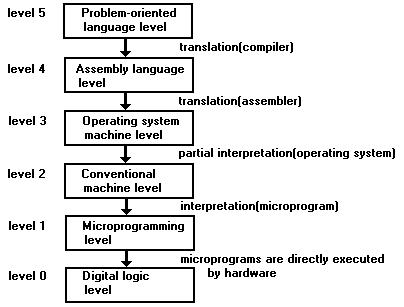
\includegraphics{multilevel_machine}
			\caption{Calcolatore formato da 6 livelli}
			\label{fig:mesh1}
		\end{figure}
		\newpage
		\subsection{Livello 0 - Livello logico digitale}
		Il livello logico, sono le porte logiche, costruite utilizzando componenti analogici, i transistor. Le porte logiche operano sui segnali e possono assumere due stati, 0 o 1.
		\\
		Ogni porta logica esegue una semplice operazione matematica sugli ingressi digitali e produce un'uscita basata su una funzione logica.
		Le operazioni più comuni sono:
		\begin{figure}[H]
			\centering
			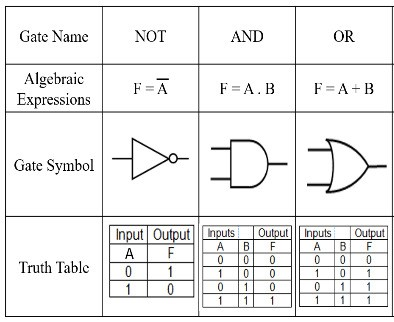
\includegraphics[width=0.75\textwidth]{logic_gates}
			\caption{Porte logiche AND, OR, NOT}
			\label{fig:mesh2}
		\end{figure}
		Queste porte sono alla base di tutti i circuiti digitali e possono essere combinate così da costruire strutture più complesse come memorie o registri.
		\subsection{Livello 1 - microarchitettura}
		Qui vi è una memoria locale, formata da un gruppo di registri e l'\textbf{ALU},
		\\
		I registri sono connessi all'ALU per formare un data path lungo il quale questi ultimi si spostano.
		L'operazione del data path consiste nel:
		\begin{itemize}
			\item Selezionare uno o due registri;
			\item Permettere alla ALU di operare su di loro;
			\item Memorizzare il risultato in uno dei registri.
		\end{itemize}
		In alcune macchine le operazioni sono controllate da un programma chiamato \textbf{microprogramma} mentre su altre è controllato direttamente dall'hardware
		\subsection{Livello 2 - ISA, Livello di microprogrammazione}
		L'\textbf{ISA}, \textbf{I}nstruction \textbf{S}et \textbf{A}rchitecture, definisce l'interfaccia fra il software e l'hardware e rappresenta l'insieme delle operazioni che un processore può eseguire e il modo in cui il software può interagire con il processore.
		\\
		Il livello ISA rappresenta la "visione" che il software ha dell'hardware. Questo livello fornisce il formato delle istruzioni. i registri che sono disponibili per il programmatore e il modo in cui le operazioni di calcolo vengono effettuate.
		Diversi processori utilizzano ISA differenti:
		\begin{itemize}
			\item \textbf{x86} e \textbf{x86-64}: uno degli ISA più diffusi, utilizzato nei PC. L'x86-64 è un'estensione a 64 bit dell'x86. Questo ISA supporta un vasto set di istruzioni, registri estesi e operazioni avanzate di memoria;
			\item \textbf{ARM}: viene utilizzato principalmente nei dispositivi mobili e negli embedded ed è noto per la sua efficienza energetica  e semplicità;
			\item \textbf{RISC-V}: questo ISA è aperto e modulare e offre un set di istruzioni di base che può essere esteso con funzionalità specializzate;
			\item \textbf{MIPS}: presenza un'architettura ISA RISC (Reduced Instruction Set Computer), spesso utilizzata in sistemi embedded e sistemi specializzati.
		\end{itemize}
		\subsection{Livello 3 - Sistema operativo}
		Il sistema operativo è il software che funge da intermediario tra l'utente e l'hardware e tra il software applicativo e l'hardware. 
		Il suo scopo è quello di gestire le risorse del computer e garantire che i vari programmi possano funzionare in modo corretto ed efficiente.
		I livelli 2 e 3 sono interpretati e i livelli successivi sono compilati. \\
		I tre livelli inferiori non sono progettati per essere utilizzati dal programmatore medio, ma concepiti per eseguire interpreti e traduttori necessari come supporto per i livelli più alti. \\
		Gli interpreti e i traduttori sono scritti dai \textbf{programmatori di sistema} che sono specializzati nella progettazione e nell'implementazione di nuove macchine virtuali. \\
		I livelli 4 e superiori sono pensati per i programmatori che devono risolvere problemi applicativi.
		\subsection{Livello 4 - Livello assemblativo}
		Questo livello fornisce ai programmatori un modo per scrivere un programma per livelli 1, 2, 3 in una maniera più semplice.
		\\
		L'\textbf{assembly} definisce una notazione simbolica che è in stretta relazione con i codici in linguaggio macchina. Il codice assembly viene tradotto in linguaggio macchina per mezzo dell'\textbf{assembler}.
		\subsection{Livello 5 - Linguaggio ad alto livello}
		Si utilizza l'assembly solo se esistono vincoli stringenti sui tempi di esecuzione e sull'architettura, altrimenti vengono usati dei linguaggi più vicini al linguaggio naturale, i linguaggi ad alto livello sono intermedi fra il linguaggio macchina e i linguaggi naturali.
		\par\noindent\rule{\textwidth}{0.4pt}
		\\
		Riassumendo, i computer sono progettati come una serie di livelli, ciascuno costruito su quelli che lo precedono. Ciascun livello rappresenta una diversa astrazione, caratterizzata dalla presenza di oggetti e operazioni diversi.
		\chapter{Sistemi numerici e rappresentazione digitale dei segnale}
		\section{Il bit, sistemi numerici e codifica dei dati}
		Le informazioni o i dati provenienti dal mondo esterno vengono \textbf{codificati} in rappresentazione digitale che vengono memorizzati ed elaborati dal calcolatore. La procedura inversa è chiamata \textbf{decodifica}.
		\\
		\\
		Il \textbf{bit}, binary digit, è l'unità elementare dell'informazione e può assumere due valori, 0 o 1 che rappresenta l'alfabeto dei calcolatori.
		\\
		Il bit è l'unità minima di memoria non indirizzabile poichè si legge e scrive in memoria a singoli byte, cioè un gruppo di 8 bit e non a bit.
		\\
		Per poter rappresentare un numero maggiore di dati o informazioni si usano \textbf{sequenze} di bit.
		\\
		Con $n$ bit si possono codificare $\mathbf{2^n}$ stati differenti.
		Dati $n$ stati per trovare il numeri di bit necessari bisogna eseguire: $\log_2(n)$.
		\\
		Una \textbf{word} è una quantità di dati di dimensione fissa che un processore può gestire come un'unica unità durante le operazioni di elaborazione.
		I moderni sistemi memorizzano e manipolano molti bit e byte e quindi c'è la necessità di multipli:
		\begin{itemize}
			\item K, Kilobyte, $10^{3}$B;
			\item M, Megabyte, $10^{6}$B;
			\item G, Gigabyte, $10^{9}$B;
			\item T, Terabyte, $10^{12}$B;
			\item P, Petabyte, $10^{15}$B;
			\item E, Exabyte, $10^{18}$B;
			\item Z, Zetabyte, $10^{21}$B;
			\item Y, Yottabyte, $10^{24}$B;
		\end{itemize}
		Un \textbf{sistema numerico} viene determinato per mezzo di: 
		\begin{itemize}
			\item Un numero limitato di simboli;
			\item Regole per costruire i numeri
				\begin{itemize}
					\item \textbf{Posizionali}, il valore della cifra dipende dalla posizione che assume, come nel sistema binario, ottale, decimale ecc;
					\item \textbf{Non posizionali}, il valore della cifra non dipende dalla posizione nella quale si trova;
				\end{itemize}
			\item Regole che permettono di eseguire le operazioni sui numeri.
		\end{itemize}
		Il sistema numerico viene indicato inserendo il pedice alla cifra che si rappresenta come $(77)_8 \ o \ (1011)_2$.
		\\
		\\
		Le tecniche di \textbf{codifica dei dati} sono tre:
		\begin{enumerate}
			\item \textbf{Modulo e segno:} dove la cifra più significativa rappresenta il segno, 0 per i positivi e 1 per i negativi, con $n$ cifre si possono rappresentare i numeri: $-(2^{n-1}+1) \leq x \leq (2^{n-1} - 1)$, lo $0$ viene rappresentato sia come numero positivo che come numero negativo;
			\item \textbf{Complemento a 1:} poco usato, la rappresentazione in complemento a 1 si ottiene invertendo gli 0 delle parola con gli 1 e viceversa;
			\item \textbf{Complemento a 2:} dove il bit più a sinistra indica il segno. Per trasformare un numero positivo in negativo si codifica il numero in complemento a 1 e si aggiunge 1 al risultato.
			Il complemento a 2 di un numero binario è $2^n-(N)_2$.
			Il campo dei numeri rappresentabili è $-(2^{n-1}) \leq x \leq (2^{n-1} - 1)$, in quanto lo $0$ è positivo;
		\end{enumerate} 
		\section{Rappresentazione digitale dei segnali}
		Una \textbf{grandezza analogica} assume valori continui in un intervallo, cioè può assumere infiniti valori e di conseguenza un segnale analogico è più denso di uno digitale.
		\\
		Una \textbf{grandezza digitale} assume, invece, un valore finito di valori in un intervallo.
		\\
		Affinché un calcolatore possa utilizzare un segnale analogico è necessario che questo venga convertito in segnale digitale seguendo diversi processi:
		\begin{itemize}
			\item \textbf{Campionamento:} questo è il processo di conversione di un segnale tempo-continuo in un segnale tempo-discreto e l'ampiezza del segnale continuo viene considerata in intervalli di tempo regolari;
			\item \textbf{Quantizzazione:} questo è il processo di conversione di un segnale a valori continui in uno a valori discreti e più alto è il numero di bit utilizzati nella quantizzazione minore sarà l'\textbf{errore di quantizzazione} e la distanza media tra il valore campionato e il valore quantizzato sarà minore.
		\end{itemize}
		\begin{theorem}{\nmu Teorema del campionamento di Nyquist Shannon}{nyquist_shannon}
			Dato un segnale, con larghezza di banda $B$ finita e nota, la frequenza minima di campionamento, per poter ricostruire correttamente tale segnale, deve essere pari ad almeno $2B$.
			\\
			Un segnale campionato con frequenza pari a $f_c$ avrà massima frequenza risolvibile a $\dfrac{f_c}{2}$.
		\end{theorem}
		\subsection{Codifica dei caratteri}
		Ciascun carattere alfanumerico, di punteggiatura o di controllo che compone il testo deve essere rappresentato in codice binario.
		\\
		Lo standard utilizzato per rappresentare questi caratteri in codice binario è il codice \textbf{ASCII} che utilizza 8 bit, tra i quali 1 di controllo e quindi permette la rappresentazione di 128 caratteri. Questo codice è stato sviluppato principalmente per lingue anglosassoni.
		\\
		\textbf{UNICODE} è il sistema di codifica che assegna un numero univoco ad ogni carattere per la scrittura di testi, in maniera indipendente dalla lingua, dalla piattaforma informatica e dal programma utilizzato. UNICODE utilizza 16 bit e permette di rappresentare $2^{16}$ caratteri, questo comporta dimensioni di file raddoppiate in confronto ai file che utilizzano come sistema di codifica l'ASCII e non tutti gli editor utilizzano UNICODE.
		\subsection{Codifica dell'audio}
		Il suono è definito come una rapida variazione di pressione, prodotta da una sorgente, in un mezzo elastico e questa variazione produce oscillazioni nelle particelle del mezzo.
		\\
		Le oscillazioni sono spostamenti delle particelle intorno alla posizione di riposo e nella direzione di propagazione del suono. Queste oscillazioni sono chiamate \textbf{onde sonore}.
		\\
		La soglia udibile è fra i 20 e i 20kHz e l'audio viene codificato nel formato WAVE, WAVEform audio file format.
		\\
		Gli algoritmi di compressione dei file audio sono \textbf{MP3} per la codifica della musica e ha un tipo di compressione lossy e sfrutta la conoscenza dei limiti dell'udito umano per ridurre la quantità di informazione da memorizzare.
		\subsection{Codifica delle immagini}
		Consideriamo una griglia formata da righe orizzontali e verticali a distanza costante. Ogni quadratino della griglia prende il nome di \textbf{pixel} e viene codificato in binario utilizzando lo $0$ quando il colore bianco è predominante e $1$ quando il nero è predominante.
		La rappresentazione dell'immagine sarà sempre più fedele all'immagine originario all'aumentare dei pixel.
		\\
		\\
		Esistono due \textbf{modelli di colori}:
		\begin{enumerate}
			\item \textbf{RGB:} questo è un modello di colori di tipo additivo, ogni colore viene prodotto come somma di componenti dei tre colori, Rosso, Verde e Blu e viene utilizzato quando si vogliono mescolare fasci di luce colorata sui monitor ad esempio;
			\item \textbf{CMY:} questo è un modello di colori di tipo sottrattivo, ogni colore viene prodotto come sottrazione dei tre colori Ciano, Magenta e Giallo e i colori generati sono meno luminosi e si usa nel caso in cui si mischiano sostanze colorate che riflettono la luce come inchiostri, tempere ecc.
		\end{enumerate}
		La dimensione dell'immagine è data dal numero di pixel che costituiscono la base per il numero di pixel che costituiscono l'altezza.
		\\
		La profondità dell'immagine è il numero di bit che utilizziamo per rappresentare il colore di un singolo pixel dell'immagine.
		\begin{center}
			Numero di bit per immagine = dimensione $\times$ profondità
		\end{center} 
		Nel caso delle immagini le operazioni di campionamento e quantizzazione si applicano nello spazio (2D) invece che nel tempo e il \textbf{campionamento} consiste nel dividere l'immagine in sottoinsiemi regolari per ognuno dei quali si dovrà prelevare un campione che si considera rappresentativo per tutto il sottoinsieme.
		\\
		La \textbf{quantizzazione} è la codifica del colore associato a ogni pixel, i formati più recenti utilizzano 32 bit, di cui 8 per rappresentare le tre componenti fondamentali RGB, altri 8 per gestire le trasparenze.
		\\
		Algoritmi di compressione delle immagini sono:
		\begin{itemize}
			\item formato \textbf{BITMAP};
			\item formato \textbf{GIF};
			\item formato \textbf{JPEG}.
		\end{itemize}
		\subsection{Codifica di un filmato}
		Per codificare un filmato invece, che è una successione di fotogrammi accompagnato da una sequenza di audio, bisogna codificare ogni immagine del fotogramma e codificare l'audio, per fare ciò però servono tanti bit e quindi la soluzione è quella di codificare solo le differenze fra un fotogramma e l'altro, questo prende il nome di algoritmo \textbf{MPEG}.
		\\
		La dimensione del filmato dipende da almeno cinque fattori:
		\begin{enumerate}
			\item \textbf{Lunghezza del filmato} in secondi;
			\item \textbf{Risoluzione grafica}, più fitta è la griglia per digitalizzare i singoli fotogrammi maggiore sarà la risoluzione;
			\item \textbf{L'ampiezza della 'palette'} di colori utilizzata, una palette ristretta rende i colori troppo poco realistici; 
			\item \textbf{Numero di frame per secondo}, un numero limitato di fotogrammi fa apparire l'immagine poco fluida;
			\item \textbf{Qualità dell'audio}.
		\end{enumerate}
	\chapter{Studio del calcolatore}
\section{Architettura di Von Neumann}
L'architettura del moderno calcolatore segue il modello di Von Neumann che si basa su 5 elementi fondamentali: la CPU, la RAM, i dispositivi I/O e il BUS.\\
\begin{figure}[h]
	\centering
	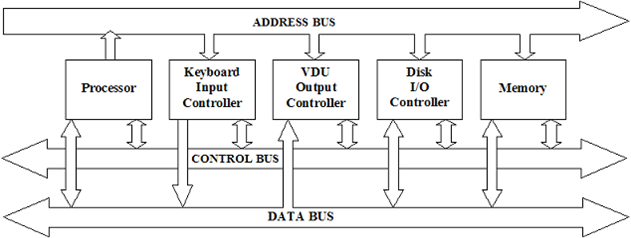
\includegraphics[width=0.75\textwidth]{extended_neumann}
	\caption{La figura mostra una tipica struttura caratterizzata dalla presenza dei tre bus principali}
\end{figure}\\
L'architettura di Von Neumann estesa include altre componenti:
\begin{itemize}
	\item CPU;
	\item ROM;
	\item RAM;
	\item Dispositivi I/O;
	\begin{itemize}
		\item Monitor;
		\item Hard disk;
		\item Drive CD/DVD;
		\item Stampanti;
	\end{itemize}
	\item BUS.
\end{itemize}			
\subsection{Scheda madre}
La scheda madre raccoglie tutta la circuiteria elettronica e i collegamenti di interfaccia fra i vari componenti principali di un calcolatore, fra questi i bus di espansione e le interfacce verso l'esterno ed è responsabile della trasmissione e temporizzazione corretta dei segnali.\\
I principali componenti montati sulla scheda madre sono:
\begin{itemize}
	\item CPU;
	\item RAM;
	\item ROM;
	\item Scheda video e scheda audio.
\end{itemize}
I componenti collegati tramite cavi alla scheda madre sono:
\begin{itemize}
	\item hard disk;
	\item lettore DVD;
	\item alimentatore;
	\item slot lettura penne USB, ecc.
\end{itemize}
\subsection{Oscillatore}
L'oscillatore principale sulla scheda madre, o più semplicemente, \textbf{oscillatore di sistema}, fornisce la frequenza di base per il funzionamento della CPU e di altri dispositivi come il chipset, la RAM o altri componenti.\\
Quest'oscillatore è basato su un cristallo di quarzo che genera il segnale di clock per il sistema. Questo segnale viene inviato alla CPU e ad altri componenti per sincronizzare tutte le operazioni del sistema. \\
\textbf{Moltiplicatore di clock della CPU}: La CPU prende il segnale di clock dalla scheda madre e lo moltiplica internamente per raggiungere la sua frequenza operativa. Questo processo è noto come \textbf{multiplying clock (Phase-Locked Loop (PLL))}. 
\subsection{CPU e i suoi registri}
La CPU è il "cervello" del computer e il suo compito è quello di  eseguire le istruzioni di un programma presente in memoria principale. \\
La CPU è composta da parti distinte:
\begin{itemize}
	\item \textbf{l'unità di controllo:} che si occupa di prelevare le istruzioni dalla memoria principale e determinarne il tipo;
	\item \textbf{l'unità aritmetico-logica:} che esegue le istruzioni come l'addizione e l'AND per portare a termine le esecuzioni delle istruzioni;
	\item \textbf{registri:} costituiscono una memoria ad alta velocità, utilizzata per memorizzare dei risultati temporanei e delle informazioni di controllo e ogni registro ha una funzione diversa e una dimensione predefinita. Il valore complessivo di tutti i registri costituisce lo stato in cui si trova la CPU in un determinato istante.\\
	I registri si suddividono in base al loro scopo:
	\begin{itemize}
		\item Scambio dati con la memoria:
		\begin{itemize}
			\item \textbf{MAR} (Memory Address Register): contiene l'indirizzo di riferimento della memoria;
			\item \textbf{MDR} (Memory Data Register): contiene dati da inviare alla memoria;
		\end{itemize}
		\item Scambio dati con i moduli I/O:
		\begin{itemize}
			\item \textbf{I/O AR} (Input Output Address Register): specifica il dispositivo di I/O;
			\item \textbf{I/O BR} (Input Output Buffer Register): contiene i dati da scambiare con il dispositivo;
		\end{itemize}
		\item Esecuzione delle istruzioni:
		\begin{itemize}
			\item \textbf{Program Counter (PC):} punta all'istruzione successiva che deve essere prelevata per l'esecuzione;
			\item \textbf{Instruction Register (IR):} contiene l'istruzione in fase di esecuzione.
		\end{itemize}
		\item Controllo dell'esecuzione:
		\begin{itemize}
			\item \textbf{PSW}(Program Status Word): contiene delle informazioni di stato
		\end{itemize}
	\end{itemize}
\end{itemize}
\subsection{I BUS}
Un \textbf{bus} è collegamento elettrico che unisce diversi dispositivi. I bus sono classificati in base alla loro funzione; alcuni sono impiegati all'interno della CPU per trasferire dati da e verso l'ALU, mentre altri sono esterni alla CPU e servono a connetterla con la memoria e con altri dispositivi I/O. Ciascun bus soddisfa certi requisiti e gode di proprietà specifiche.
\begin{enumerate}
	\item \textbf{Data Bus:} questo è un insieme di linee di comunicazione utilizzate per trasferire dati tra i diversi componenti di un sistema informatico, come la CPU, la memoria RAM e ROM e dispositivi I/O.\\
	Il data bus presenta diverse \textbf{caratteristiche:}
	\begin{itemize}
		\item \textbf{bidirezionale:} il data bus può trasferire dati in entrambe la direzioni, ad esempio dalla CPU alla memoria e viceversa;
		\item \textbf{larghezza:} la larghezza del bus determina quanti bit di dati possono essere trasferiti simultaneamente. Maggiore è la larghezza maggiori possono essere i bit di dati trasferibili in un solo ciclo di clock;
		\item \textbf{funzione:} quando la CPU esegue un'operazione i dati vengono trasferiti attraverso il data bus.
	\end{itemize}
	\item \textbf{Address Bus:} questo è un insieme di linee di comunicazione utilizzata per specificare gli \textbf{indirizzi di memoria} che la CPU intende leggere o scrivere.
	L'address bus presenta diverse \textbf{caratteristiche}:
	\begin{itemize}
		\item \textbf{unidirezionale:} l'address bus trasferisce informazioni solo dalla CPU verso la memoria o verso i dispositivi I/O, specificando l'indirizzo di memoria che viene utilizzato per un'operazione di lettura o scrittura;
		\item \textbf{larghezza:} la larghezza dell'address bus determina il massimo numero di indirizzi di memoria o di I/O che possono essere utilizzati. Ad esempio un bus di 16 bit può indirizzare $2^{16} = 65.536$ posizioni di memoria, cioè 64Kb;
		\item \textbf{funzione:} ogni volta che la CPU esegue un'operazione di lettura/scrittura, l'indirizzo del dato o del dispositivo coinvolto viene posto sull'address bus, permettendo al sistema di accedere a una specifica locazione di memoria o periferica.
	\end{itemize}
	\item \textbf{Control Bus:} il control bus è un insieme di linee utilizzate per inviare e ricevere \textbf{segnali di controllo} tra la CPU e gli altri componenti del sistema, come la memoria o i dispositivi di I/O. Questi segnali coordinano il flusso dei dati e indicano lo stato delle operazioni.\\
	Le caratteristiche del control bus sono:
	\begin{itemize}
		\item \textbf{bidirezionale:} questo bus è bidirezionale in quanto sia la CPU che i dispositivi esterni possono inviarsi segnali di controllo;
		\item \textbf{Funzione:} come sappiamo il control bus controlla, attraverso dei segnali, il corretto funzionamento delle operazioni, alcuni segnali sono:
		\begin{itemize}
			\item \textbf{Read (RD):} segnala che la CPU desidera leggere dati dalla memoria o dai dispositivi I/O;
			\item \textbf{Write (WR):} indica che la CPU desidera scrivere dati in una locazione di memoria o in un dispositivo I/O;
			\item \textbf{Clock (CLK):} sincronizza tutte le operazioni nel sistema;
			\item \textbf{Interrupt (INT):} permette ai dispositivi esterni di richiedere l'attenzione della CPU;
			\item \textbf{Chip select (CS):} indica a un dispositivo I/O o a una particolare locazione di memoria che deve rispondere alla richiesta di lettura/scrittura.
		\end{itemize}
	\end{itemize}
\end{enumerate}
\section{IPC - Instruction per cycle}
L'\textbf{IPC} indica il numero medio di istruzioni che il processore può completare in un ciclo di clock. \\
Un \textbf{ciclo di clock} è la più piccola unità di tempo in cui un processore può eseguire una parte di operazione. La \textbf{frequenza di clock} misurata in \textbf{Hertz (Hz)}, rappresenta il numero di ciclo di clock che avvengono in un secondo.
\\
I \textbf{MIPS}, invece, misurano il numero di milioni di istruzioni che un processore può eseguire in un secondo.
Ritornando al concetto di IPC, in un mondo ideale, un processore eseguirebbe un'istruzione per ogni ciclo di clock quindi l'IPC sarebbe 1. Tuttavia, a causa di vari fattori, come il tempo di accesso in memoria, la dipendenza tra le istruzioni e la complessità di esse, l'IPC effettivo tende ad essere inferiore a 1, anche se i processori avanzati con pipeline e architetture superscalari possono superare 1 IPC.
\section{Instruction Execution Steps}
La CPU esegue le istruzioni rispettando un specifico algoritmo, chiamato \textbf{ciclo macchina} o \textbf{ciclo fetch-decode-execute}, che si basa su tre operazioni:
\begin{enumerate}
	\item \textbf{instruction fetch:} cioè il recupero di un'istruzione dalla memoria;
	\item \textbf{decode:} cioè l'interpretazione dell'istruzione e l'attivazione delle funzioni associate;
	\item \textbf{execute:} cioè l'esecuzione dell'istruzione e la memorizzazione del risultato.	
\end{enumerate}
I passi che compie la CPU per eseguire un'operazione sono:
\begin{enumerate}
	\item prelevare la successiva istruzione della memoria per portarla nell'IR - \textbf{Fetch};
	\item modificare il PC per farlo puntare all'istruzione seguente - \textbf{Fetch};
	\item  determinare il tipo dell'istruzione prelevata - \textbf{Fetch (decode)};
	\item se l'istruzione usa una parola in memoria, determinare dove si trova - \textbf{Execute};
	\item se necessario, prelevare la parola per portarla in un registro della CPU;
	\item eseguire l'istruzione - \textbf{Execute};
	\item tornare al punto 1 per iniziare l'esecuzione dell'istruzione successiva - \textbf{Execute}.
\end{enumerate}
\section{RISC e CISC}
Durante gli anni '70 gli interpreti permisero di sperimentare istruzioni molto complesse; l'obiettivo dei progettisti era quello di ridurre il gap sempantico che divideva ciò che erano in grado di fare le macchina da quello che richiedevano i linguaggi di programmazione ad alto livello e quasi mai si pensava di progettare macchina più semplici. \\
Nonostante questo un gruppo di progettisti IBM cercò di implementare alcune idee di Seymour Cray all'interno di un minicomputer ad alte prestazioni e ottennero un minicomputer, l'\textbf{801}, che non andò mai in commercio ma nonostante questo altri ricercatori iniziarono a studiare architetture simili. Nel 1980 un altro gruppo di ricercatori cominciò la progettazione di chip VLSI per CPU che non utilizzavano l'interpretazione e per indicare questo progetto utilizzarono l'acronimo \textbf{RISC}, un anno dopo, a Stanford, John Hennessy progettò e costruì un chip chiamato \textbf{MIPS}. \\
Questi due processori erano diversi dagli altri presenti. Infatti, visto che non dovevano essere retrocompatibili, i loro progettisti furono liberi di scegliere nuovi sistemi d'istruzione che massimizzassero le prestazioni del sistema. L'enfasi iniziale fu posta su istruzioni semplice la cui esecuzione potesse essere completata velocemente, ma si capì che per ottenere buone prestazioni bisognava progettare istruzioni che potessero essere \textbf{emesse} o iniziate velocemente. \\
L'acronimo RISC, sta per \textbf{Reduced Instruction Set Computer} scelto in contrapposizione a CISC, che sta per \textbf{Complex Instruction Set Computer}. \\
I sostenitori RISC ritenevano che il miglior modo per progettare un calcolatore fosse quello di avere poche istruzioni semplici che potevano essere eseguite in un ciclo del percorso dati e ritenevano che una macchina RISC prevaleva nei confronti di una CISC, perchè anche se impiegava più istruzioni per fare ciò che una macchina CISC realizzava con una sola istruzione, le istruzioni di una macchina RISC erano molto più veloci. \\
Tuttavia, le RISC non hanno fatto scomparire dal mercato le CISC per due fattori: il primo era legato alla retrocompatibilità, il secondo è che Intel è riuscita a impiegare le stesse idee anche nell'architettura CISC, le CPU di Intel contengono un nucleo di tipo RISC che esegue le istruzioni più semplici mentre interpreta le istruzioni più complesse secondo la modalità CISC.
\section{Principi di progettazione dei calcolatori moderni}
I progettisti di calcolatori seguono alcuni principi di progettazione in modo da progettare un buon calcolatore, tuttavia, i progettisti, devono essere molto attenti allo stato attuale dell'hardware e devono tener d'occhio i cambiamenti tecnologici.
Inoltre, bisogna sottolineare che a volte vincoli esterni, come requisiti di retrocompatibilità, richiedono alcuni compromessi. \\
I principi di progettazione sono:
\begin{itemize}
	\item \textbf{Tutte le istruzioni sono eseguite direttamente dall'hardware} \\
	Tutte le istruzioni comuni sono eseguite direttamente dall'hardware e non sono interpretate mediamente microistruzioni. L'eliminazione dell'interprete garantisce una maggiore velocità. Per i calcolatori che implementano insiemi d'istruzioni CISC, quelle più complesse devono essere divise in varie parti che possono essere eseguite come una sequenza di microistruzioni
	\item \textbf{Massimizzare la frequenza di emissione delle istruzioni} \\
	I calcolatori moderni ricorrono a diversi espedienti per massimizzare le loro prestazioni, uno fra questi consiste nel cercare di iniziare a eseguire più istruzioni al secondo. Per fare ciò, il parallelismo gioca un ruolo importante nelle prestazioni, infatti è possibile emettere un gran numero di lente istruzioni in un breve intervallo di tempo solo se si riescono a eseguire più istruzioni allo stesso tempo. \\
	Le istruzioni non sempre vengono emesse nello stesso ordine in cui appaiono nel programma e non è necessario che termino nello stesso ordine, però, se un istruzione imposta il valore in un registro e una seconda istruzione deve leggere il dato da quel registro è necessario che la seconda istruzione venga eseguita dopo la prima.
	\item \textbf{Le istruzioni devono essere facili da decodificare} \\
	Un limite sulla frequenza di emissione di istruzioni è il percorso di decodifica e tutto ciò che può aiutare questo processo si rivela utile come rendere le istruzioni regolari, di lunghezza fissa e con pochi campi. 
	\item \textbf{Solo le istruzioni Load e Store fanno riferimento alla memoria} \\
	Uno dei modi più semplici per dividere le operazioni passi separati è che quello di richiedere che gli operandi vengano prelevati dai registri e siano memorizzati al loro interno. L'operazione di spostamento degli operandi alla memoria viene compiuta da apposite istruzioni. Visto che l'accesso in memoria richiede tempo, queste operazioni possono essere sovrapposte dall'esecuzione di altre istruzioni. Questo porta alla conclusione che solo le istruzioni LOAD e STORE dovrebbero far riferimento alla memoria.
	\item \textbf{Molti registri disponibili} \\
	Dato che l'accesso alla memoria è relativamente lento occorre prevedere molti registri. In questo modo una volta prelevata la memoria, può essere contenuta nel registro fino a quando necessario. Se non ci fossero registri liberi, il sistema diventa inefficiente in quanto bisognerebbe scaricare in memoria tutti i valori dei registri per poi ricaricarli.
\end{itemize}
\section{Parallelismo secondo la tassonomia di Flynn}
\begin{table}[H]
	\centering
	\begin{tabular}{|l|c|c|}
		\hline
		& \textbf{Single data stream} & \textbf{Multiple Data Stream} \\
		\hline
		\textbf{Single Instruction Stream} & SISD & SIMD \\
		\hline
		\textbf{Multiple Instruction Stream} & MISD & MIMD \\
		\hline
	\end{tabular}
	\caption{Tassonomia di Flynn}
	\label{tab:flynn}
\end{table}
Analizziamo la tabella:
\begin{itemize}
	\item Le macchine \textbf{SISD} sono dei sistemi di calcolo caratterizzati da singolo flusso di istruzioni e singolo flusso di dati e di questa categoria ne fanno parte i calcolatori sequenziali;
	\item Le macchine \textbf{SIMD} sono dei sistemi di calcolo caratterizzati da singolo flusso di istruzioni e multiplo flusso di dati, cioè più processori eseguono la stessa istruzioni su dati diversi, come i processi vettoriali ad esempio;
	\item Le macchine \textbf{MISD} sono dei sistemi di calcolo caratterizzati da multiplo flusso di istruzioni e singolo flusso di dati, cioè più processori eseguono istruzioni differenti sullo stesso dato e non sono realizzabili per diversi motivi, quali:
	\begin{itemize}
		\item \textbf{Scarsa utilità pratica:} questo perchè eseguire istruzioni diverse sullo stesso dato non offre vantaggi significativi e perchè la maggior parte dei problemi reali richiede di elaborare più dati contemporaneamente;
		\item utilizzare più processori per operare sullo stesso dato è inefficiente.
	\end{itemize}
	\item Le macchine \textbf{MIMD} sono dei sistemi di calcolo caratterizzati da multiplo flusso di dati e multiplo flusso di istruzioni, cioè più processori eseguono più istruzioni differenti su dati differenti, di questa categoria ne fanno parte i sistemi a memoria condivisa.
\end{itemize}
Per parallelismo si intende la capacità di eseguire più azioni contemporaneamente e il parallelismo può essere presente in due forme principali:
\begin{enumerate}
	\item \textbf{a livello d'istruzione}
	\item \textbf{a livello di processore}
\end{enumerate}
\subsection{Parallelismo a livello d'istruzione}
In questa forma, il parallelismo è sfruttato all'interno delle singole istruzioni per far sì che la macchina possa elaborarne un maggior numero al secondo. \\
\paragraph{Pipeling} Uno dei maggiori colli di bottiglia nella velocità di esecuzione delle istruzioni è rappresentato dal prelievo di queste dalla memoria. Fin dal modello IBM Stretch, nel lontano 1959, per cercare di risolvere questo problema, si è pensato di dotare i calcolatori della capacità di prelevare in anticipo le istruzioni dalla memoria, in modo da averle già a disposizione nel momento in cui dovessero rendersi necessarie e le istruzioni venivano memorizzate in un insieme di registri chiamati \textbf{buffer di prefetch}. \\
La tecnica del \textit{prefetching} consiste nel dividere l'esecuzione in due parti: il prelievo dell'istruzione e la sua esecuzione effettiva. Il concetto di \textbf{pipeling} è più avanzato della tecnica di prefetching perchè divide l'esecuzione in un maggior numero di parti che possono essere eseguite in parallelo e ogni parte è gestita da componenti hardware dedicati. \\
Segue un'illustrazione del modelli di pipeling:
\begin{figure}[H]
	\centering
	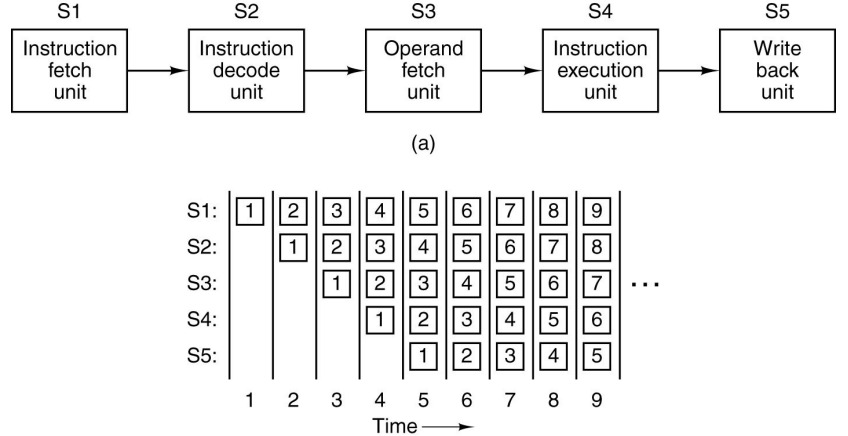
\includegraphics[width=1.00\textwidth]{pipeling}
	\caption{La prima parte della figura mostra una pipeline a 5 stadi. La seconda parte mostra lo stato degli stadi in funzione del tempo}
\end{figure}
Analizziamo questa figura. Durante il primo ciclo di clock lo stadio S1 sta lavorando sull'istruzione 1 prelevandola dalla memoria, durante il ciclo di clock 2 lo stadio S2 sta decodificando l'istruzione 1 mentre lo stadio S1 ha prelevato l'istruzione 2. Durante il ciclo di clock 3 lo stadio S3 preleva gli operandi per l'istruzione 1, lo stadio S2 decodifica l'istruzione 2 e lo stadio S1 preleva l'istruzione 3. Durante il ciclo di clock 4, lo stadio S4 esegue l'istruzione 1, S3 preleva gli operandi per l'istruzione 2, lo stadio S2 decodifica l'istruzione 3 e lo stadio S1 preleva l'istruzione 4. Infine durante il ciclo 5, lo stadio S5 scrive il risultato dell'istruzione 1 e gli altri stadi lavorano sulle prossime istruzioni. \\
Quindi la pipeline può essere paragonato al meccanismo di una catena di montaggio il cui funzionamento è praticamente analogo. \\
Supponiamo che il ciclo di clock della macchina sia di 2 ns e che quindi un'istruzione per percorrere i 5 stadi della pipeline impieghi 10 ns. Quindi, si potrebbe dire che la macchina abbia una velocità di 100 MIPS, ma in realtà le prestazioni sono molto migliori perchè ad ogni ciclo di clock viene completata una nuova istruzione e quindi la velocità reale è di 500 MIPS. \\
L'uso della pipeline permette di bilanciare la \textbf{latenza}, cioè il tempo che un'istruzione impiega per essere elaborata e la \textbf{larghezza di banda del processore}, cioè i MIPS della CPU.
\paragraph{Architettura superscalari} Abbiamo dimostrato che avere una pipeline porta a diversi vantaggi, perciò averne due sarebbe meglio.\\
L'Intel, a partire dal 486, aveva iniziato a dotare i suoi processori di una pipeline e partire dal Pentium di due pipeline a 5 stadi. La pipeline principale chiamata \textbf{pipeline u} che poteva eseguire qualsiasi istruzione Pentium e la \textbf{pipeline v} che poteva eseguire solamente semplici istruzioni su interi. Alcune regole prestabilite determinavano se due istruzioni potevano essere eseguite in parallelo. Se tali istruzioni non erano sufficientemente semplici oppure erano incompatibili la prima veniva eseguita nella pipeline u mentre la seconda veniva trattenuta per essere accoppiata all'istruzione seguente. \\
Segue un'illustrazione di processore a due pipeline:
\begin{figure}[H]
	\centering
	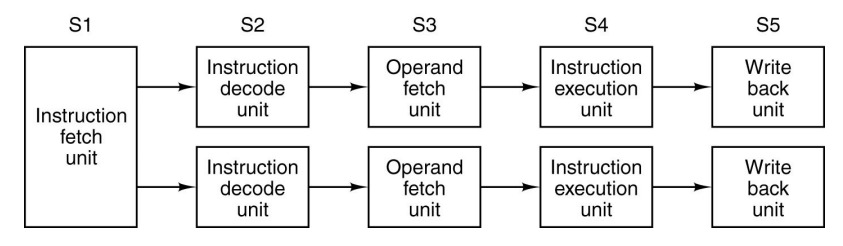
\includegraphics[width=1.00\textwidth]{due_pipeline}
\end{figure}
Analizziamo la figura: in questa situazione una singola unità di fetch preleva due istruzioni alla volta e le inserisce nella pipeline, ognuna delle quali è dotata di una ALU, affinchè le due istruzioni possano essere eseguite in parallelo, non devono esserci conflitti nell'uso delle risorse e nessuna delle due istruzioni deve dipendere dal risultato dell'altra. Come nel caso della singola pipeline o è il compilatore a occuparsi di gestire correttamente questa situazione e quindi se le istruzioni sono incompatibili restituisce un risultato errato oppure i conflitti sono rilevati ed eliminati durante l'esecuzione grazie ad un componente hardware. \\
Anche se si potrebbe pensare un'architettura a quattro pipeline, questo obbligherebbe a duplicare troppi componenti hardware, per questo motivo nelle CPU di alta gamma si utilizza un diverso approccio. \\
Venne coniato il termine di \textbf{architettura superscalare} per indicare questo nuovo tipo di approccio, dove i processori lanciano più istruzioni durante un ciclo di clock e il processore per poter gestire tutte queste istruzioni deve avere più unità funzionali.
Segue un'immagine illustrativa di architettura superscalare:
\begin{figure}[H]
	\centering
	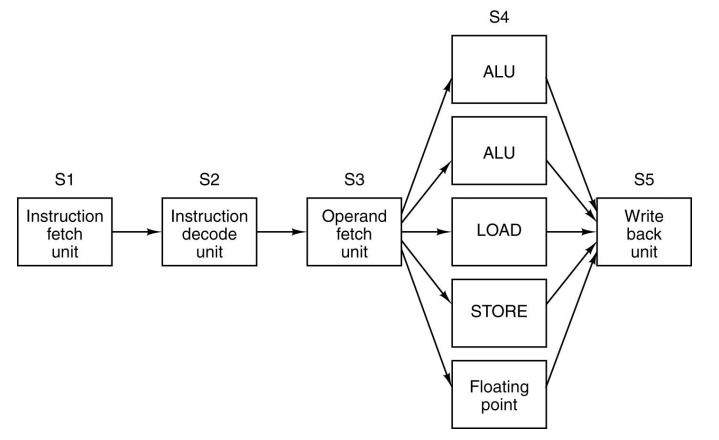
\includegraphics[width=1.00\textwidth]{architettura_superscalare}
\end{figure}
\paragraph{Pipeline: prestazioni} Sia:
\begin{itemize}
	\item \textbf{k}: numero di stadi della pipeline:
	\item \textbf{n}: numero di istruzioni da eseguire:
	\item \textbf{t}: tempo di uno stadio (tempo massimo).
\end{itemize}
Il tempo totale richiesto $T_{pipe}$ per eseguire $n$ istruzioni senza salti è:
\[
T_{pipe} = [k + (n - 1)] \cdot t
\]
Il fattore di velocizzazione della pipeline rispetto ad una architettura tradizionale è:
\[
\dfrac{T_{convezionale}}{T_{pipe}} = \dfrac{nkt}{[k + (n - 1)] \cdot t} = \dfrac{nk}{[k + (n - 1)]}
\]
\paragraph{Pipeline: Trattamento dei salti} Le istruzioni di salto condizionato sono uno dei principali problemi che limitano le istruzioni di una pipeline. \\
Le possibili soluzioni sono:
\begin{itemize}
	\item \textbf{flussi multipli} o multiple stream;
	\item \textbf{prelievo anticipato delle destinazione} o prefetch branch target;
	\item \textbf{buffer circolare} o loop buffer;
	\item \textbf{predizione di salto} o branch prediction;
	\item \textbf{salto ritardato} o delayed branch.
\end{itemize}
\paragraph{Pipeline: Flussi multipli o multiple stream} In questo caso si replicano le parti iniziali della pipeline per consentirle di prelevare entrambe le istruzioni coinvolte nel salto condizionato facendo uso dei due flussi. \\
I problemi di questa soluzione è la generazione dei ritardi per la contesa tra i due flussi e in ciascuno dei due flussi si possono presentare altre istruzioni di salto condizionato.
\paragraph{Pipeline: Prelievo anticipato della destinazione o prefetch branch target} Quando viene riconosciuto un salto condizionato viene anche prelevata anticipatamente la sua destinazione. L'indirizzo è quindi mantenuto fino a quando si dovrà eseguire l'istruzione di salto, in modo che, se occorre compiere il salto, l'indirizzo è già stato prelevato.
\paragraph{Pipeline: Buffer circolare o loop buffer} Si tratta di una piccola e veloce memoria che contiene le ultime $n$ istruzioni prelevate con il fetch. Se occorre effettuare un salto l'hardware controlla se la destinazione si trova nel buffer. In caso affermativo la successiva istruzione viene prelevata dal buffer. \\
I vantaggi di questo approccio è che anticipando il fetch è possibile avere già nella memoria circolare alcune istruzioni evitando di dover far riferimento in memoria alcune volte e nei cicli se le istruzioni dell'intero ciclo riescono a stare nel buffer circolare si ha un massimo vantaggio.
\paragraph{Pipeline: Predizione di salto o branch prediction} 
\begin{itemize}
	\item Previsione di saltare sempre ed è un approccio statico;
	\item Previsione di non saltare mai ed è un approccio statico;
	\item Previsione in base al codice operativo ed è un approccio statico;
	\item Bit taken/not taken ed è un approccio dinamico: ad ogni istruzione di salto condizionato in cache viene associato un bit che memorizza il comportamento recente di quella istruzione e questa informazione viene utilizzata per anticipare il comportamento dell'istruzione di salto;
	\item Tabella della storia dei salti ed è un approccio dinamico: viene usata una tabella con la storia dei salti. Ciascuna riga contiene:
	\begin{itemize}
		\item l'indirizzo dell'istruzione di salto;
		\item un certo numero di bit di storia;
		\item informazioni circa l'istruzione destinazione, solitamente il suo indirizzo.
	\end{itemize}
\end{itemize}
\paragraph{Pipeline: Salto ritardato o delayed branch} Si tratta di ridisporre automaticamente le istruzioni all'interno di un programma in maniera tale che le istruzioni di salto si verifichino in ritardo rispetto al momento in cui effettivamente desiderate.
\subsection{Parallelismo a livello di processore}
In questa forma di parallelismo sono presenti più CPU che lavorano congiuntamente su uno stesso problema. \\
Dato che le CPU continuano a diventare più veloci, prima o poi ci scontrerà con i problemi legati alla velocità della luce. Inoltre, chip più veloci producono anche più calore, e la sua dissipazione costituisce un problema e proprio per questo la velocità delle CPU negli ultimi dieci anni ha subito una stagnazione. \\
Il parallelismo a livello d'istruzione aiuta in parte, ma difficilmente l'uso della pipeline e le operazioni superscalari possono aumentare le prestazioni di un fattore cinque o dieci. Per aumentare le prestazioni di 50, 100 volte maggiori occorre costruire calcolatori con più CPU.
\paragraph{Computer con parallelismo sui dati} Un gran numero di problemi in ambiti computazionali come la fisica, l'ingegneria e la computer graphic vengono trattati con l'utilizzo di cicli e array, o comunque hanno una struttura regolare, infatti spesso gli stessi calcoli vengono eseguiti ripetutamente su diversi insiemi di dati. La loro regolarità li rende adatti a una esecuzione parallela che ne incrementi le prestazioni. Sono stati utilizzati principalmente due metodi per eseguire questi programmi altamente regolari in modo rapido ed efficiente: i processori SIMD e i processori vettoriali. Il primo è visto come un calcolatore parallelo mentre il secondo è considerato come un'estensione di un singolo processore. \\
I computer con parallelismo sui dati, grazie alla loro efficienza, hanno trovato molte applicazioni di successo perchè sono in grado di offrire una grande potenza computazionale con l'utilizzo di un minor numero di transistor rispetto ad altri approcci. \\
Poichè tutti i processori sono in esecuzione sulla stessa istruzione, il sistema ha bisogno di un solo cervello per controllare il computer. Il processore necessita soltanto di uno stadio di prelievo, uno di decodifica e di una logica di controllo. \\
Un processore SIMD consiste di un elevato numero di processori identici che eseguono la stessa sequenza d'istruzioni su insiemi diversi di dati. \\
Le moderne unità di elaborazione grafica, le GPU, si affidano all'elaborazione SIMD per offrire grande potenza di calcolo con pochi transistor. L'elaborazione grafica si presta a processori SIMD perchè la maggior parte degli algoritmi sono altamente regolari, con operazioni ripetute su pixel, vertici, texture e contorni. \\
Agli occhi di un programmatore, i \textbf{processori vettoriali} risultano molto simili a un processore SIMD. Anche questi processori eseguono in modo efficiente una stessa sequenza di operazioni su coppie di dati, anche se tutte le operazioni di addizione sono eseguite da un unico sommatore, altamente strutturato a pipeline. \\
La differenza tra un processore SIMD e un processore vettoriale è che un processore SIMD somma a coppie gli elementi del vettore utilizzando tanti sommatori quanti sono gli elementi dell'array mentre un processore vettoriale utilizza un \textbf{registro vettoriale}.
\paragraph{Multiprocessori} In un processore parallelo sui dati le unità di elaborazione non sono delle CPU indipendenti, dato che c'è un unica unità di controllo condivisa fra tutte. Un sistema \textbf{multiprocessore} è composto da più CPU con una memoria in comune. Dato che ogni CPU può leggere e scrivere una qualsiasi parte della memoria, devono coordinarsi via software per evitare di ostacolarsi a vicenda. Quando due o più CPU riescono a interagire in modo così si dice che sono \textit{tighly coupled}, legate strettamente. \\
Sono possibili vari schemi d'implementazione, il più semplice dei quali consiste nell'avere un singolo bus con più CPU, tutte connesse a un'unica memoria. Ovviamente, se un gran numero di processori veloci tenta di accedere costantemente alla memoria attraverso lo stesso bus si generano dei conflitti. Per evitare questi problemi sono stati sviluppati diversi schemi, uno tra questi è quello di un'architettura in cui ogni processore possiede una propria memoria locale, non accessibile agli altri. Questa memoria è utilizzata per contenere il codice del programma e quei dati che non devono essere condivisi. L'accesso a questa memoria non utilizza il bus principale.
\paragraph{Multicomputer} Se da un lato è relativamente semplice costruire multiprocessori composti da un modesto numero di processori è decisamente più complicato realizzarne di più grandi, perchè è difficile connetterli tutti alla memoria. Per evitare questi problemi, è stata abbandonata l'idea di avere una memoria condivisa e molti progettisti hanno costruito sistemi composti da un gran numero di calcolatori interconnessi, ciascuno dotato di memoria privata. Questi sono detti \textbf{multicomputer}, in questi sistemi le CPU hanno un legame lasco detto \textit{loosely coupled}. \\
Le CPU dei multicomputer comunicano inviandosi messaggi e nel caso di sistemi molto grandi, dato che non è efficiente connettere mutualmente tutti i calcolatori, si utilizzano diverse topologie come griglie 2D e 3D, alberi e anelli e i messaggi tra due calcolatori per spostarsi da sorgente a destinazione devono passare attraverso uno o più macchina intermedie. \\
Visto che è facile programmare i multiprocessori e i multicomputer sono facili da costruire, molte ricerche sono indirizzate alla realizzazione di sistemi ibridi che uniscano le qualità di entrambi. 
\paragraph{Legge di Andahl}  Sia $P$ un processo e supponiamo che sia costituito da una frazione seriale $f_s$ realizzabile in un tempo $T_s$ e da una frazione $f_p$ realizzabile in parallelo in un tempo $T_p$ dove ovviamente $f_s + f_p = 1$ \\
Sia $T_1$ e $T_n$ rispettivamente il tempo di esecuzione del processo su 1 ed $n$ processori:
\[
T_1 = T_s + T_p
\]
$T_1$ può essere normalizzato a 1. \\
\[
T_n = T_s + \dfrac{T_p}{n}
\]
Lo speed-up $S(n)$ con $n$ processori è pari a $\dfrac{T_1}{T_n}$, la \textbf{legge di Andahl}.
\[
S(n) = \dfrac{T_1}{T_n} = \dfrac{1}{f_s + \dfrac{f_p}{n}} = \dfrac{1}{f_s + \dfrac{1 - f_s}{n}} = \dfrac{n}{nf_s + 1 - f_s}
\]
\section{Memoria principale}
La memoria è quella parte del calcolatore dove sono memorizzati programmi e dati. 
\subsection{Locazioni di memoria}
La memoria è costituita da un certo numero di \textbf{celle o locazioni} in ciascuna delle quali si può memorizzare informazioni. \\
Ciascuna cella ha un numero chiamato \textbf{indirizzo} attraverso il quale qualsiasi programma può riferirsi ad essa.
Tutte le celle contengono lo stesso numero di bit, quindi, se una cella contiene $k$ bit potrà assumere al massimo $2^k$ valori.
Attualmente si usa considerare raggruppamenti di bit in \textbf{byte} che sono raggruppati in \textbf{word} che è un'unità di misura della quantità di dati che un processore può elaborare.			
\subsection{Ordinamento dei byte}
All'interno di una parola i byte possono essere numerati da sinistra a destra, la notazione \textbf{big endian}, cioè dal byte più significativo al meno significativo o da destra a sinistra, la notazione \textbf{little endian}, cioè dal byte meno significativo al più significativo.
\begin{figure}[h]
	\centering
	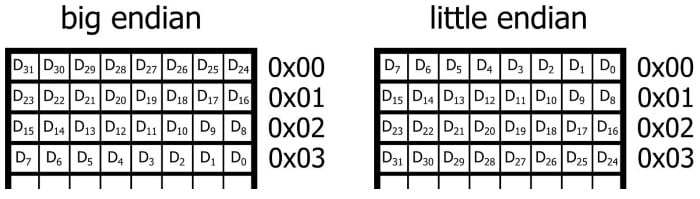
\includegraphics[width=0.70\textwidth]{ordinamento_byte}
\end{figure}\\
\section{Codici correttori di errori}
Occasionalmente le memorie dei calcolatori possono compiere degli errori per via di picchi di tensione sulle linee di alimentazione o per altre cause. \\
Per proteggersi da questi errori, alcune memoria utilizzano dei codici rilevatori e/o correttori di errore. Quando si impiegano questi codici vengono aggiunti dei bit extra a ogni parola della memoria secondo una memoria particolare e grazie ad essi è possibile capire se si sono verificati degli errori.
Supponiamo che una parola di memoria consista di $m$ bit di dati ai quali aggiungiamo $r$ bit di controllo, quindi $n = m + r$ indica la lunghezza totale della parola che verrà chiamata \textbf{parola di codice}.
\subsection{Distanza di Hamming}
Date due parole di codice \textbf{10001001} e \textbf{10110001}, è possibile determinare il numero di bit corrispondenti ai quali differiscono, in questo caso la differenza è di 3 bit.\\
Per determinare il numero di bit diversi, bisogna calcolare lo \textbf{XOR} tra i bit delle due parole e contare quanti bit settati 1 ci sono nel risultato, questo valore viene chiamato \textbf{distanza di Hamming}. Il suo significato principale è che se fra due parole di codice vi è una distanza di Hamming pari a $d$, allora saranno necessari $d$ errori singoli per trasformare una parola nell'altra. \\
Si definisce distanza di Hamming di un codice la minima distanza tra due parole di un codice. \\
\\
Con una parola di memoria a $m$ bit tutte le $2^m$ combinazioni di bit sono legali, ma, per via del modo in cui sono stati calcolati i bit di controllo solo $2^m$ delle $2^n$ parole di codice saranno valide. Se una lettura di memoria restituisce una parole di codice non valida, il calcolatore sa che è avvenuto un errore di memoria.
\\
Le proprietà di rilevazione e di correzione degli errori di una parola di codice dipendono dalla sua distanza di Hamming. Per rilevare $d$ errori è necessaria una parola con distanza $d + 1$, poichè con tale codice non esiste alcun modo in cui $d$ errori singoli possano combinare una parola valida in un'altra parola di codice valida. Per correggere $d$ errori singoli è necessario un codice con distanza $2d + 1$ così le parole di codice legali sono sufficientemente lontana una dall'altra.
Come esempio di codice a correzione di errore consideriamo un codice nel quale si aggiunge un \textbf{bit di parità} scelto in modo che il numero di bit settati a 1 nella parola di codice sia pari (oppure dispari). Un codice di questo tipo ha distanza 2 perchè servono 2 errori singoli per passare da una parola di codice valida a un'altra anch'essa valida. \\
Ciascuna delle $2^m$ parole di memoria legali ha $n$ parole di codice illegali a distanza 1 da essa. Quindi, ciascuna delle $2^m$ parole di memorie legali richiede $n + 1$ stringhe di bit a essa dedicate. Dato che il numero di combinazioni è $2^n$ deve valere la disequazione:
\[
(n + 1)2^m \leq 2^n
\]
che può essere riscritta come:
\[
(m + r + 1) \leq 2^r
\]
Questo limite teorico può essere utilizzato nel \textbf{codice di Hamming}.
\subsection{Codice di Hamming}
\section{Memoria cache}
La memoria cache è localizzata logicamente fra la memoria principale e la CPU, fisicamente ci sono diversi posti possibili dove può essere collocata. \\
La memoria cache è una memoria di piccole dimensioni ma estremamente veloce. Quando la CPU necessita di una parola, la cerca nella cache e solo nel caso non la trova accede alla memoria centrale. \\
L'idea è quella di mantenere nella cache le parole di memoria più utilizzate in modo da ridurre il tempo medio di accesso alla memoria dalla parte della CPU. \\ 
Il buon funzionamento delle memoria cache è dipeso dalla capacità di conservare in essa le informazioni che saranno necessarie. \\
Una delle tecniche più efficaci per migliorare sia la larghezza di banda sia la latenza è l'uso di più cache. Una tecnica elementare che funziona in modo efficace consiste nell'introdurre due cache separate, una per le istruzioni e una per i dati. \\
Il sistema con due cache distinte per i dati e per le istruzioni, chiamato a \textbf{cache separata}, fornisce vari vantaggi. Innanzitutto è possibile far partire le operazioni di memoria indipendentemente per ciascuna cache, raddoppiando la larghezza di banda del sistema. \\
Attualmente molto sistemi di memoria sono ancora più complicati. Spesso tra la memoria centrale e la cache delle istruzioni e dei dati è presente un'altra cache, chiamata \textbf{cache di secondo livello} e in alcuni sistemi, come l'i7, ci possono essere anche 3 o più livelli di cache. \\
Di solito le cache sono annidate , nel senso che l'intero contenuto della cache di primo livello è compreso nella cache di secondo livello e il contenuto di quest'ultima è contenuto in quella di terzo livello. \\
Tutte le cache utilizzano lo stesso modello. La memoria centrale è divisa in blocchi di dimensione fissa chiamati \textbf{linee di cache} che è composta generalmente da 4 a 64 byte consecutivi e linee sono numerate consecutivamente a partire da 0. \\
L'osservazione secondo la quale i riferimenti alla memoria fatti in un breve intervallo temporale tendono a utilizzare solo una piccola parte della memoria totale viene chiamato \textbf{principio di località} che può essere di due tipologie:
\begin{itemize}
	\item \textbf{Principio di località spaziale:} se in un certo istante viene referenziato un indirizzo di memoria è molto probabile che in instanti immediatamente successivi possano venire referenziati indirizzi vicini.
	\item \textbf{Principio di località temporale:} se in un certo istante viene referenziato un indirizzo di memoria è altamente probabile che in istanti immediatamente successivi lo stesso indirizzo possa essere nuovamente referenziato.
\end{itemize}	
Se durante un piccolo intervallo di tempo una parola è letta o scritta \textit{k} volte, il calcolatore dovrà effettuare:
\begin{itemize}
	\item 1 riferimento alla memoria centrale che è più lento $+$ 1 accesso non riuscito alla memoria cache;
	\item $(k-1)$ riferimenti alla cache che sono più veloci.
\end{itemize}
Allora, dati:
\begin{itemize}
	\item \textit{c} = tempo di accesso alla cache;
	\item \textit{m} = tempo di accesso alla memoria.
\end{itemize}
Si ottiene: $t_{memory} = km$ e $t_{cache}=(c+m)+(k-1)c$. \\
Il vantaggio nell'uso della cache è quantificabile in:
\[
\dfrac{t_{cache}}{t_{memory}} = \dfrac{(c+m)+(k-1)c}{km}
\]
Nel caso più generale, definiamo con \textbf{\textit{h}} il numero di richieste che la memoria cache è in grado di soddisfare, questo concetto prende il nome di \textit{hit ratio} ed equivale a: 
\[
\dfrac{number \; of \; hits}{number \; of \; hits \quad + \quad number \; of \; misses} = h \hspace{1cm} 0 \leq h \leq 1
\]
dove il numero di hits, rappresenta il numero di volte che la CPU ha trovato la parola di memoria nella cache, mentre il numero di miss rappresenta quante volte la CPU ha dovuto accedere alla memoria principale. \\
Dopodichè definiamo la \textit{miss ratio}, cioè la frequenza di fallimento, che equivale a: \textbf{\textit{1-h}} e \textbf{\textit{(1 - h)m}} equivale al tempo per far riferimento alla memoria principale e con \textbf{\textit{c}} il tempo per fare riferimento alla cache. \\
Con queste possiamo calcolare il tempo medio di accesso alla cache che equivale a:
\[
Tempo \; medio \; di \; accesso \; = c + (1-h)m
\]
Se $h = 0$ allora il tempo medio di accesso equivale a $c + m$, cioè il tempo per controllare la cache senza trovare nulla e il tempo per accedere alla memoria principale. \\
Se $h = 1$, la miss ratio equivale a 0 e il tempo medio di accesso alla cache equivale proprio al tempo per far riferimento alla cache.		
Esistono due tipologie di cache: 
\begin{itemize}
	\item \textbf{cache a corrispondenza diretta};
	\item \textbf{cache set-associative}.
\end{itemize}
\subsection{Cache a corrispondenza diretta}
Questa è la tipologia di cache più semplice dive ciascun elemento della cache può memorizzare esattamente una linea di cache della memoria centrale. Gli elementi della cache sono composti da 3 campi:
\begin{itemize}
	\item il bit \textit{Valid} che indica se l'elemento è valido oppure no. All'avvio del sistema tutti gli elementi della cache sono marcati come non validi;
	\item il campo \textit{Tag} che è un valore univoco a 16 bit e corrisponde alla linea di memoria dalla quale provengono i dati;
	\item il campo \textit{Data} che contiene una copia del dato della memoria. 
\end{itemize}
In questa tipologia di cache una data parola di memoria può essere memorizzata in un'unica posizione della cache. Per memorizzare e prelevare dati dalla cache, l'indirizzo è diviso in quattro campi:
\begin{itemize}
	\item il campo \textit{Tag} corrisponde ai bit \textit{Tag} dell'elemento della cache;
	\item il campo \textit{Line} indica l'elemento della cache contenente i dati corrispondenti;
	\item il campo \textit{Word} indica a quale parola si fa riferimento all'interno della memoria;
	\item il campo \textit{Byte} non viene utilizzato, ma se si richiede un solo byte esso indica quale byte è richiesto all'interno della parola.
\end{itemize}
Quando la CPU genera un indirizzo di memoria, l'hardware estrae dall'indirizzo il campo LINE e li usa come indice all'interno della cache. Se questo elemento è valido si effettua un confronto fra il campo TAG dell'indirizzo di memoria e il campo TAG dell'elemento della cache, se questi sono uguali l'elemento della cache contiene la parola richiesta e questa situazione è chiamata \textbf{cache hit}. \\
Se l'elemento non è valido oppure se i due campi TAG non corrispondono, il dato richiesto non è presente nella cache e questa situazione è chiamata \textbf{cache miss}.
\subsection{Cache set-associative}
Un problema che si potrebbe riscontrare nelle cache a corrispondenza a diretta è che molte linee di memoria potrebbero essere in competizione per l'utilizzo dello stesso elemento della cache dato che nelle cache a corrispondenza diretta una parola di memoria è memorizzata in un'unica posizione della cache. \\
Una soluzione a questo problema è quello di consentire che in ciascun elemento della cache ci possano essere due o più linee. Una cache con \textit{n} possibili elementi per ciascun indirizzo è chiamata \textbf{cache set-associative a \textit{n} vie}. \\
Queste cache sono più complesse di quelle a corrispondenza diretta, infatti è necessario controllare un insieme di \textit{n} elementi per verificare se la linea richiesta è presente nella cache. \\
L'uso di questa tipologia di cache pone il progettista di fronte a una scelta: quando viene portata all'interno della cache una nuova linea, quale delle presenti deve essere scartata? \\
Un algoritmo che nella maggior parte delle situazioni funziona abbastanza bene è detto \textbf{LRU} che è analogo a quello utilizzato negli algoritmi di sostituzione delle pagine nel modulo di gestione della memoria tramite memoria virtuale. \\ 
Infine, anche le operazioni di scrittura pongono un particolare problema nell'uso della cache. Quando un processore scrive una parola e questa è presente nella cache, deve aggiornare la parola oppure scaricare l'elemento della cache. La soluzione adottata è quella di aggiornare la cache. Ma cosa possiamo dire riguardo l'aggiornamento della copia nella memoria centrale? Ci sono diversi approcci per aggiornare la copia nella memoria centrale. \\ 
Il primo è il \textbf{write-through} che è l'approccio più semplice. Utilizzando questo approccio la copia dell'elemento in memoria centrale viene aggiornato non appena viene modificato l'elemento in cache. Questo metodo è anche il più affidabile, d'altra parte, però, questa tecnica richiede molto traffico verso la memoria, per questo si tende ad utilizzare un altro metodo chiamato \textbf{write-back} o \textbf{write-deferred} cioè \textbf{scrittura ritardata}. Utilizzando questa tecnica, la copia dell'elemento in memoria centrale non viene aggiornato non appena viene modificato l'elemento nella cache, ma viene aggiornato solo quando lo si ritiene opportuno. \\ 
Sempre riguardo le operazioni di scrittura c'è un altro problema: cosa fare se si verifica una scrittura in una locazione di memoria che in quel momento non è memorizzato in cache? Bisogna portare il dato in cache o basta scriverlo in memoria? Nessuna delle due soluzioni è migliore dell'altra ma la maggior parte dei progetti ritardano la scrittura in memoria e portano i dati in cache solo quando si verifica un errore in scrittura: questa tecnica viene chiamata \textbf{write allocation}. \\
Quando si usa una cache a corrispondenza diretta, si tende a non allocare un elemento della cache ad ogni operazione di scrittura perchè andrebbe a complicare un`organizzazione che dovrebbe risultare semplice. 
\subsection{Assemblaggio e tipi di memoria}
Fino ai primi anni '90, le memorie erano prodotto, vendute e installate in un unico chip. \\
Dopo gli anni '90 venne adottata un'organizzazione diversa, vari chip, di 8 o 16 elementi, venivano montati su una scheda a circuiti stampati venduta singolarmente. Questa organizzazione è chiamata \textbf{SIMM} (Single Inline Memory Module) oppure \textbf{DIMM} (Dual Inline Memory Module) a seconda che abbia i connettori allineati su uno o due lati della scheda. Le SIMM sono poco utilizzate adesso e trasferiscono 32 bit per ciclo di clock; le DIMM invece hanno generalmente 120 contatti per lato, rispetto ai soli 72 delle SIMM, e trasferiscono 64 bit per ciclo di clock. Le DIMM più diffuse sono le DDR3, la terza versione delle Double Data Rate. \\
Nei calcolatori portatili si usano delle DIMM di dimensioni inferiori, le \textbf{SODIMM} (Small Outline DIMM). \\
Qui segue un esempio di SIMM e DIMM:
\begin{figure}[H]
	\centering
	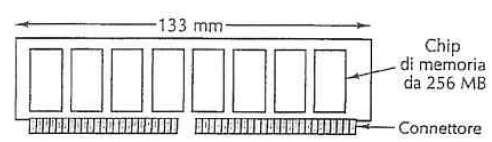
\includegraphics[width=1.00\textwidth]{SIMM_DIMM}
	\caption{Modulo DIMM da 4GB con 8 chip per lato da 256MB}
\end{figure}
\section{Memoria Secondaria}
La memoria centrale non è mai troppo grande, infatti si vorrebbero memorizzare più informazioni rispetto alle reali capacità.
\subsection{Gerarchie di memoria}
La soluzione che viene adottata per memorizzare una grande quantità di dati consiste nell'organizzare gerarchicamente la memoria, come mostrato nella figura: 
\begin{figure}[H]
	\centering
	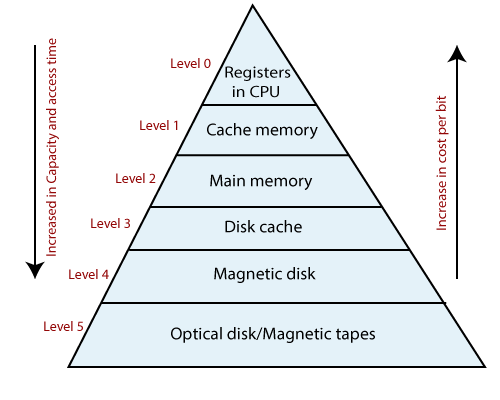
\includegraphics[width=1.00\textwidth]{gerarchia_memoria}
\end{figure}
Muovendosi verso il basso della gerarchia aumentano tre parametri fondamentali:
\begin{enumerate}
	\item il \textbf{tempo di accesso} aumenta man mano che si scende, infatti ai registri delle CPU è possibile accedere in pochi nanosecondi, le cache in tempo che è multiplo di quelle dei registri delle CPU, la memoria centrale è accessibile in una decina di nanosecondi, mentre il tempo di accesso ai dischi è di almeno 10ms e il tempo di accesso per i dischi ottici è sull'ordine dei secondi; 
	\item la \textbf{capacità di memorizzazione} aumenta, infatti i registri possono immagazzinare circa 128 byte, le cache pochi MB; le memoria centrali da decina a migliaia di MB e dischi magnetici possono arrivare anche a decine di GB;
	\item i \textbf{costi unitari} diminuiscono, i costi della memoria centrale è dell'ordine euro/MB, quelli dei dischi magnetici sono 100 volte inferiori e ancora più bassi quelli dei nastri magnetici.
\end{enumerate}
\subsection{Dischi magnetici}
Un disco magnetico consiste di uno o più piatti di alluminio rivestiti di materiale magnetico. \\
La testina del disco, contente un solenoide, sfiora la superficie rimanendo sospesa su un cuscinetto d'aria. Una corrente che passa attraverso la testina magnetizza la superficie che si trova al di sotto, orientando le particelle nella direzione opposte a quella della corrente. Quando la testina passa sopra un'area magnetizzata, viene indotta nella testina una corrente positiva o negativa rendendo possibile la lettura dei bit memorizzati, in questo modo, mentre il piatto ruota, è possibile scrivere e leggere un flusso di bit. \\
La sequenza di bit scritti mentre il disco compie una rotazione completa è chiamata \textbf{traccia}, divisa a sua volta in \textbf{settori} di lunghezza fissa, contenenti un \textbf{preambolo} che permette alla testina di sincronizzasi prima della lettura o della scrittura, il preambolo è seguito dai \textbf{dati} e dopo di essi segue un \textbf{ECC}, un codice per la correzione di errore, come il codice di Hamming o il codice \textbf{Reed-Solomon} che permette la correzione di errori multipli.\\
Tra due settori consecutivi c'è una piccola distanza chiamata \textbf{spazio tra settori}. \\
Alcuni produttori indicano la capacità dei loro dischi nello stato non formattato, come se contenesse solo dati, ma la misura più onesta dovrebbe essere quella formattata che non conta preamboli, ECC e spazi tra dati, la cui capacità è del 15\% inferiore rispetto a quella lorda. \\
\begin{figure}[H]
	\centering
	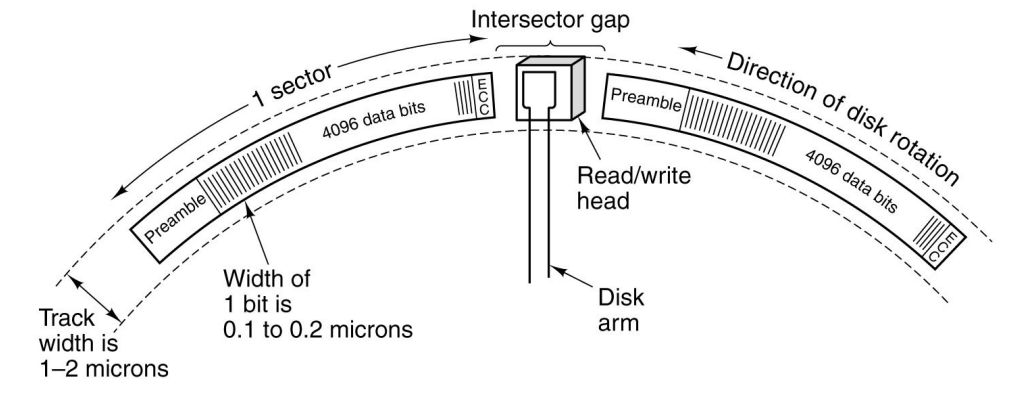
\includegraphics[width=1.00\textwidth]{disco_magnetico}
	\caption{Porzione di una traccia del disco mostrando la composizione dei settori}
\end{figure}
Le tracce, non sono altro che una serie di centri concentrici attorno all'asse di rotazione del disco, la dimensione di ogni traccia dipende da quanto larga è la testina e da quanto accuratamente può essere posizionata. Una traccia non è una scanalatura fisica nella superficie, ma semplicemente una corona circolare di materiale magnetizzato, con piccole aree di sicurezza che la separano da quella più interna a quella più esterna. \\
La densità lineare dei bit lungo le tracce è determinata dalla purezza della superficie e dalla qualità dell'aria, i dischi attuali raggiungono densità tra i 50.000 e 100.000 bit/cm. \\
Al fine di ottenere un'alta qualità della superficie e dell'aria molti dischi sono sigillati durante la fabbricazione per impedire che vi si depositi la polvere, questi dischi sono chiamati \textbf{dischi Winchester}. \\
La maggior parte dei dischi, consiste di più piatti impilati verticalmente in cui ciascuna superficie ha il proprio braccio e la propria testina e l'insieme di tracce alla stessa distanza dal centro è chiamato \textbf{cilindro}. \\
Le prestazioni dei dischi dipendono da diversi fattori:
\begin{itemize}
	\item per leggere o scrivere un settore il braccio deve effettuare la ricerca o \textbf{seek}, cioè lo spostamento radiale sulla posizione corretta, un tempo compreso tra 5ms e 10ms;
	\item una volta che la testina si è posizionata c'è un ritardo, la \textbf{latenza rotazionale} che consiste nell'attesa che il settore desiderato ruoti sotto la testina e visto che i dischi ruotano a 5400, 7200 o 10.800 giri al minuto, il ritardo è tra i 3 e i 6 ms;
	\item il \textbf{tempo di trasferimento} dipende dalla densità lineare e dalla velocità rotazionale che sono tra i 13 e i 16 ms per settore.
\end{itemize}
A causa di preamboli, ECC, spazi tra settori, tempi di ricerca e latenze rotazionali, c'è differenza tra il \textbf{burst rate} e il \textbf{sustained rate} di un disco. \\
Il \textbf{burst rate} è la velocità a cui la testina può leggere i dati dopo essersi posizionata sul primo bit e il calcolatore deve essere in grado di gestire i dati letti a questa velocità, il \textbf{sustained rate}, invece, è la velocità di lettura media nell'arco di un periodo di alcuni secondi, nel quale sono compresi anche i tempi di ricerca e la latenza rotazionale. \\
A ogni disco è associato un \textbf{controllore del disco}, i cui compiti sono accettare i comandi del software, come READ, WRITE e FORMAT, di controllare i movimenti del braccio, di rilevare e correggere gli errori e di convertire i byte letti in uno stream seriale di bit. Alcuni controllori, memorizzano in una cache i settori letti per un loro eventuale riutilizzo.
\subsection{Dischi IDE}
Il sistema operativo leggeva dal disco e scriveva su di esso e successivamente effettuava le chiamate al BIOS, il Basic Input Output System, situato in una memoria di sola lettura. Il BIOS lanciava le istruzioni macchina necessarie per caricare i registri del controllore, che iniziava il trasferimento dei dati. \\
La tecnologia evolse e negli anni '80 si passò alle unità \textbf{IDE}, Integrated Drive Electronics, in cui il controllo era strettamente legato con l'unità, mentre prima si trovava su una scheda separata, mentre le chiamate al BIOS, per questioni di retrocompatibilità, non furono modificate. Secondo questa convezione l'indirizzamento dei settori avveniva specificando i numeri della loro testina, del cilindro e del settore, con la numerazione delle testina che partiva da 0, mentre quella dei settori partiva da 1 forse a causa di un errore del programmatore del BIOS. \\
Utilizzando 4 bit per la testina, 6 bit per il settore e 10 bit per il cilindro, un'unità poteva contenere 16 testine, 63 settori e 1024 cilindri per un totale di 1.032.192 settori che rappresentava una capacità massima di 504MB. \\
Le unità IDE si evolsero nelle unità \textbf{EIDE}, Extended IDE, che avevano uno schema di indirizzamento chiamato \textbf{LBA}, Logical Block Addressing, che numerava i settori da 0 fino a $2^{28} - 1$. Questo schema richiedeva che il controllore convertisse gli indirizzi LBA negli indirizzi della testina, del cilindro e del settore e avevano una capacità massima di 128GB. \\
Lo standard EIDE si evolse, il suo successore fu \textbf{ATA-3}, la versione successiva era \textbf{ATAPI-4} e \textbf{ATAPI-5} con una velocità di trasferimento rispettivamente di 33MB/s e 66MB/s. \\
Con \textbf{ATAPI-6} la dimensione degli LBA fu portato a 48 bit e lo standard \textbf{ATAPI-7} usa l'interfaccia \textbf{serial ATA} per trasferire un bit alla volta su un connettore a 7 pin a una velocità di 150 MB/s e che dovrebbe raggiungere 1.5 GB/s. 
\subsection{Dischi SCSI}
I dischi SCSI, Small Computer System Interface, sono differenti da quelli IDE per quanto riguarda l'organizzazione di cilindri, tracce e settori, ma hanno una diversa interfaccia e una velocità di trasferimento dati molto più elevata. Dei dischi SCSI sono state standardizzate versioni sempre più veloci come mostrato nella figura: 
\begin{figure}[H]
	\centering
	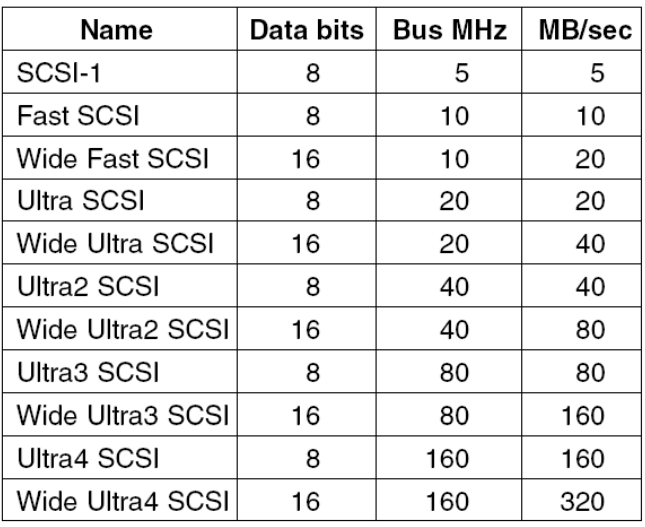
\includegraphics[width=1.00\textwidth]{dischi_SCSI}
\end{figure}
A causa della loro velocità di trasferimento elevata, i dischi SCSI sono lo standard per workstation e server di fascia alta. \\
SCSI non è solo un'interfaccia per hard disk, ma è anche un bus nel quale possono essere collegati un controllore e sette dispositivi, in modo da connettere in serie più dischi SCSI o CD o altre periferiche. Ogni dispositivi SCSI, possiede un ID compreso tra 0 e 7 e due connettori uno per l'input e uno per l'output, dove l'output è connesso con l'input del dispositivo successivo. \\
I controllori SCSI possono funzionare come inziatori o destinatari di comunicazione. Di solito il controllore funziona come iniziatore e lancia comandi ai dischi e ad altre periferiche e indica al destinatario cosa deve fare. I comandi e le risposte avvengono in fase utilizzando vari segnali di controllo per delimitare la fase e arbitrare l'accesso al bus quando più dispositivi tentano di usarlo nello stesso momento e questo è importante perchè consente a tutti i dispositivi SCSI di funzionare contemporaneamente.
\subsection{RAID}
Spesso si utilizza l'elaborazione parallela per velocizzare le prestazioni della CPU. Inoltre, fu anche suggerita l'idea di un'organizzazione a sei dischi per migliorare le prestazioni, l'affidabilità o entrambe. Questa idea fu adottata velocemente e portò a una nuova classe di dispositivi I/O chiamata \textbf{RAID}, Redundant Array of Inexpensive/Independent Disks. \\
L'idea di funzionamento del RAID, consiste nell'installare vicino ad un calcolatore, solitamente un server di grandi dimensioni, un contenitore pieno di dischi, di sostituire il controllore del dischi con un controllore RAID e di continuare le normale operazioni, un RAID quindi dovrebbe apparire come un singolo disco capiente con prestazioni e affidabilità elevate. \\
Tutti i RAID, che appaiono al software come singolo disco, hanno la proprietà di distribuire i dati sulle diverse unità per permetterne la gestione parallela. I RAID hanno dei livelli, solitamente quelli più utilizzati sono quelli che vanno dal livello 0 al livello 5, ogni livello ha un'organizzazione differente con diverse caratteristiche di affidabilità e prestazioni.  
\begin{figure}[H]
	\centering
	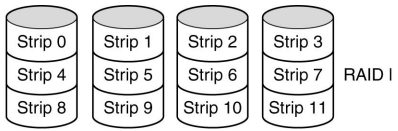
\includegraphics[width=0.75\textwidth]{RAID_0}
	\caption{RAID livello 0}
\end{figure}
Nel RAID di livello 0, il disco virtuale simulato dal RAID è visto che se fosse suddiviso in \textit{strip} consecutive in modo ciclico e questo modo di distribuire le unità è chiamato \textbf{striping}, se ad esempio il software deve leggere un blocco di dati costituito da 4 strip consecutive, il controllore RAID divide questo comando in quattro comandi separati e li farà eseguire in parallelo, in questo modo si ottiene un I/O parallelo senza che il software ne sia a conoscenza. \\
Il RAID di livello 0 lavora meglio quando le richieste sono di grandi dimensioni mentre lavora peggio con i sistemi operativi che richiedono i dati di un settore alla volta, dove il risultato sarà comunque corretto ma le prestazioni sono minori. 
\begin{figure}[H]
	\centering
	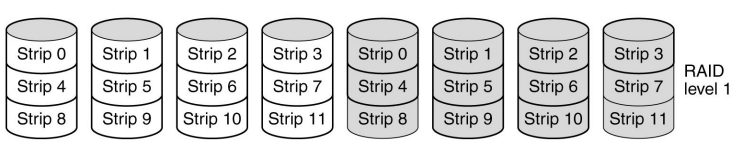
\includegraphics[width=1.00\textwidth]{RAID_1}
	\caption{RAID livello 1}
\end{figure}
Il RAID di livello 1 è un RAID che duplica tutti i dischi, nella foto ad esempio abbiamo 4 dischi primari e 4 di backup. Nel caso di scrittura ogni strip viene scritta due volte, mentre nel caso di lettura è possibile usare entrambe le copie, distribuendo il carico di lavoro su più unità, quindi le operazioni di scrittura non sono migliori, mentre quelle di lettura possono essere fino a due volte migliori. In questo caso il malfunzionamento del disco è facilmente recuperabile grazie ai dischi di backup ma i costi sono molto elevati.
\begin{figure}[H]
	\centering
	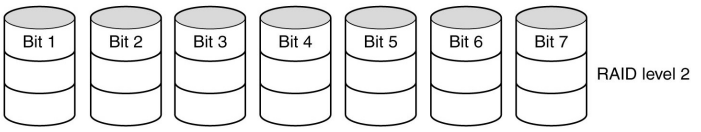
\includegraphics[width=1.00\textwidth]{RAID_2}
	\caption{RAID livello 2}
\end{figure}
Il RAID di livello 2 adotta lo striping dei dati ma questa volta sono di dimensione di mezzo byte, un byte o una parola. \\
Aggiungendo ai 4 bit, cioè al mezzo byte, un codice di Hamming si forma una parola di 7 bit, i cui bit, 1, 2 e 4 sono di parità e i i sette dischi sono sincronizzati per quanto riguarda la posizione die bracci e delle rotazioni. In questo modo è possibile scrivere una parola del codice di Hamming a 7 bit sui sette dischi, usando un bit per ogni disco. Questo permette la lettura/scrittura dei dati in parallelo, d'altra parte, però, è dispendioso ma meno del RAID 1, bisogna gestire la rotazione sincronizzata dei dischi e il controllore ha molto lavoro da svolgere perchè deve verificare rapidamente i bit di controllo.
\begin{figure}[H]
	\centering
	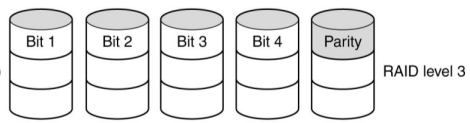
\includegraphics[width=1.00\textwidth]{RAID_3}
	\caption{RAID livello 3}
\end{figure}
Il RAID livello 3, è una versione semplificata del RAID di livello 2. Il bit di parità viene calcolato per ogni parola di dati e poi scritto su un apposito disco. Dato che le parole di dati sono distribuite su più unità, anche in questi caso i dischi devono essere sincronizzati. Si potrebbe pensare che i bit di parità permettono la sola rilevazione degli errori ma non la loro correzione, però, nel caso di rottura di un disco, lo schema permette la correzione degli errori singoli in quanto la posizione del bit errato è conosciuta. Anche in questo caso c'è la lettura/scrittura dei dati in parallelo ma c'è la necessità che la rotazione dei dischi deve essere sincronizzata.
\begin{figure}[H]
	\centering
	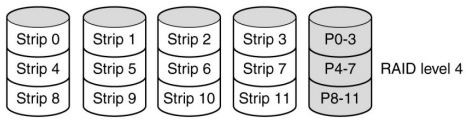
\includegraphics[width=1.00\textwidth]{RAID_4}
	\caption{RAID livello 4}
\end{figure}
Anche il RAID di livello 4 lavorano in base allo strip e non a singole parole con parità e non richiedono la sincronizzazione dei dischi. Il RAID di livello 4 è come il RAID di livello 0, con una parità strip-per-strip scritta su un disco aggiuntivo e se un disco si guasta è possibile ricalcolare i byte persi grazie al disco di parità. Il RAID di livello 4 protegge dalla perdita di un disco, ma ha prestazioni scarse quando si aggiornano piccole quantità di dati, perchè se si modifica un settore, è necessario leggere tutti i dischi perchè bisogna ricalcolare e riscrivere la parità. Inoltre, il disco di parità rallenta il sistema, a causa del grande carico di lavoro che pesa su di esso.
\begin{figure}[H]
	\centering
	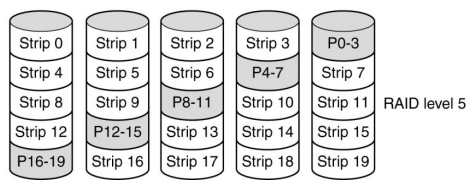
\includegraphics[width=1.00\textwidth]{RAID_5}
	\caption{RAID livello 5}
\end{figure}
Il RAID di livello 5 elimina il disco di parità in quanto distribuisce uniformemente i bit di parità su tutti i dischi, in modalità \textit{round robin}, però quando si verifica un guasto la ricostruzione del suo contenuto è un processo complesso.
\subsection{Dischi a stato solido}
I dischi basati su memoria flash non volatile, gli SSD, si stanno diffondendo grazie all'alta velocità. Un guasto di cui può soffrire un transistor è dovuto all'iniezione a caldo, che è un'avaria per cui una carica di elettroni viene rinchiusa all'interno del transistor, lasciandolo in uno stato di blocco, accesso o spento. Quest'avaria è stata sfruttata per creare una nuova memoria non volatile. \\
I CD-R permettono ai privati e alle società di copiare facilmente i CD-ROM spesso in violazione dei diritti d'autore e sono stati ideati vari schemi per ostacolare questa pirateria e far sì che sia difficile leggere un CD-ROM se non utilizzando il software fornito dall'autore stesso.
\subsection{CD-Riscrivibili}
Anche se abitualmente vengono usati supporti che permettono un'unica struttura, c'è una grande richiesta di CD-ROM riscrivibili. \\
Una tecnologia disponibile è quella dei \textbf{CD-RW}, Rewritable, che impiegano una lega di argento, indio, antimonio e tellurio per registrare i dati. Questa lega ha due stati stabili, quello cristallino e quello amorfo, che hanno proprietà riflettenti diverse. \\
I lettori CD-RW utilizzano laser che funzionano a tre potenze distinte. Alla potenza più elevata il laser scioglie la lega portandola dallo stato cristallino altamente riflettente a quello amorfo che ha una riflettività minore e che rappresenta un \textit{pit}. Allo stato medio la lega si scioglie e si ricompone nello stato cristallino per tornare a rappresentare un \textit{land}.\\
I CD-R non sono stati sostituiti completamente anche perchè il fatto che un CD-R non possa essere cancellato rappresenta un vantaggio per backup dei dischi.
\subsection{DVD}
Negli anni '90, con il miglioramento della tecnologie, sono stati sviluppati dischi ottici più economici e con capacità maggiore. Inoltre, in questo periodo, Hollywood stava cercando un modo per sostituire le videocassette analogiche con dei dischi ottici in modo da offrire una qualità maggiore e più economici in termini di costi e di spazio occupato. \\
Perciò, furono ideati ai DVD, Digital Video Disk ma che ora significa Digital Versatile Disk. I DVD sono progettati in modo molto simile ai CD, le novità riguardano l'uso di pit più piccoli, una spirale più stretta e un laser rosso. \\
Questi miglioramenti permettono una capacità che arriva fino a 4,7 GB e una velocità di 1,4 MB/S. Utilizzando la compressione MPEG-2 un disco DVD può memorizzare 133 minuti di video a schermo intero, con otto versioni di colonne sonore e sottotitoli in 32 lingue diverse. \\
Tuttavia, per memorizzare maggiori informazioni sono stati definiti quattro formati: 
\begin{enumerate}
	\item singolo lato, singolo strato, 4,7GB;
	\item singolo lato, doppio strato, 8,5 GB;
	\item doppio lato, singolo strato, 9,4 GB;
	\item doppio lato, doppio strato, 17 GB.
\end{enumerate}
Esistono queste versioni a causa di politica perchè Philips e Sony volevano dischi a singolo lato e doppio strato, mentre Toshiba e Time Warner volevano dischi a doppio lato e doppio strato ma Philips e Sony credevano che la gente non fosse disposta a girare i dischi e infatti avevano ragione. \\
La tecnologia a doppio strato ha uno stato riflettente nella parte bassa, coperto da uno semiriflettente. A seconda del punto in cui il laser è messo a fuoco, questo rimbalza su un livello oppure sull'altro, il livello più basso richiede che \textit{pit} e \textit{land} siano leggermente più grandi per essere leggibili in modo affidabile, infatti la sua capacità è inferiore rispetto allo strato superiore. \\ 
I dischi a doppio lato sono creati prendendo due dischi a singolo lato e incollandoli uno contro l'altro. \\
I DVD sono stati pensati principalmente per film, infatti tra le funzionalità troviamo l'omissione in tempo reale di scene scabrose, l'audio a sei canali e il supporto per \textit{Pan-and-Scan} che permette di decidere come tagliare le bande laterali dei film. Un altro aspetto è la scelta intenzionale di rendere incompatibili i dischi previsti per gli Stati Uniti rispetto a quelli previsti per l'Europa e altri continenti, in quanto i nuovi film escono sempre prima negli Stati Uniti.
\subsection{Blu-Ray}
I Blu-Ray sono un'evoluzione dei DVD e potrebbero diventare obsoleti a causa di essi, infatti i Blu-Ray utilizzano il laser blu a differenza di quello rosso. Il laser blu hanno una lunghezza d'onda più piccola, il che permette una messa a fuoco più accurata e l'uso di \textit{pit} e \textit{land} più piccoli, infatti i Blu-Ray a singolo strato hanno una capacità di 25 GB e quelli a doppio lato di 50 GB e la velocità di trasferimento è di 4,5 MB/s.
\chapter{Algebra di Boole e i circuiti logici}
		\section{Porte logiche}
			La base hardware di tutti i calcolatori digitali è costituita da delle \textbf{porte logiche}, che sono dei piccolo dispositivi digitali, ciascuno dei quali calcola una diversa funzione di questi segnali. \\
			Le porte logiche più semplici sono NOT, AND, OR e sono i principali elementi costitutivi del livello logico digitale e con le coppie, \textbf{(NOT, AND)} e \textbf{(NOT, OR)}  è possibile costruire qualsiasi altra porta logica. \\
			Il funzionamento delle singole porte logiche rientrano nel campo dei \textbf{livello dei dispositivi} che si trova al di sotto del livello logico digitale.	
		\section{Logica proposizionale: le proposizioni}
			Le frasi affermative hanno una caratteristica che le differenzia dalle altre: possono essere \textbf{vere} o \textbf{false}.
			Nella logica proposizionale queste sono chiamate \textbf{proposizioni}.
			Una proposizione si chiama \textbf{elementare} o \textbf{semplice} se contiene solo un predicato.
			Una proposizione \textbf{composta} è costituita da diverse proposizioni elementari unite da avverbi e/o congiunzioni, da simboli come \textbf{NOT, OR} e \textbf{AND}.
			L'algebra di Boole è costituita da variabili, costanti, operatori e proprietà.
			La variabile booleana è un'entità che può assumere due valori, 0 o 1. \\
			Una funzione booleana ha una o più variabili di input e genera un valore di output che dipende soltanto dai valori di queste variabili. \\
			Una funzione booleana può essere descritta mediante una tabella di $2^n$ righe dato che esistono $2^n$ possibili combinazioni di input e ogni riga indica il valore della funzione per una data combinazione degli input, questa tabella prende il nome di \textbf{tabella di verità}. \\
			La \textbf{tabella di verità} non è l'unico modo per descrivere una funzione booleana, anzi, diventa un metodo inefficiente nel momento in cui il numero di variabili di input diventa elevato. \\
			Una funzione booleana, può essere descritta come una somma di prodotti, ad esempio: 
			\[
			f: ABC + \overline{A}BC + \overline{ABC}
			\]
			Sulle variabili booleane si possono eseguire le seguenti operazioni booleane elementari:
			\begin{itemize}
				\item \textbf{NOT}
				\item \textbf{OR}
				\item \textbf{AND}
				\item \textbf{XOR}
				\item \textbf{NOR}
				\item \textbf{NAND}
			\end{itemize}
			\subsection{Operatore NOT}
			L'operatore NOT restituisce il valore inverso a quello in entrata, in altre parole se in ingresso riceve la variabile booleana A restituisce il suo valore complementato.
			\\
			\\
			
			\begin{tabular} {c|c}
				\textbf{A} & $\mathbf{\overline{A}}$ \\
				\hline
				0 & 1 \\
				1 & 0
			\end{tabular}
			\begin{figure}[h]
				\centering
				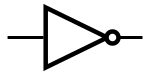
\includegraphics[width=0.15\textwidth]{NOT}
				\caption{Circuito logico NOT}
			\end{figure}
			\subsection{Operatore OR - Somma logica}
			L'operatore OR, detta anche somma logica, restituisce come valore 1 se almeno uno degli elementi è 1, mentre restituisce 0 se sono tutti 0. L'operatore OR deve prendere in ingresso 2 o più variabili booleane.
			\\
			Tabella di verità con due variabili boolenae:
			\\
			\\
			\begin{tabular}{c|c|c}
				\textbf{A} & \textbf{B} & $\mathbf{A + B}$ \\
				\hline
				0 & 0 & 0 \\
				0 & 1 & 1 \\
				1 & 0 & 1 \\
				1 & 1 & 1 \\
			\end{tabular}
			\begin{figure}[h]
				\centering
				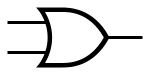
\includegraphics[width=0.15\textwidth]{OR}
				\caption{Circuito logico OR}
			\end{figure}
			\subsection{Operatore AND - Prodotto logico}
			L'operazione AND, detta anche prodotto logico, restituisce come valore 1 se e solo se tutti gli altri elementi hanno valore 1, in caso contrario restituisce 0. L'operatore AND deve prendere in ingresso 2 o più variabili booleane.
			\\
			Tabella di verità con due variabili booleane:
			\\
			\\
			\begin{tabular}{c|c|c}
				\textbf{A} & \textbf{B} & $\mathbf{A * B}$ \\
				\hline
				0 & 0 & 0 \\
				0 & 1 & 0 \\
				1 & 0 & 0 \\
				1 & 1 & 1 \\
			\end{tabular}
			\begin{figure}[h]
				\centering
				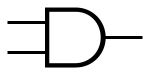
\includegraphics[width=0.15\textwidth]{AND}
				\caption{Circuito logico AND}
			\end{figure}
			\subsection{Operatore XOR - Somma modulo 2}
			L'operatore XOR, detto anche \textbf{OR Esclusivo} o \textbf{somma modulo 2}, restituisce come valore 1 se e solo se il numero degli operandi con valore 1 è \textbf{dispari}, mentre restituisce 0 in tutti gli altri i casi.
			\\
			Tabella di verità con due variabili booleane: 
			\\
			\\
			\begin{tabular}{c|c|c}
				\textbf{A} & \textbf{B} & $\mathbf{A \oplus B}$ \\
				\hline
				0 & 0 & 0 \\
				0 & 1 & 1 \\
				1 & 0 & 1 \\
				1 & 1 & 0 \\
			\end{tabular}
			\begin{figure}[h]
				\centering
				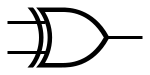
\includegraphics[width=0.15\textwidth]{XOR}
				\caption{Circuito logico XOR}
			\end{figure} \\
			Lo XOR possiamo ricavarlo usando le leggi di De Morgan: \\
			$A \oplus B = \overline{A}B + A\overline{B}$
			\subsection{Operatore NOR}
			Rappresenta l'OR negato $C = NOR(A, B) = \overline {A + B}$.
			\\
			Tabella di verità con due variabili booleane:
			\\
			\\
			\begin{tabular}{c|c|c|c}
				\textbf{A} & \textbf{B} & $\mathbf{A + B}$ & $\mathbf{\overline{A + B}}$ \\
				\hline
				0 & 0 & 0 & 1\\
				0 & 1 & 1 & 0\\
				1 & 0 & 1 & 0\\
				1 & 1 & 1 & 0\\
			\end{tabular}
			\begin{figure}[h]
				\centering
				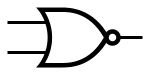
\includegraphics[width=0.15\textwidth]{NOR}
				\caption{Circuito logico NOR}
			\end{figure}
			\subsection{Operatore NAND}
			Rappresenta l'AND negato $C = NAND(A, B) = \overline{A * B}$.
			\\
			Tabella di verità con due variabili booleane:
			\\
			\\
			\begin{tabular}{c|c|c|c}
				\textbf{A} & \textbf{B} & $\mathbf{A * B}$ & $\mathbf{\overline{A * B}}$ \\
				\hline
				0 & 0 & 0 & 1\\
				0 & 1 & 0 & 1\\
				1 & 0 & 0 & 1\\
				1 & 1 & 1 & 0\\
			\end{tabular}
			\begin{figure}[h]
				\centering
				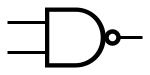
\includegraphics[width=0.15\textwidth]{NAND}
				\caption{Circuito logico NAND}
			\end{figure}
			\subsection{Identità e proprietà dell'algebra booleana}
			Spesso i progettisti cercano di ridurre il numero di porte logiche utilizzate nei loro prodotti per limitare le dimensioni delle schede con i circuiti stampati, diminuire il consumo energetico e aumentare la velocità. Per fare ciò il progettista deve trovare un altro circuito che calcoli la stessa funzione di quello originario, ma che sia composto di un numero inferiore di porte, per verificare poi che i due circuiti siano equivalenti basta controllare se le rispettive tabelle di verità siano uguali. \\
			Per fare ciò, spesso è possibile fattorizzare l'espressione, come avviene nell'algebra ordinaria, ma bisogna conoscere alcune \textbf{identità fondamentali:}
			\begin{table}[H]
				\centering
				\begin{tabular}{|l|c|c|}
					\hline
					\textbf{Nome} & \textbf{Forma AND} & \textbf{Forma OR} \\
					\hline
					Elemento neutro & $1 \cdot A = A$ & $0 + A = A$ \\
					\hline
					Assorbimento & $0 \cdot A = 0$ & $1 + A = 1$ \\
					\hline
					Idempotenza & $A \cdot A = A$ & $A + A = A$ \\
					\hline
					Complementazione & $A \cdot \overline{A} = 0$ & $A + \overline{A} = 1$ \\
					\hline
					Proprietà commutativa & $AB = BA$ & $A + B = B + A$ \\
					\hline
					Proprietà associativa & $(AB)C = A(BC)$ & $(A + B) + C = A + (B + C)$ \\
					\hline
					Proprietà distributiva & $A + BC = (A + B)(A + C)$ & $A(B + C) = AB + AC$ \\
					\hline
					Legge di assorbimento & $A(A + B) = A$ & $A + AB = A$ \\
					\hline
					2° legge di assorbimento & $A(A + B) = AB$ & $A + \overline{A}B = A + B$ \\
					\hline
					Legge di De Morgan & $\overline{AB} = \overline{A} + \overline{B}$ & $\overline{A + B} = \overline{A} \cdot \overline{B}$ \\
					\hline
				\end{tabular}
				\caption{Proprietà dell'algebra booleana}
				\label{tab:boolean_algebra}
			\end{table}
			\begin{proof}{Dimostrazione prima legge di Demorgan: \[
					\overline{A * B} = \overline{A} + \overline{B}
					\]} 
			\begin{center}
			\begin{tabular}{c|c|c|c|c|c|c}
				$\mathbf{A}$ & $\mathbf{B}$ & $\mathbf{A * B}$ & $\mathbf{\overline{A * B}}$ & $\mathbf{\overline{A}}$ & $\mathbf{\overline{B}}$ & $\mathbf{\overline{A} + \overline{B}}$ \\
				0 & 0 & 0 & \color{red}\textbf{1} & 1 & 1 & \color{red}\textbf{1}\\
				0 & 1 & 0 & \color{red}\textbf{1} & 1 & 0 & \color{red}\textbf{1}\\
				1 & 0 & 0 & \color{red}\textbf{1} & 0 & 1 & \color{red}\textbf{1}\\
				1 & 1 & 1 & \color{red}\textbf{0} & 0 & 0 & \color{red}\textbf{0}\\
			\end{tabular}
			\end{center}
			\end{proof}
			\begin{proof}{Dimostrazione seconda legge di Demorgan: \[
					\overline{A + B} = \overline{A} * \overline{B}
					\]}
				\begin{center}
					\begin{tabular}{c|c|c|c|c|c|c}
						$\mathbf{A}$ & $\mathbf{B}$ & $\mathbf{A + B}$ & $\mathbf{\overline{A + B}}$ & $\mathbf{\overline{A}}$ & $\mathbf{\overline{B}}$ & $\mathbf{\overline{A} * \overline{B}}$ \\
						0 & 0 & 0 & \color{red}\textbf{1} & 1 & 1 & \color{red}\textbf{1}\\
						0 & 1 & 1 & \color{red}\textbf{0} & 1 & 0 & \color{red}\textbf{0}\\
						1 & 0 & 1 & \color{red}\textbf{0} & 0 & 1 & \color{red}\textbf{0}\\
						1 & 1 & 1 & \color{red}\textbf{0} & 0 & 0 & \color{red}\textbf{0}\\
					\end{tabular}
				\end{center}
			\end{proof}
			\section{Circuiti logici digitali elementari}
			Ai giorni d'oggi sono pochi i circuiti costruiti porta per porta in quanto i componenti elementari sono rappresentati da moduli contenenti un certo numero di porte.
			\subsection{Circuiti integrati}
			Le porte logiche vengono vendute in unità chiamate \textbf{circuiti integrati} o \textbf{chip} e non è altro che un pezzo rettangolare di silicio la cui grandezza dipende dal numero di porte necessarie per implementare i componenti del chip. Questi chip sono montati in supporti di plastica che possono essere anche più grandi dei circuiti ospitati nel caso in cui siano necessari molti pin contatti per collegare il chip al mondo esterno. Solitamente i chip più piccoli, come la RAM, utilizzano un supporto di tipo \textbf{DIP} cioè a due file di pin, mentre i circuiti più grandi utilizzano un supporto di tipo \textbf{PGA} con dei pin simili a quelli di supporti di tipo DIP, o utilizzano un supporto di tipo \textbf{LGA}, che hanno invece piccoli pad piatti sul fondo del chip che si inserisce applicando una forza rivolta verso il basso, la CPU ne è un esempio. 
			\section{Reti combinatorie}
			Molte applicazioni della logica digitale richiedono un circuito, chiamato \textbf{rete combinatoria} con più input e più output, dove gli output sono determinati dalle varie combinazioni degli input, ed esistono anche circuiti che generano un valore di output che non dipendono solo dalle variabili d'ingresso ma anche dei valori memorizzati nel caso in cui un circuito contiene elementi di memoria, come il Latch.
			\subsection{Multiplexer}
			Il multiplexer si occupa di dirigere $2^n$ segnali di ingresso in un singolo segnale di uscita secondo $n$ linee di controllo. Queste input di controllo permettono di selezionare un segnale di ingresso che viene "instradato" verso l'esterno. \\ 
			Una possibile applicazione di questo circuito è la conversione dei dati da parallelo a seriale, infatti se si immettono 8 bit di dati nelle linee di input e si fa variare il valore delle linee di controllo da 000 a 111, si ottengono sulla linea degli output gli 8 bit in serie, la conversione da parallelo a seriale lo si riscontra nelle tastiere: quando si prema un tasto viene generato un numero a 7 o 8 bit che deve essere inviato su un collegamento seriale come la USB. 
			\\
			\begin{figure}[H]
				\centering
				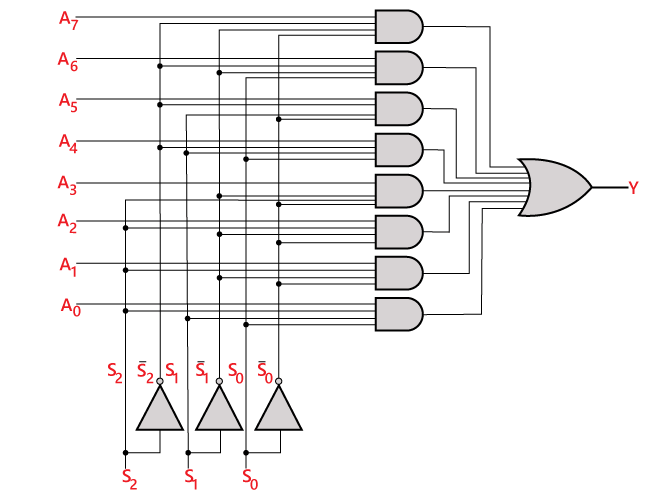
\includegraphics[width=1.00\textwidth]{multiplexer}
				\caption{Circuito logico del multiplexer}
			\end{figure} 
			Le tre linee di controllo $S_0, S_1, S_2$ della figura generano un numero a 3 bit che specifica quale delle 8 otto linee di input deve essere instradato verso l'OR e quindi verso l'uscita. Tra le 8 otto linee di input, 7 di queste, indipendentemente dal valore generato dalle 3 linee di controllo generano sempre valore 0, mentre quella rimanente produrrà o 0 o 1, a seconda del valore della linee di ingresso selezionata.
			\subsection{Decodificatore}
			Il decodificatore accetta come input $n$ segnali di ingresso, che generano un numero a $n$ bit che sarà poi utilizzato dal decodificatore per impostare una sola dei $2^n$ segnali di uscita. \\
			Per capire in quali situazioni può essere utile questo circuito, si può immaginare una memoria di otto chip, da 256 MB ciascuno. Quando si fornisce alla memoria un indirizzo, si utilizzano i suoi 3 bit più significativi per selezionare uno degli otto chip.
			\begin{figure}[H]
				\centering
				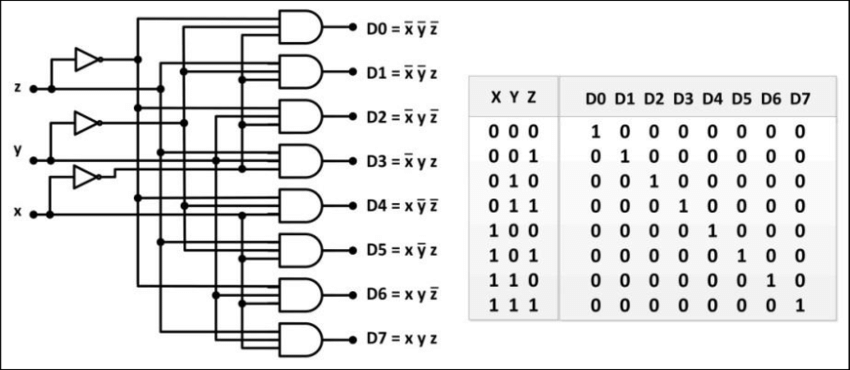
\includegraphics[width=1.00\textwidth]{Decodificatore}
				\caption{Circuito logico e tabella di verità del decodificatore}
			\end{figure} 
			\subsection{Comparatori}
			Il comparatore permette di confrontare due stringhe di bit. Il circuito è basato sulla porta logica XOR che può produrre i seguenti valori:
			\begin{itemize}
				\item 0 se gli input sono uguali;
				\item 1 se se gli input sono diversi;
			\end{itemize}
			Quindi, se tutti gli input di ingresso sono uguali, tutte le porte XOR dovranno generare valore 0, tutti questi valori possono poi essere connessi a una porta OR in modo che restituisca 0 quando gli input sono uguali e 1 quando sono diversi. Se vogliamo avere il risultato contrario, quindi 1 quando gli input sono uguali e 0 quando sono diversi, possiamo utilizzare la porta NOR.\\
			\begin{figure}[H]
				\centering
				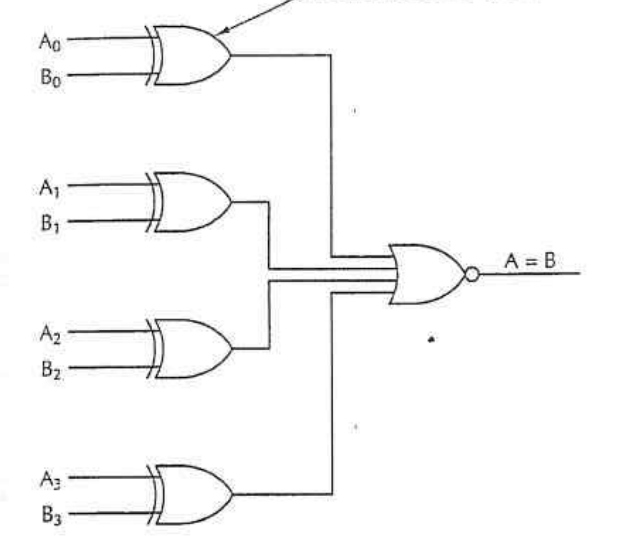
\includegraphics[width=0.60\textwidth]{Comparatore}
				\caption{Esempio di comparatore a 4 bit}
			\end{figure}
			\subsection{Array logici programmabili}
			Un chip molto generale che permette di calcolare somme di prodotti è l'\textbf{array logico programmabile} o \textbf{PLA}. \\
			Questo chip ha 12 ingressi e al suo interno questi valori vengono invertiti quindi il numero totale di ingressi diventa 24. Il cuore del circuito è costituito da una schiera di 50 porte AND che possono avere come input qualsiasi sottoinsieme dei 24 segnali di input. Una matrice di $24\times50$ bit fornita dall'utente determina le connessioni desiderate tra i segnali di input e le 50 porte AND. L'uscita del circuito consiste in 6 porte OR che possono avere anche fino a 50 input. Anche in questo caso l'utente deve fornire una matrice $50\times6$ per specificare quali connessioni instaurare. Il chip ha 20 pin in tutto, 12 per gli ingressi, 6 per le uscite e 2 per la tensione e la messa a terra.
			\begin{figure}[H]
				\centering
				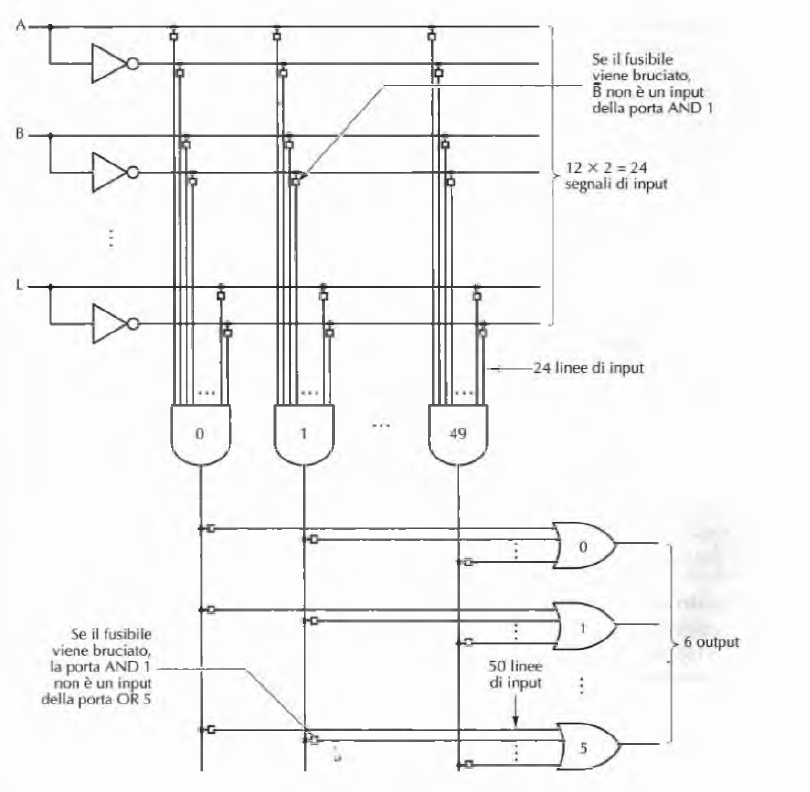
\includegraphics[width=1.00\textwidth]{PLA}
				\caption{Esempio di PLA a 12 ingressi e 6 uscite}
			\end{figure}
			\section{Circuiti per l'aritmetica}
			\subsection{Registri a scorrimento}
			I registri a scorrimento sono costituiti da una catena di celle di memoria a 1 bit interconnesse fra loro e ad ogni impulso di clock essi consentono lo scorrimento da una cella a quella immediatamente adiacente. 
			\begin{figure}[H]
				\centering
				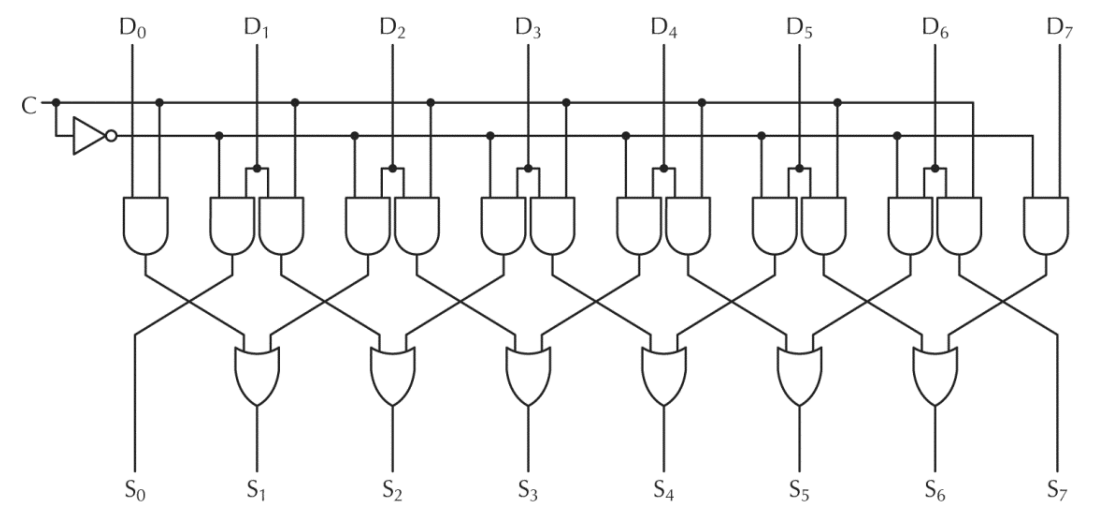
\includegraphics[width=1.00\textwidth]{registri_scorrimento}
				\caption{Registro a scorrimento con 8 input e 8 output}
			\end{figure}
			Il circuito in figura, presenta 8 input e 8 output. Gli input sono collegati alle linee 
			$D$, mentre l'output, che corrisponde all'input traslato di un bit, è disponibile sulle linee $S$. La linea di controllo $C$ ha valore 0 se lo spostamento deve avvenire verso sinistra e 1 il contrario. \\
			Nel caso di uno spostamento a sinistra viene inserito uno 0 nel bit 7 e nel caso di spostamento a destra viene inserito uno 0 nel bit 0. \\
			Nel circuito, per tutti i bit che non sono all'estremità c'è una coppia di porte AND, quando $C = 1$ la porta che si trova a destra viene abilitata e dato che questa porta è collegata all'input della porta OR alla sua destra, si ottiene uno scorrimento verso destra. Se $C = 0$ accade il contrario, cioè viene attivata la porta AND a sinistra.
			\subsection{Unità di semi somma}
			L'unità di semi somma esegue la somma di due bit $A$ e $B$ e la presenta sull'uscita $S$; della somma ne viene calcolato anche il riporto $C$ o $R$ senza tener conto di un riporto precedente.
			\\
			\textbf{Tabella di verità half adder: }
			\\
			\\
			\begin{tabular}{c|c|c|c}
				\textbf{A} & \textbf{B} & \textbf{S} & $\mathbf{C_o}$ \\
				\hline
				0 & 0 & 0 & 0 \\
				0 & 1 & 1 & 0 \\
				1 & 0 & 1 & 0 \\
				1 & 1 & 0 & 1 \\
			\end{tabular}
			\begin{figure}[H]
			\centering
			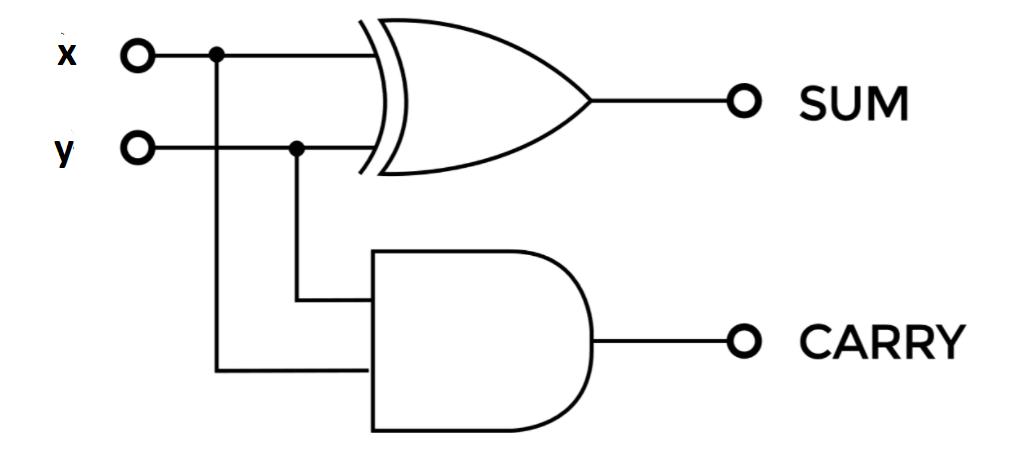
\includegraphics[width=0.75\textwidth]{HALF_ADDER}
			\caption{Circuito logico Half adder}
			\end{figure}
			\subsection{Full adder}
			Il full adder o sommatore completo è un circuito logico con tre ingressi e due uscite.
			Questo circuito, è capace di sommare due bit tenendo conto di un eventuale riporto precedente.\\ 
			\textbf{Tabella di verità full adder: } \\ \\
			\begin{tabular}{c|c|c|c|c}
				\textbf{A} & \textbf{B} & $\mathbf{C_{in}}$ & \textbf{S} & $\mathbf{C_o}$ \\
				\hline
				0 & 0 & 0 & 0 & 0 \\
				0 & 0 & 1 & 1 & 0 \\
				0 & 1 & 0 & 1 & 0 \\
				0 & 1 & 1 & 0 & 1 \\
				1 & 0 & 0 & 1 & 0 \\
				1 & 0 & 1 & 0 & 1 \\
				1 & 1 & 0 & 0 & 1 \\
				1 & 1 & 1 & 1 & 1 \\
			\end{tabular}
			\begin{figure}[H]
				\centering
				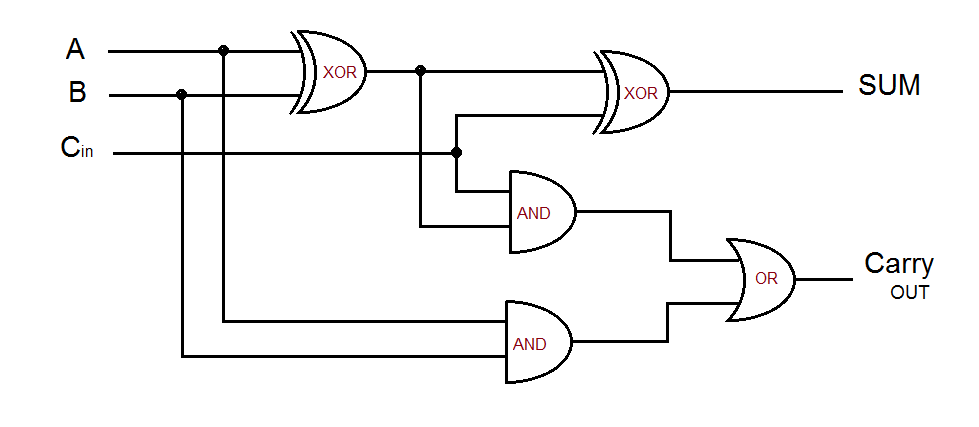
\includegraphics[width=1.00\textwidth]{full_adder}
				\caption{Circuito logico del full adder}
			\end{figure}
			Dalla figura notiamo che la somma vale 1 se una o tre delle tre linee di ingresso valgono 1, altrimenti valgono 0, quindi si può comporre facendo lo XOR fra $A$ e $B$ e successivamente lo XOR con $C_{in}$. \\
			Per quanto riguarda il riporto, invece, il riporto c'è se $A$ e $B$ valgono 1 oppure se uno dei due vale 1 e $C_{in}$ vale 1, cioè se lo XOR fra $A$ e $B$ vale 1 e se $C_{in}$ vale 1.\\
			Il full adder quindi è composto da due half adder.
			\section{Unità aritmetico logica}
			La maggior parte dei calcolatori contiene un unico circuito in grado di effettuare le operazioni AND, OR e somma di due parole. Di solito un circuito di questo tipo funzionante su parole a $n$ bit è costituito a partire da $n$ circuiti identici per le singole posizione dei bit.
			\begin{figure}[H]
				\centering
				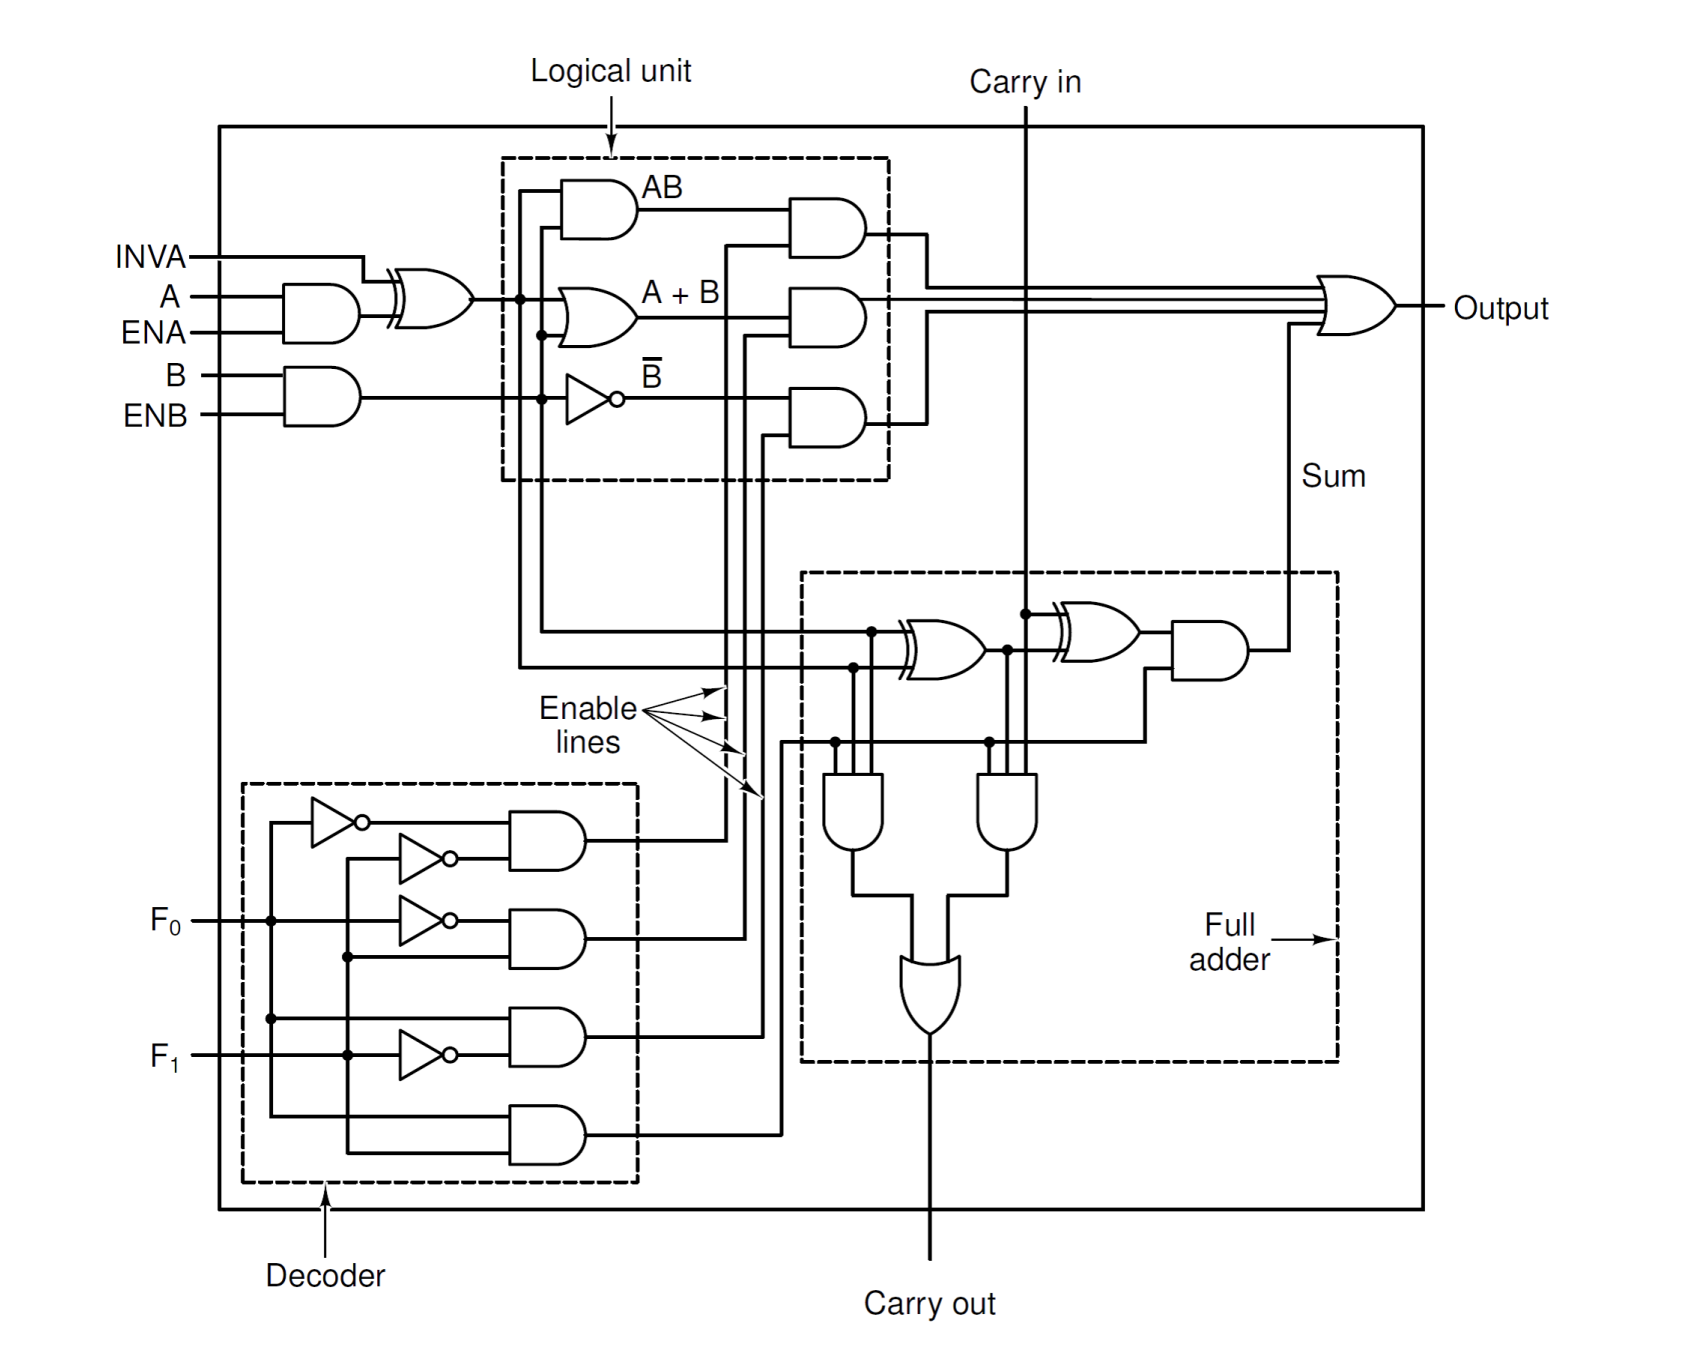
\includegraphics[width=1.00\textwidth]{ALU_1bit}
				\caption{ALU a 1 bit}
			\end{figure}
			Nella figura, in basso a sinistra, troviamo un decodificatore a 2 bit che permette di generare, in base agli input $F_0$ e $F_1$, i segnali di attivazione delle quattro operazioni, attivando solo una linea in base ai valori di $F_0$ e $F_1$ che poi verrà instradato verso l'OR dell'output. \\
			In alto a sinistra, troviamo le porte logiche che permettono di effettuare le operazioni di AND, OR e NOT e in base alla linea di attivazione attivata dal decodificatore, una sola fra queste viene passato alla porta OR dell'output. \\
			In basso a destra, troviamo il circuito del full adder, che permette di fare la somma e di gestire i riporti fra $A$ e $B$, la gestione dei riporti è necessaria in quanti circuiti di questo tipo spesso sono collegati fra loro per permettere operazioni su intere parole, ad esempio:
			\begin{figure}[H]
				\centering
				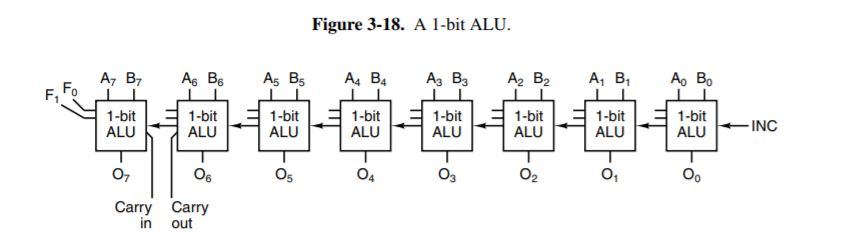
\includegraphics[width=1.00\textwidth]{8bit_ALU}
				\caption{8 ALU a 1 bit connesse fra loro}
			\end{figure}
			Circuiti come quelli mostrati nella figura soprastante, vengono chiamati \textbf{bit slices} che permettono ai progettisti di calcolatori di costruire ALU di larghezza arbitraria. \\
			Il segnale INC viene utilizzato solo per operazioni di addizione e permette di incrementare il risultato di 1, cioè $A + 1$ o $A + B + 1$ o $B + 1$.
			\section{Clock}
			Un \textbf{clock} è un circuito che emette una serie di impulsi di larghezza definita a intervalli di temporali costanti. L'intervallo temporale compreso tra le estremità di due impulsi consecutivi è detto \textbf{ciclo di clock}.
			\section{Memoria}
			La memoria è un componente essenziale di un calcolatore e viene utilizzata per conservare le istruzioni da eseguire e i dati. \\
			Verranno analizzati i componenti di un sistema di memoria, partendo dal livello delle porte logiche per capire come funziona e come sono combinate per formare memorie più complesse e capaci.
			\subsection{Latch SR}
			Per creare una memoria a 1 bit è necessario avere un circuito che sia in grado di memorizzare i valori di input. \\
			Questo è quello che fa il Latch SR, dove la S sta per \textbf{Set} e la R per \textbf{Reset}. \\
			Quindi, il Latch SR, ha appunto come input $S$ e $R$ e come output ha $Q$ e $\overline Q$. \\
			Il latch SR viene costruito con due porte NOR e l'uscita di queste è input dell'altra, cioè:
			\begin{figure}[H]
				\centering
				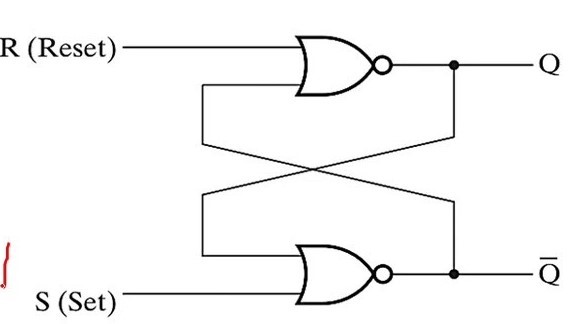
\includegraphics[width=0.75\textwidth]{latchSR}
				\caption{Circuito logico del latch SR}
			\end{figure}
			\begin{tabular}{cc|ccc}
				$\mathbf{S}$ & $\mathbf{R}$ & $\mathbf{Q}$ & $\mathbf{\overline Q}$ \\
				\hline
				0 & 0 & 1 & 0 & \multirow{2}{*}{Set state} \\
				1 & 0 & 1 & 0 & \\ 
				\hline
				0 & 0 & 0 & 1 & \multirow{2}{*}{Reset state}\\
				0 & 1 & 0 & 1 & \\
				\hline
				1 & 1 & 0 & 0 & Undefined state \\
			\end{tabular} \\
			Lo stato $S$ = 0 e $R$ = 0 è detto \textbf{stato di riposo} e mantiene in memoria il valore. \\
			Lo stato $S$ = 1 e $R$ = 1 è detto \textbf{stato d'indeterminazione}
			\subsection{Latch SR temporizzato}
			Spesso è preferibile che il latch non cambi di stato se non in specifici momenti. Perciò, si modifica il circuito del latch SR, aggiungendo un input, il clock, il cui valore è generalmente 0 e indipendentemente dal valore si $S$ e $R$ il valore generato dalle porte AND è 0, quando il clock vale 1, le porte AND non bloccano più i segnali e $S$ e $R$ dirigono lo stato del latch. \\
			Questo tipo di circuito è chiamato \textbf{latch SR temporizzato}.
			\begin{figure}[H]
				\centering
				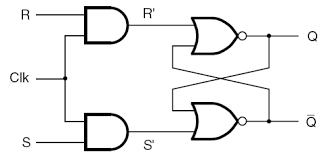
\includegraphics{latchSRtemp}
				\caption{Circuito logico del latch SR temporizzato}
			\end{figure}
			\subsection{Latch D temporizzato}
			Per evitare lo stato d'indeterminazione del latch SR, cioè dove $S=R=1$, si utilizza il \textbf{latch D temporizzato}, che presenta come input il segnale di clock e il valore $D$ che sta per $Data$. Gli input delle due porte AND sono il valore del clock, il cui funzionamento è analogo al circuito precedente, e il valore $D$ e $\overline D$, in questo modo non si verificherà mai la situazione $S=R=1$.
			\begin{figure}[H]
				\centering
				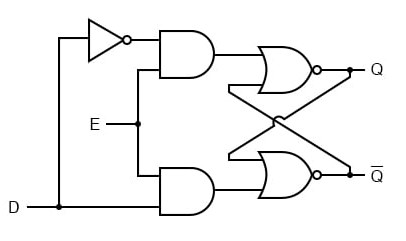
\includegraphics[width=0.63\textwidth]{latchD}
				\caption{Circuito logico del latch D}
			\end{figure}
			\subsection{Generatore di impulsi}
			\begin{figure}[H]
				\centering
				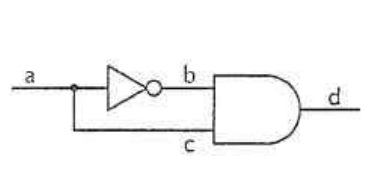
\includegraphics{generatore_impulsi}
				\caption{Circuito del generatore d'impulsi}
			\end{figure}
			A prima vista, questo circuito potrebbe confondere e potrebbe far pensare che il valore calcolato dalla porta AND sia sempre 0. \\
			Teoricamente funziona cosi, cioè genera sempre 0 come valore, praticamente non è cosi perchè il piccolissimo ritardo generato dalla porta NOT fa in modo che questo circuito per una frazione di secondo genera come valore 1. \\
			Questo circuito viene utilizzato nei Flip Flop.
			\subsection{Flip Flop}
			Il flip flop campiona e memorizza il valore di una linea in un particolare istante. Nei flip flop, infatti la transizione di stato non si verifica quando il clock vale 1, ma durante la transizione del clock da 0 a 1, cioè nel \textit{fronte di salita}, o durante la transizione da 1 a 0, cioè nel \textit{fronte di discesa}.\\
			Per campionare il valore di una linea durante la transizione del valore di clock, è necessario utilizzare appunto il generatore di impulsi che prende come ingresso il segnale di clock, in questo modo viene generato un impulso di lunghezza molto breve.
			\begin{figure}[H]
				\centering
				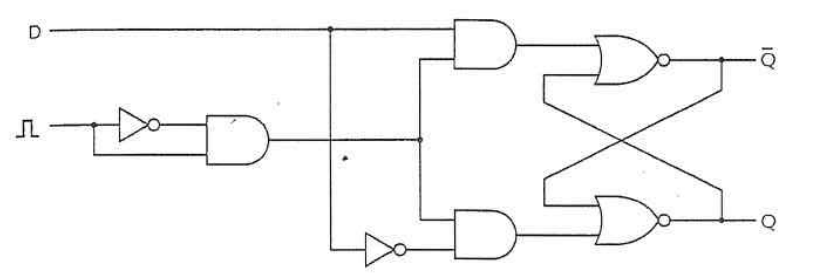
\includegraphics[width=1.0\textwidth]{FlipFlopD}
				\caption{Circuito del Flip Flop D}
			\end{figure}
			Come si può vedere, il circuito è molto simile a quello del latch D, con l'unica differenza che viene generato un impulso molto breve tramite il segnale di clock.
			\subsection{Registri}
			I Flip-Flop possono essere combinati per creare dei registri che memorizzano dati composti da più bit, ad esempio possiamo collegare 8 flip flop a 1 bit per formare un registro a 8 bit, come mostrato in figura:
			\begin{figure}[H]
				\centering
				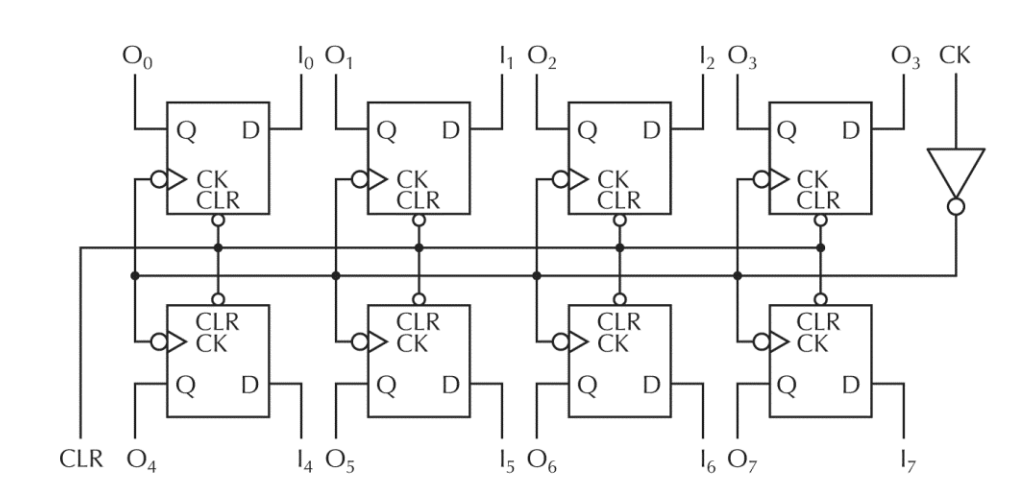
\includegraphics[width=1.00\textwidth]{8bit_register}
			\end{figure}
			Il registro riceve in ingresso un valore di 8 bit quando vi è una transizione del clock CK. Tutti gli 8 otto canali di cancellazione sono collegati fra loro, in modo che quando CLR va a 0 tutti i flip-flop sono forzati ad assumere valore 0. \\
			Il segnale CK viene invertito nella linea di input e viene invertito nuovamente in corrispondenza di ciascun flip-flop, perchè un segnale potrebbe non avere corrente sufficiente per pilotare tutti i flip-flop e quindi l'invertitore svolge il ruole di amplificatore.
			\subsection{Organizzazione della memoria}
			Fino ad ora abbiamo analizzato memorie di piccole dimensioni, per realizzarne altre di dimensione maggiore è necessario indirizzare singole parole, quindi c'è bisogno di un'organizzazione differente. Ad esempio:
			\begin{figure}[H]
				\centering
				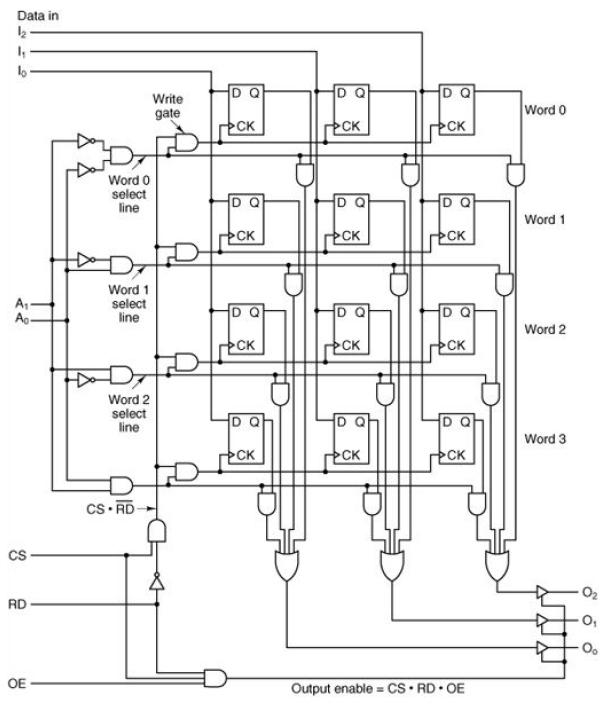
\includegraphics[width=0.75\textwidth]{12bit_memoria}
			\end{figure}
			Questa è una memoria con 4 parola a 3 bit e ciascuna operazione legge o scrive un'intera parola, una caratteristica notevole è che questo tipo di organizzazione può essere estesa a memorie di dimensioni maggiori. Il numero di parole è sempre una potenza di 2. \\
			Questa memoria di 12 bit necessita meno segnali a quelle di 8 bit viste precedentemente che utilizzavano 20 pin rispetto ai 13 utilizzati da quest'ultima, perchè a differenza dei registri, condividono un segnale di output.
			Il segnale RD vale 1 in caso di lettura e 0 nel caso di scrittura. Le due linee dell'indirizzo $A_0$ e $A_1$ devono essere impostate in modo da indicare quali delle 4 parole deve essere selezionata. In lettura le linee di input non vengono utilizzate e la parola viene resa disponibile sui segnali di output, in caso di scrittura avviene il contrario. \\
			A sinistra, in corrispondenza delle linee di indirizzo, troviamo 4 porte AND che formano un decodificatore che serve per scegliere la parola sulla quale operare. \\
			Quando l'operazione di scrittura è selezionata, l'output di questa porta guida tutti i segnali CK relativi alla parola selezionata, caricando i dati di input nei flip-flop che costituiscono la parola stessa. \\
			Quando viene attivata l'operazione di lettura, vengono disabilitate tutte le porte di scrittura. La linea per la selezione della parola scelta abilita la porta AND alla quale sono collegati i bit Q della parola selezionata, spedendo i dati alle porte OR. \\
			Anche se si potrebbe pensare di collegare le tre porte OR alle linee di output, è un approccio che si evita in quanto il chip avrebbe cercato di spedire in output i dati in caso di lettura e scrittura, forzando ogni linea ad assumere un certo valore e interferendo con i dati di input, per questo abbiamo bisogno di connettere le porte OR in caso di lettura e di disconnetterle in caso di scrittura. \\ 
			Quello di cui abbiamo bisogno è di un \textbf{buffer non invertente} che presenta un dato di input, un dato di output e un input di controllo, quando il controllo è alto il buffer funge da collegamento, quando è basso il circuito si comporta come un circuito aperto. \\
			Analogamente al buffer non invertente, esiste il \textbf{buffer invertente} che si comporta come un normale invertitore quando il controllo ha valore alto e disconnette l'output quando il controllo ha valore basso. \\
			I buffer inoltre amplificano il segnale e possono guidare più input allo stesso tempo e a volte vengono usati nei circuiti proprio per questo.
			\subsection{Chip di memoria}
			Per ampliare la memoria $4 \times 3$ vista prima ad una $4 \times 8$ basta aggiungere 5 colonne composte da 4 flip-flop ciascuna, aggiungere 5 linee di input e output. Se la si vuole estendere ad una memoria $8 \times 3$, basta aggiungere una nuova linea di indirizzo e 4 righe da 3 flip-flip ciascuna. \\
			Dato che la tecnologia dei circuiti integrati è adatta a realizzare chip con uno schema bidimensionale ripetuto, i chip di memoria sono un'applicazione ideale. Con l'avanzamento della tecnologia i numeri di bit all'interno di un chip aumentano sempre di più come dice la legge di Moore, non rendendo necessariamente obsoleti i chip con un numero di bit inferiore. \\
			Esempi di chip di memoria:
			\begin{figure}[H]
				\centering
				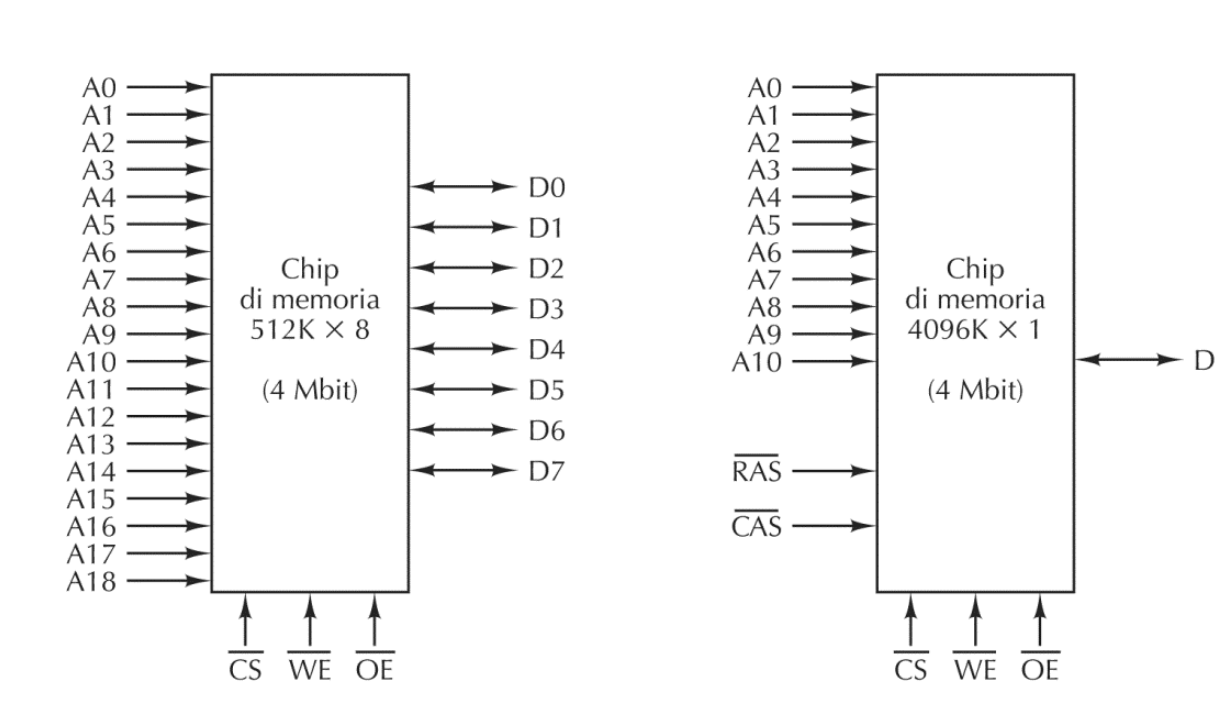
\includegraphics[width=1.00\textwidth]{chip_di_memoria}
				\caption{Chip di memoria a 4 bit}
			\end{figure}
			Su alcuni pin l'applicazione di un'alta tensione genera un'azione, su altri, invece, l'applicazione di una bassa tensione innesca un'azione. In generale si dice che un segnale è \textbf{asserito} per indicare che è impostato in modo da generare un'azione. \\
			I pin asseriti con valore basso sono identificati da una linea sopra il loro nome. L'opposto di è \textbf{negato} quando non succede nulla di particolare se i pin sono negati.
			\subsection{RAM e ROM}
			\textbf{RAM} \\
			Tutte le memorie analizzate fino ad ora possono essere sia lette che scritte. Le memorie di questo tipo sono chiamate \textbf{RAM}, Random Access Memory. \\
			Esistono due tipi di RAM: \textbf{statiche} e \textbf{dinamiche}. \\
			Le \textbf{RAM STATICHE, SRAM} sono costruite utilizzando circuiti simili ai flip-flop D e hanno la proprietà di mantenere il loro contenuto finchè vi è alimentazione. Le RAM statiche sono molto veloci e i loro tempi di accesso sono usualmente dell'ordine dei nanosecondi e per questo sono diffuse come memorie cache di secondo livello. \\
			Le \textbf{RAM DINAMICHE, DRAM} sono composte da un array di celle, ciascuna delle quali contiene un transistor e un piccolo condensatore che può essere caricato per memorizzare i valori 0 e 1. Dato che la carica elettrica tende a disperdersi occorre effettuare dei \textbf{refresh} di ciascun bit della RAM per evitare che i dati vadano persi.  Per via dei refresh le RAM dinamiche hanno un'interfaccia più complessa delle RAM statiche, però questo svantaggio è compensato dalla capacità offerta dalle RAM dinamiche. \\
			Le RAM dinamiche hanno molti bit per chip, cioè molta \textbf{densità}, per questo le memorie centrali sono sempre costruite utilizzando questo tipo di RAM che però sono più lente. Per questo si ricorre ad un uso combinato, si realizzano le cache con una RAM statica e la memoria centrale con la RAM dinamica. \\
			Esistono vari tipi di DRAM, la più antica è la DRAM \textbf{FPM} (Fast Page Mode) ancora utilizzata nei calcolatori più vecchi. Questa è stata sostituita dalla DRAM \textbf{EDO} (Extended Data Output) in cui un riferimento alla memoria può iniziare ancor prima che il precedente sia completo, aumentando la larghezza di banda della memoria. \\
			Con processori più veloci, c'era bisogno di memorie più veloci, per questo sono FPM e EDO sono stati sostituiti dalle \textbf{SDRAM}, dove la S sta per \textbf{Synchronus}, che è in parte statica e in parte dinamica ed è guidata dal clock principale del sistema, il vantaggio di queste è che il clock elimina la necessità dei segnali di controllo per specificare al chip quando deve rispondere. La CPU comunica alla memoria per quanti cicli deve funzionare e poi fa partire l'esecuzione. \\
			Dopo la SDRAM, si è passati alla SDRAM \textbf{DDR} (Double Data Rate), dove il chip produce un output sul fronte di salita del segnale di clock e uno sul fronte di discesa, raddoppiando il tasso di trasferimento dei dati. Le memoria DDR2 e DDR3 offrono prestazioni migliori delle DDR grazie ai bus più veloci. \\ \\
			\textbf{ROM} \\
			In molte applicazioni alcuni dati devono rimanere memorizzati anche quando viene tolta l'alimentazione, per questo sono state sviluppate le \textbf{ROM} che non possono essere modificate o cancellate. I dati sono inseriti durante la fabbricazione esponendo alla luce un materiale fotosensibile attraverso una maschera contenente il pattern di bit desiderato. L'unico modo per cambiare il programma consiste nella sostituzione dell'intero chip. \\
			Le memorie ROM, quindi, non sono flessibili e inoltre, passa molto tempo tra l'ordine e la ricezione di una ROM. Perciò sono state inventate le \textbf{PROM}, le ROM programmabili, che può essere programmata sul posto. \\
			Successivamente è stata prodotta la \textbf{EPROM}, la ROM programmabile cancellabile, esponendo la piccola lente al quarzo che si trova in essa a un'intensa luce ultravioletta. Per questo, le EPROM sono riutilizzabili e sono più economiche delle PROM. \\
			Il passo successivo sono le \textbf{EEPROM} cioè le ROM cancellabili elettricamente e queste sono anche riprogrammabili senza doverle rimuovere dal circuito. \\
			Le EEPROM però sono più piccole e più lente delle EPROM e sono utilizzate quando la proprietà di non volatilità è cruciale. \\
			Un tipo di EEPROM è la \textbf{memoria flash} che è cancellabile a blocchi e riscrivibile. \\ \\
			\textbf{FPGA} \\
			Gli \textbf{FPGA} (Field-programmable gate array) sono circuiti integrati che contengono una logica programmabile e permettono di formare un circuito logico arbitrario semplicemente caricando l'FPGA con i dati di configurazione appropriati. Il vantaggio principale di questi circuiti è la possibilità di costruire nuovi circuiti hardware in poche ore, senza aspettare mesi di fabbricazione dei circuiti integrati, che però, sono più vantaggiosi in termini di costi, velocità e consumo e proprio per questi vantaggi gli FPGA vengono utilizzati solo per la prototipazione e la progettazione di applicazioni su piccola scala. \\
			Il vantaggio principale degli FPGA è che si può costruire artigianalmente a casa in un'ora, mentre il più efficiente design completamente personalizzato deve essere fabbricato a partire dal silicio e questo potrebbe richiedere anche più di un mese.			
			\section{Chip della CPU e BUS}
			Tutte le CPU moderne sono contenute in unico chip, rendendo ben definita l'interazione con il resto del sistema. Ogni chip di CPU ha un insieme di pin attraverso il quale passano tutte le relative comunicazioni verso il mondo esterno. Alcuni pin spediscono i segnali della CPU, altri ricevono quelli del mondo esterno e altri fanno entrambe le cose. \\
			I pin di una CPU possono essere divisi in tre tipologie: indirizzi, dati e controlli. Questi pin poi sono collegati ai pin della memoria o dei dispositivi I/O tramite i bus. \\
			La CPU per prelevare un'istruzione ne imposta l'indirizzo sui suoi pin di indirizzamento e poi asserisce una o più linee di controllo per informare la memoria che vuole leggere una parola. La memoria poi risponde inviando la parola sui pin della CPU dedicati ai dati e segnalando che l'operazione è completata, così la CPU accetta la parola ed esegue l'istruzione. \\
			Due parametri che definiscono le prestazioni di una CPU sono il numero di pin d'indirizzo e quindi il numero di locazioni di memoria indirizzabili pari a $2^n$ con $n$ bit d'indirizzo e il secondo parametro è il numero di pin di dati cioè in un'unica operazione a CPU può leggere o scrivere una parola a $m$ bit se ha $m$ pin di dati. \\
			Come già detto precedentemente, la CPU è dotata di pin di controllo, i quali regolano il flusso e la temporizzazione dei dati da e verso la CPU, e possono essere utilizzati anche in vari altri modi. Tutte le CPU hanno pin per l'alimentazione, oltre a un segnale di clock e altri pin che variano da chip a chip. \\
			I pin di controllo, comunque, possono raggruppati in 6 categorie: 
			\begin{enumerate}
				\item \textbf{controllo del bus}: questi mandano sul bus dei segnali della CPU per notificare quando la CPU vuole compiere un'azione e la CPU utilizza questi pin per comunicare con il resto del sistema dicendo quali operazioni vuole eseguire;
				\item \textbf{interrupt}: questi sono degli input che giungono alla CPU dalle periferiche quando un dispositivo di I/O ha completato la propria operazione e asserisce un segnale su uno di questi pin in modo da intterompere la CPU e permetterle di utilizzare il dispositivo;
				\item \textbf{arbitraggio del bus}: questi sono necessari per regolare il traffico sul bus con l'obiettivo di evitare che due dispositivi cerchino di usarlo nello stesso momento. Anche la CPU deve fare richiesta per utilizzare un bus;
				\item \textbf{comunicazione con il coprocessore};
				\item \textbf{stato};
				\item \textbf{altro}.
			\end{enumerate}
			Oltre a questi segnali alcune CPU possono avere altri pin per altri scopi, come ricevere o fornire informazioni di stato o per garantire compatibilità con chip di I/O più vecchi.
			\begin{figure}[H]
				\centering
				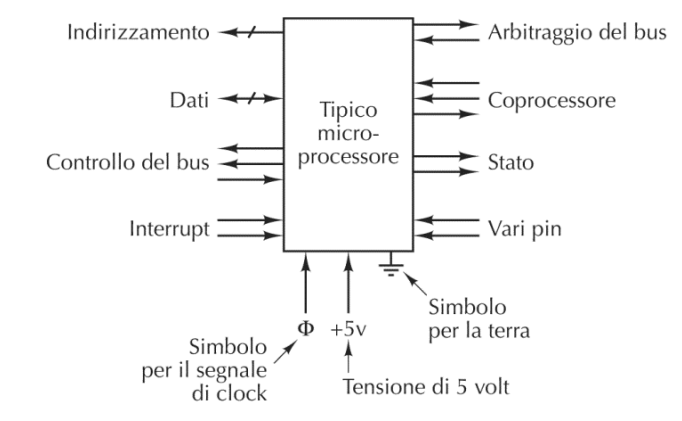
\includegraphics{chip_CPU}
				\caption{Le frecce indicano i segnali di input e di output. I trattini diagonali indicano pin multipli; per una specifica CPU un valore ne indica la quantità}
			\end{figure}
			 \paragraph{BUS del calcolatore}
			 Un \textbf{bus} è un collegamento elettrico che unisce diversi dispositivi. I bus possono essere classificati in base alla loro funzione, alcuni sono interni alla CPU per trasferire dati da e verso l'ALU, altri sono esterni e servono per collegarla con la memoria o con dispositivi I/O. \\
			 I primi PC avevano un unico bus esterno, il \textbf{bus di sistema} che era composto da 50 a 100 fili paralleli che si inserivano nella scheda madre e i connettori erano opportunamente distanziati per inserire memorie o schede I/O. Adesso i processori hanno un bus specifico per la CPU e la memoria e almeno un altro bus per le periferiche. ad esempio: 
			 \begin{figure}[H]
			 	\centering
			 	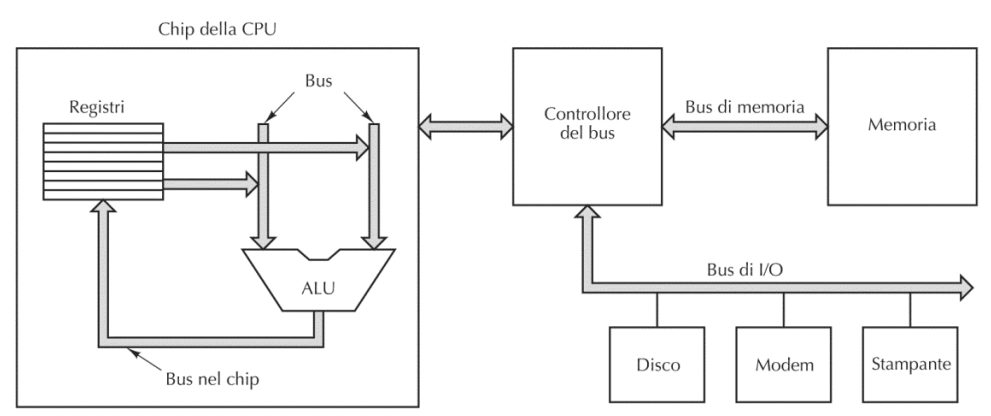
\includegraphics[width=1.00\textwidth]{bus_CPU}
			 	\caption{Sistema di un calcolate con più bus}
			 \end{figure} 
			 All'interno della CPU possono essere utilizzati i bus che si preferiscono, per i bus esterni, invece, bisogna definire delle regole di funzionamento che devono essere rispettate dai dispositivi collegati a loro, questo consente che anche schede progettate da altri produttori possono collegarsi al bus. L'insieme di queste regole viene chiamato \textbf{protocollo del bus}. Inoltre, devono essere definite le specifiche meccaniche ed elettriche in modo che le schede prodotte da terze parti abbiano dei connettori compatibili con quelli della scheda madre. \\
			 Esistono diversi bus ampiamente utilizzati, come: l'\textbf{Omnibus} utilizzato dal PDP-8, l'\textbf{Unibus} dal PDP-11, il \textbf{Multibus} dall'8086, il \textbf{Nubus} dal Macintosh, il \textbf{bus PCI} da molti PC, il \textbf{bus SCSI} da molti PC e workstation e l'\textbf{Universal Serial Bus} dai PC moderni. \\
			 Alcune periferiche che si collegano al bus sono attive e possono iniziare un trasferimento, i \textbf{master} mentre altri sono in attesa di una richiesta, gli \textbf{slave}. \\
			 Molto spesso i segnali digitali generati dalle periferiche sono tropo deboli per alimentare un bus, per questo molti master sono connessi al bus con un chip chiamato \textbf{driver del bus} che funge da amplificatore, mentre gli slave sono collegati attraverso un \textbf{ricevitore del bus}. Per le periferiche che possono essere sia master che slave si utilizza un chip chiamato \textbf{trasmettitore-ricevitore del bus}. Un'altra possibilità che permette di ottenere lo stesso risultato consiste nell'agganciare la periferica al bus tramite un \textbf{collettore aperto}. \\
			 Anche il bus ha i propri indirizzi, i propri dati e le proprie linee di controllo e non è necessario che vi sia una corrispondenza fra i pin del bus e quelli della CPU. 
			 \\ \\
			 \paragraph{Ampiezza del BUS} 
			 Un parametro da considerare durante la progettazione del bus è la sua ampiezza, maggiore è il nu ero di linee d'indirizzo di un bus, maggiore sarà la quantità di memoria che la CPU potrà indirizzare direttamente. \\
			 Il problema è che bus più larghi richiedono un numero maggiore di fili rispetto a quelli più stretti. Questo significa anche una maggiore occupazione di spazio e la necessità di utilizzare connettori più grandi. Dato che questi fattori rendono il bus più costoso è necesssario trovare un compromesso tra la dimensione massima di memoria e il costo del sistema. \\
			 Esistono due modi per aumentare la larghezza di banda dei dati su un bus: diminuire il periodo di clock oppure aumentare la larghezza dei dati sul bus. Un'altra soluzione è quella di aumentare la velocità del bus, ma questo poi causerebbe il \textbf{disallineamento del bus}, cioè i segnali su linee distinte viaggiano a velocità diverse. \\
			 Un altro problema quando si intende velocizzare il bus è la perdita della retrocompatibilità, infatti schede progettate con bus più lenti non funzioneranno con il nuovo bus. Perciò la tecnica più adottata è quella di aggiungere nuove linee di dati che però non genera un'architettura semplice e ordinata. \\
			 Per evitare il problema di bus troppo ampi spesso i progettisti usano un \textbf{bus multiplexato} dove vengono utilizzate un certo numero di linee, sia per le linee d'indirizzo e quelle dei dati. All'inizio di un operazione sul bus le linee sono utilizzate per gli indirizzi, mentre in seguito vengono usate per i dati. L'uso del bus multiplexato riduce l'ampiezza del bus ma rende il sistema più lento perchè con un normale bus, con le linee separate, è possibile spedire gli indirizzi e i dati allo stesso tempo.
			 \\ \\
			 \paragraph{Temporizzazione del BUS} 
			 I bus in base alla loro temporizzazione possono essere suddivisi in due categorie: i bus sincroni e bus asincroni.
			 
			 \subparagraph{Bus sincroni} 
 			 I bus sincroni hanno una linea regolata da un clock di sistema dove viaggia un'onda quadra con frequenza che da 5Mhz a 133Mhz e tutte le operazioni del bus richiedono un certo numero di questi cicli
			 \begin{figure}[H]
			 	\centering
			 	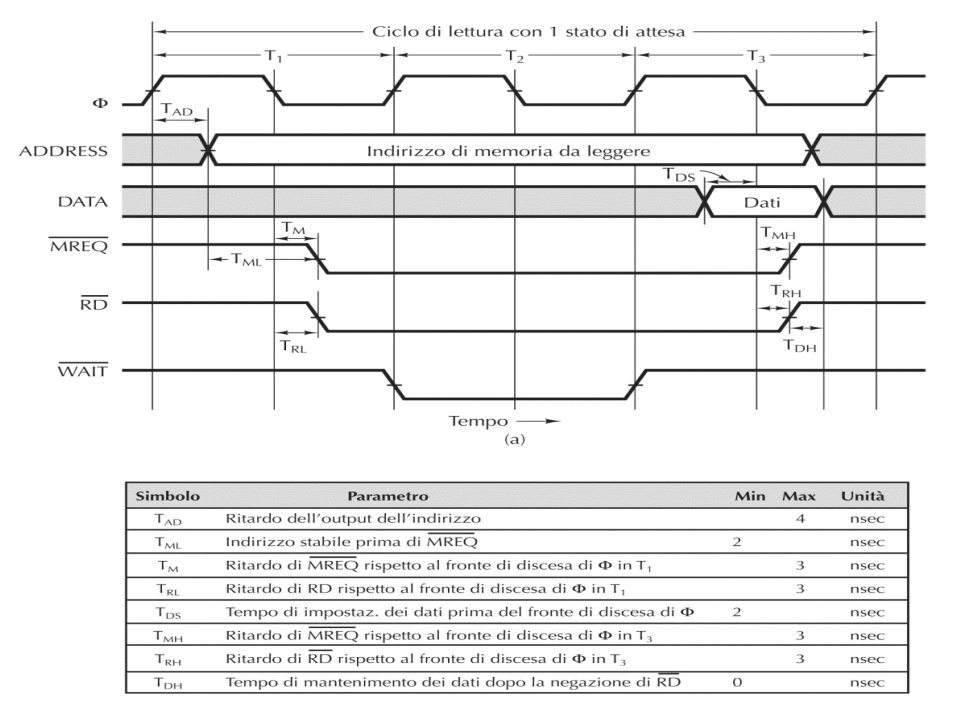
\includegraphics[width=1.00\textwidth]{bus_sincrono}
			 	\caption{Temporizzazione di una lettura su un bus sincrono con tabella che specifica alcuni tempi critici}
			 \end{figure}
			 Assumiamo che la lettura dalla memoria richieda 15 ns a partire dal momento in cui l'indirizzo è stabile. \\
			 Analizziamo la figura: \\
			 l'inizio di $T_1$ è definito dal fronte di salita del clock e a partire da $T_1$ la CPU fornisce l'indirizzo della parola sulle linee d'indirizzo e analogamente il contenuto delle linee dei dati non è significativo fino a $T_3$. \\
			 Dopo che le linee d'indirizzo hanno assunto i nuovi valori, vengono asserite $\overline{MREQ}$ e $\overline{RD}$, dove la prima indica che si sta per accedere alla memoria e la seconda è asserita per le lettura e negata per le scritture. Dato che la memoria impiega 15 ns dopo che l'indirizzo è stabile, non può fornire i dati richiesti durante $T_2$ e quindi all'inizio di $T_2$ asserisce $\overline{WAIT}$ per segnalare alla CPU di non aspettarla. \\
			 Questa operazione inserisce alcuni \textbf{stati di attesa} affinchè la memoria completi l'operazione e neghi $\overline{WAIT}$. All'inizio di $T_3$ la memoria nega $\overline{WAIT}$ perchè è sicuro che i dati sono disponibili nel corso del ciclo corrente. \\
			 Durante la prima metà di $T_3$ la memoria mette i dati sulle linee apposite e nel fronte di discesa di $T_3$ la CPU consulta le linee dei dati, memorizzando il valore in un suo registro. Dovendo leggere i dati la CPU nega $\overline{MREQ}$ e $\overline{RD}$. \\
			 Lavorare con i bus sincroni è facile per via dei loro intervalli temporali discreti però presentano alcuni problemi. \\
			 Innanzitutto, qualsiasi operazione si svolge in tempi multipli del clock del bus, quindi se una CPU e una memoria sono in grado di completare un trasferimento in 3,1 cicli sono obbligate ad allungare il tempo a 4 cicli. \\
			 Inoltre, una volta scelto un ciclo di bus e appositamente costruite le memorie e le schede di I/O è difficile trarre vantaggio dagli sviluppi della tecnologia che si verificheranno, cioè, se un bus sincrono ha un insieme eterogeneo di dispositivi, la velocità del bus deve essere regolata alla velocità della periferica più lenta. \\
			 Nonostante questo, la maggior parte dei bus è sincrona, in quanto è più facile da realizzare. 
			 \subparagraph{Bus asincroni}
			 I bus asincroni non hanno un clock di sistema e i cicli di bus possono avere una lunghezza qualsiasi e non devono essere necessariamente uguali nella comunicazione tra dispositivi. \\
			 \begin{figure}[H]
			 	\centering
			 	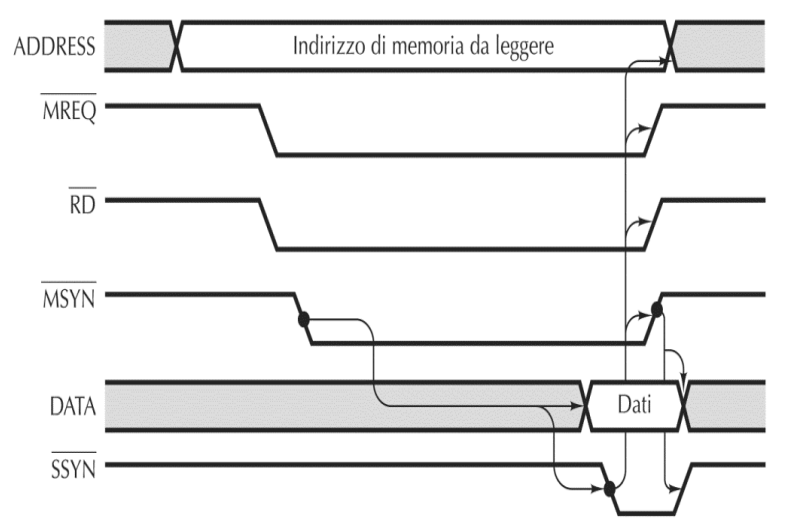
\includegraphics[width=1.00\textwidth]{bus_asincrono}
			 \end{figure}
			 Il master del bus, invece di legare ogni operazione al clock, dopo aver inserito l'indirizzo, $\overline{MREQ}, \overline{RD}$ e tutto ciò che è necessario, asserisce un segnale speciale chiamato $\overline{MSYN}$, Master SYNchronization. Quando lo slave vede questo segnale esegue il lavoro richiesto alla massima velocità possibile e una volta terminato il lavoro asserisce $\overline{SSYN}$, Slave SYNchronization. \\
			 Quando il master vede che $\overline{SSYN}$ è stato asserito, sa che i dati sono disponibili e quindi può memorizzarli e poi nega $\overline{MREQ}, \overline{RD}, \overline{MSYN}$ e quando lo slave vede che $\overline{MSYN}$ è negato nega $\overline{SSYN}$ e ora si attende il master successivo. \\
			 Notiamo quindi che l'asserzione di $\overline{MSYN}$ ha come effetto l'asserzione delle linee dei dati ed il fatto che lo slave asserisce $\overline{SSYN}$ e anche questa asserzione provoca l'asserzione di $\overline{MREQ}, \overline{RD}, \overline{MSYN}$ e l'asserzione di quest'ultimo provoca la negazione di $\overline{SSYN}$ e queste cause ed effetti nei diagrammi di temporizzazione è rappresentato con delle frecce. \\
			 Un insieme di segnali che coordina in questo modo due dispositivi con lo scopo di non farli interferire è chiamato \textbf{full handshake}: 
			 \begin{enumerate}
			 	\item $\overline{MSYN}$ è asserito;
			 	\item $\overline{SSYN}$ è asserito in risposta a $\overline{MSYN}$;
			 	\item $\overline{MSYN}$ è negato in risposta a $\overline{SSYN}$;
			 	\item $\overline{SSYN}$ è negato in risposta alla negazione di $\overline{MSYN}$.
			 \end{enumerate}
			 I full handshake non dipendono dalla temporizzazione ma ogni evento è causato da un evento precedente e non da un impulso di clock. \\
			 \paragraph{Arbitraggio del BUS} 
			 Finora ci è sempre capitata la situazione in cui la CPU era l'unico master del bus, ma non è cosi, anche i dispositivi I/O possono diventare master o anche i coprocessori e quindi nel caso in cui più dispositivi vogliono diventare master nello stesso istante c'è bisogno di una forma di \textbf{arbitraggio del bus} che può essere centralizzato o decentralizzato. 
			 \subparagraph{Arbitraggio centralizzato}
			 Analizziamo la seguente figura di una forma di arbitraggio centralizzato: 
			 \begin{figure}[H]
			 	\centering
			 	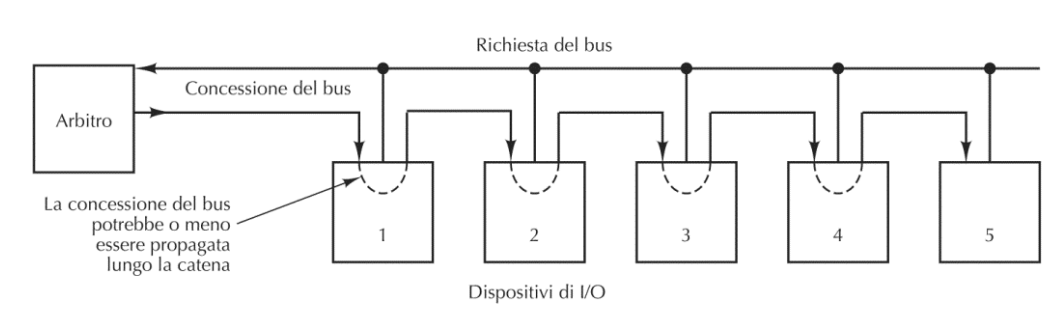
\includegraphics[width=1.00\textwidth]{daisy_chain}
			 \end{figure}
			 In questo schema un singolo arbitro del bus determina chi sarà il prossimo master. In molte CPU l'arbitro è integrato nel chip stesso, in altre, invece, bisogna utilizzare un chip separato. \\
			 Il bus contiene un'unica richiesta OR-cablata che in qualsiasi momento può essere asserita da uno o più dispositivi. L'arbitro ha solo la capacità di distinguere se c'è stata o meno una richiesta. \\
			 Quando l'arbitro vede una richiesta di utilizzo del bus, lo concede asserendo la linea per la concessione del bus. A questa linea sono collegati in serie tutti i dispositivi I/O e quando il dispositivo più vicino all'arbitro vede la concessione, controlla se ne ha fatto richiesta, in caso affermativo se ne impossessa, in caso negativo, propaga la concessione sulla linea in direzione del prossimo dispositivo che effettuerà la stessa procedura. Questo schema è chiamato \textbf{collegamento a festone} o \textbf{daisy chaining}. \\
			 Molti bus, per aggirare il fatto che le priorità sono implicitamente definita in base alla distanza dall'arbitro, definiscono dei livelli di priorità e per ciascun dispositivo esiste una linea per effettuare la richiesta e una per segnalare la concessione, come in figura. 
			 \begin{figure}[H]
			 	\centering
			 	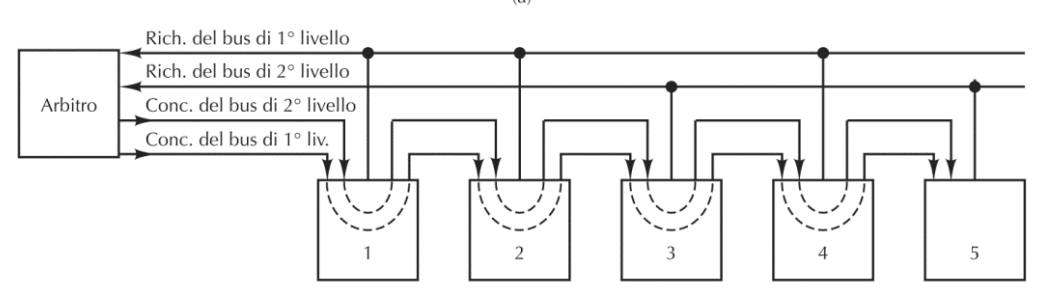
\includegraphics[width=1.00\textwidth]{arbitro_centr_2livelli}
			 \end{figure}
			 A ciascun dispositivo viene assegnato un livello per la richiesta del bus, a quelli per cui la temporizzazione è più critica vengono assegnate priorità più alte. Se in uno stesso momento ci sono richieste di livelli di priorità diversi l'arbitro concede il bus a un dispositivo di priorità più elevata; fra quelli con stessa priorità si adotta la strategia del collegamento a festone. \\
			 Alcuni arbitri hanno una terza linea che viene asserita da un dispositivo nel momento in cui accetta una concessione e si impadronisce del bus. Subito dopo aver asserito questa linea di conferma, il dispositivo può negare le linee di richiesta e di concessione così altri dispositivi possono richiedere il bus mentre il primo lo sta ancora utilizzando e nel momento in cui termina il master successivo è già stato selezionato. \\
			 Questo schema prevede maggiori componenti logici ma c'è un miglior utilizzo dei cicli di bus. \\
			 Nei sistemi in cui la memoria è collegata al bus principale e la CPU deve competere con i dispositivi I/O ad ogni ciclo, alla CPU viene assegnata priorità più bassa così da utilizzare il bus quando nessun altro lo vuole e anche perchè i dispositivi di I/O devono acquisire il bus molto velocemente per non perdere i dati. \\
			 
			 \subparagraph{Arbitraggio decentralizzato}
			 Un'altra soluzione è la decentralizzazione dell'arbitraggio del bus. Ad esempio, un calcolatore potrebbe avere 16 linee di richiesta, ciascuna con la propria priorità e quando un dispositivo vuole utilizzare il bus asserisce la linea di richiesta. Tutti i dispositivi monitorano tutte le linee di richiesta in modo che alla fine di ogni ciclo di bus ognuno di loro può sapere se ne aveva fatto richiesta e se aveva priorità più elevata e quindi se può utilizzare il bus. Questo richiede più linee di bus ma evita il costo dell'arbitro e un altro limite è che il numero di dispositivi deve essere pari a quello delle linee del bus. \\
			 Un altro tipo di decentralizzazione del bus, utilizza solamente tre linee: 
			 \begin{figure}[H]
			 	\centering
			 	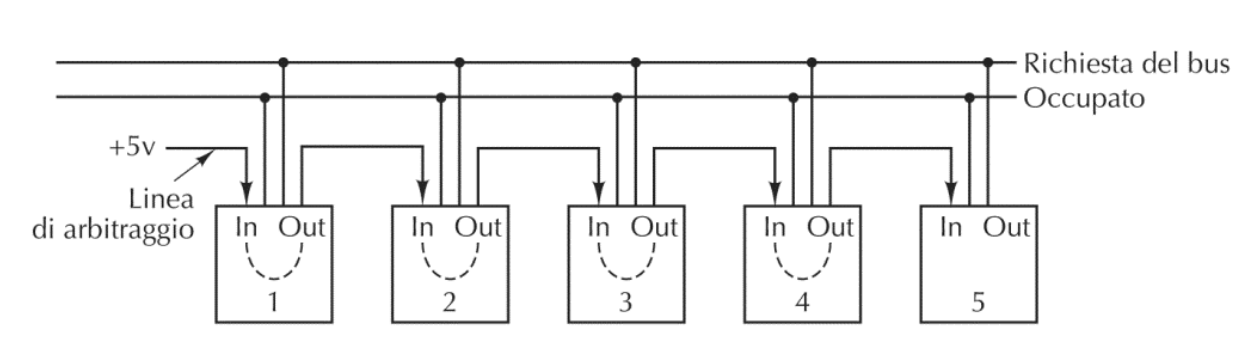
\includegraphics[width=1.00\textwidth]{bus_decentralizzato}
			 \end{figure}
			 La prima linea del bus è una linea OR-cablata per effettuare le richieste al bus. La seconda linea è chiamata BUSY ed è asserita dal master corrente, la terza è utilizzata per arbitrare il bus ed è un collegamento a festone tra i dispositivi. \\
			 Quando nessun dispositivo richiede al bus la linea di arbitraggio, che è asserita, viene propagata verso tutti i dispositivi. Per acquisire i bus un dispositivo deve controllare se il bus è inattivo e se il segnale dell'arbitraggio che sta ricevendo, IN, è asserito, in caso contrario non può diventare master e nega OUT. Se IN è asserito, il dispositivo nega OUT in modo che il dispositivo successivo veda IN negato e neghi anche lui il proprio OUT e così faranno tutti i dispositivi e solo uno rimarrà con IN asserito e OUT negato e diventerà il master del bus, asserirà BUSY e OUT e inzierà il trasferimento. 
			 \paragraph{Operazioni del BUS} 
			 Di solito viene trasferita una parola alla volta durante le operazioni in memoria. Tuttavia, quando si utilizza la cache, è meglio prelevare in una volta sola un'intera linea di cache, perchè, spesso, i trasferimenti in blocchi possono essere effettuati in modo più efficiente rispetto a una sequenza di trasferimenti individuali. All'inizio della lettura di un blocco il master del bus comunica allo slave quante parole devono essere trasferite inserendo il conteggio delle parole sulle linee dei dati. Lo slave genera in output a ogni ciclo una nuova parola finchè il contatore non si sia esaurito. \\
			 Esistono anche altri tipi di cicli di bus. Per esempio su un sistema multiprocessore con due o più CPU sullo stesso bus è necessario assicurarsi che soltanto una CPU utilizzi delle strutture dati critiche della memoria. Una soluzione consiste nell'avere in memoria una variabile che vale 0 quando nessuna CPU sta utilizzando la struttura dati e 1 quando è in uso. Se una CPU vuole acquisire accesso alla struttura dati deve leggere il valore della variabile e settarla a 1, se vale 0. Può capitare, però, che le CPU, leggano la variabile nello stesso istante e quindi entrambe leggeranno che la variabile vale 0 e le setteranno a 1 pensando che di essere l'unica CPU che sta utilizzando la struttura dati.\\
			 Per evitare questo, i sistemi multiprocessore hanno uno speciale ciclo di bus \textbf{leggi-modifica-scrivi} che consente a una qualsiasi CPU d leggere, analizzare e riscrivere una parola in memoria senza rilasciare il bus. In questo modo nessun'altra CPU interferirà. \\
			 Un'altra operazione importante serve a \textbf{gestire gli interrupt}. Quando la CPU ordina a un dispositivo I/O di effettuare un'operazione si aspetta un interrupt a fine operazione e per segnalare questi interrupt si utilizza il bus. \\
			 Visto che più dispositivi potrebbero voler generare un interrupt nello stesso momento, si assegna una priorità ai dispositivi e si utilizza un arbitro centralizzato per dare priorità al dispositivo per cui la temporizzazione è più critica. Nei chip basati su processori Intel il chipset incorpora il controllore di interrupt 8259A: 
			 \begin{figure}[H]
			 	\centering
			 	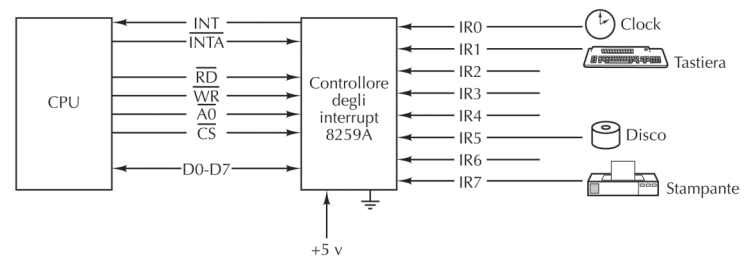
\includegraphics[width=1.00\textwidth]{8259A}
			 \end{figure} 
			 Questo chip ha 8 input IR, Interrupt Request, con i quali si possono collegare fino a 8 dispositivi I/O e quando un dispositivo vuole causare un interrupt asserisce la propria linea di input. Quando uno o più input sono asseriti, il chip asserisce INT, INTerrupt, che pilota il pin di interrupt sulla CPU, quando la CPU è pronta per  gestire l'interrupt spedisce un impulso su INTA, INTerrupt Acknowledge, a questo punto il chip deve specificare quale input ha causato l'interrupt generando in output il suo numero sul bus dei dati. L'hardware della CPU utilizza quel numero come indice all'interno di una tabella, \textbf{vettore di interrupt}, per cercare l'indirizzo della procedura da eseguire per poter gestire l'interrupt.
			 Il chip ha al suo interno vari registri che la CPU può utilizzare e i pin $\overleftarrow{RD}, \overleftarrow{WR}, \overline{CS}\ e \ \overline{AD}$. Quando il software ha gestito l'interrupt ed è pronto per accettarne uno nuovo scrive un codice speciale all'interno di uno di questi registri. \\
			 Quando sono presenti più di 8 dispositivi di I/O si possono utilizzare a cascata più chip 8259A, come il chip Intel ICH10, incorpora due chip 8259A, quindi ICH10 dispone di 15 interrupt esterni e non 16 perchè un interrupt viene utilizzato per connettere in cascata il secondo 8259A al primo.
			 \section{Interfacce}
			 Le interfacce I/O rappresentano la modalità con la quale il calcolatore comunica con il mondo esterno. 
			 \subsection{Interfacce di I/O}
			 Dei chip molto comuni sono gli UART, gli USART, i controllori dei dischi e i PIO. Una \textbf{UART}, Universal Asynchronous Receiver Transmitter, è un'interfaccia che può leggere un byte da un bus di dati e generarlo in output, bit per bit, su una linea seriale per un terminale, oppure può ricevere input da un terminale. Una \textbf{USART}, Universal Synchronous Asynchronous Receiver Transmitters, possono gestire trasmissioni sincrone, oltre a supportare le funzionalità dell'UART. Dato che le interfacce UART hanno perso di importanza, analizzeremo le interfacce PIO come chip di I/O.
			 \paragraph{Interfacce PIO}
			 Un interfaccia \textbf{PIO}, Parallel Input/Output, può essere rappresentata nel seguente modo:
			 \begin{figure}[H]
			 	\centering
			 	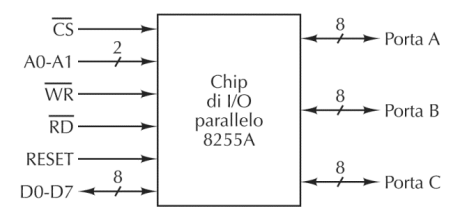
\includegraphics[width=1.00\textwidth]{Interfaccia_PIO}
			 \end{figure}
			 In questo caso, il chip contiene 24 linee di I/O che possono collegare qualsiasi interfaccia di dispositivo digitale e il programma della CPU può scrivere 0 o 1 su ogni linea, oppure può leggere in input lo stato di ogni linea. \\
			 L'interfaccia PIO viene usata spesso nei sistemi integrati e viene configurata grazie a un registro di configurazione a 3 bit che specifica se le 3 porte delle linee di input devono essere utilizzate per un segnale digitale in ingresso o in uscita. \\
			 A ciascuna porta è associato un registro latch a 8 bit e per impostare le linee su una porta, la CPU scrive un numero a 8 bit nel registro corrispondente che rimarrà sulla linea di output fino a quando il registro non viene riscritto. \\
			 Per utilizzare la porta in input, la CPU legge semplicemente il registro corrispondente. \\
			 Inoltre, è possibile anche utilizzare l'handshaking con dispositivi esterni. Per spedire un output verso un dispositivo che non è sempre pronto ad accettare i dati, l'interfaccia PIO li rende disponibili su una porta di output e attende che il dispositivo restituisce un segnale per indicare che ha accettato i dati e ne desidera altri. \\
			 Oltre alle 24 linee di I/O, il chip cdisponde di otto linee che lo connettono direttamente al bus dati, una linea per la selezione del chip, le linee per la lettura e la scrittura, due linee d'indirizzo e una linea per resettare il chip. La linea CS permette di combinare più interfacce PIO a 24 bit per formare un'interfaccia PIO più grande.
			 \paragraph{Decodifica dell'indirizzo}
			 Consideriamo un calcolatore a 16 bit composto da una CPU, una EPROM per il programma da 2KB $\times$ 8 byte, una RAM per i dati da 2KB $\times$ 8 byte e un'interfaccia PIO. \\
			 L'interfaccia PIO può essere selezionata come un vero dispositivo I/O o come parte della memoria. Se scegliamo di usarla come parte di memoria, quindi dell'\textbf{I/O mappato in memoria}, dobbiamo assegnargli 4 byte dello spazio di memoria, necessari per indirizzare le tre porte e il registro di controllo. \\
			 \begin{figure}[H]
			 	\centering
			 	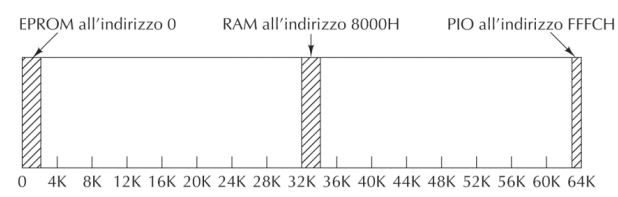
\includegraphics[width=1.00\textwidth]{PIO_memoria}
			 \end{figure}
			 Dato che lo spazio degli indirizzi è 64 KB dobbiamo scegliere come collocare i tre dispositivi. Questa scelta dal punto di vista del programmatore non cambia nulla, dal punto di vista dell'interfaccia sì, perchè se avessimo scelto di indirizzare il chip PIO mediante lo spazio di I/O non ci sarebbe stato bisogno di alcun indirizzo di memoria. \\
			 Usando l'assegnamento degli indirizzi come quello in figura, gli indirizzi di memoria del tipo 0000xxxxxxxxxxx cadono nella EPROM. La selezione del chip della EPROM potrebbe essere collegata a un comparatore di 5 bit con input impostato a 00000, oppure, si può usare una porta OR a cinque ingressi collegati alle linee d'indirizzo che vanno da A11 a A15, se tutte queste valgono 0 allora l'output sarà 0, questo approccio è chiamato \textbf{full-addesss decoding}:
			 \begin{figure}[H]
			 	\centering
			 	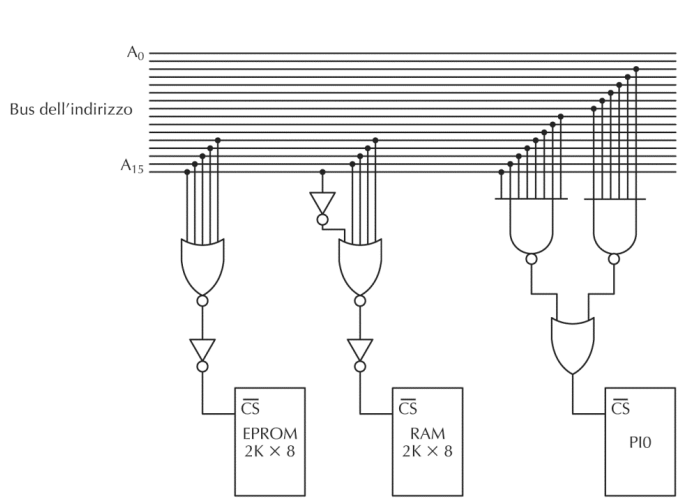
\includegraphics[width=1.00\textwidth]{full_address_decoding}
			 \end{figure}
			 Questo approccio può essere usato anche per la RAM con indirizzi della forma 10000xxxxxxxxxxx, mentre per gli indirizzi del chip PIO è più complicato perchè gli indirizzi sono della forma 111111111xx. \\
			 Se il calcolatore è veramente composto dalla CPU, da due chip di memoria e dal chip PIO, allora gli indirizzi li possiamo decodificare in modo più semplice, perchè sappiamo che gli indirizzi della EPROM hanno uno 0 nel bit più significativo, A15 e quindi possiamo collegare $\overline{CS}$ direttamente ad esso. \\
			 Per la RAM, dobbiamo decodificare due bit, 10, e per il chip PIO, analogamente dobbiamo decodificare i bit 11.  \\
			 Questa è chiamata \textbf{decodifica parziale dell'indirizzo}: 
			 \begin{figure}[H]
			 	\centering
			 	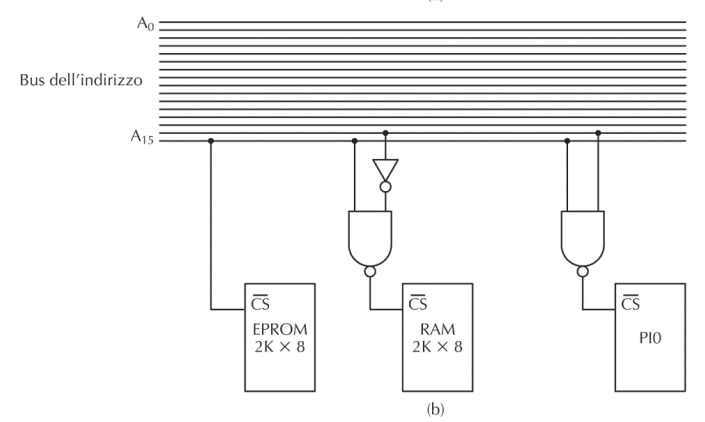
\includegraphics[width=1.00\textwidth]{decodifica_parziale}
			 \end{figure}
		\chapter{Espressioni logiche e mappe di Karnugh}
			\section{Forma normale disgiuntiva e congiuntiva}
			\begin{itemize}
				\item Un'espressione logica è detta in \textbf{\textit{forma normale disgiuntiva}} o \textit{DNF}(Disjuncitive normal form) o \textit{in prima forma canonica} se è una disgiunzione di clausole, dove ogni clausola è una congiunzione di letterali, quindi: 
				\[
				AB + B\overline{C} + A\overline{B}C
				\]
				\item Un'espressione logica è detta in \textbf{\textit{forma normale congiuntiva}} o \textit{CNF}(Conjunctive normal form) o \textit{seconda forma canonica} se è una congiunzione di clausole, dove ogni clausola è una disgiunzione di letterali, quindi: 
				\[
				(A + B)(B + \overline{C})(A + \overline{B} + C)
				\]
			\end{itemize}
			Qualunque espressione logica può essere tradotta in DNF o CNF.
			\section{Ricostruire un'espressione logica}
			Se si ha a disposizione una funzione logica arbitraria, è immediato ricavarne la tabella di verità e il circuito corrispondente, oppure è immediato risalire alla funzione logica tramite il circuito. Ma come si può risalire dalla tabella di verità alla funzione logica? \\
			Per fare questo ci sono diversi modi come la \textbf{\textit{ riscrittura in somma di mintermini}}, la \textbf{\textit{riscrittura in prodotto di maxtermini}}, il \textbf{\textit{teorema di Shannon}} e le \textbf{\textit{mappe di Karnaugh}}.
				\subsection{Mintermini e maxtermini}
					\begin{itemize}
						\item  Tramite la procedura della \textbf{\textit{riscrittura in somma di mintermini}} si ricava un'espressione logica che sarà espressa in \textbf{forma normale disgiuntiva}. \\
						Un \textbf{mintermine} è una funzione booleana che assume il valore vero in corrispondenza di un'unica configurazione di variabili booleane indipendenti.
						\item Tramite la procedura della \textbf{\textit{riscrittura in prodotto di maxtermini}} si ottiene un'espressione espressa in \textbf{forma normale congiuntiva}. \\
						Un \textbf{maxtermine} è una funzione boolena che assume valore falso di un'unica configurazione di variabili booleane indipendenti
					\end{itemize}
					Le due scritture si equivalgono. \\
					Per ciascuna combinazione di input di una tabella di verità è possibile ricavarne il mintermine e il maxtermine, ad esempio: \\ \\
					\begin{tabular}{c|c|c|c|c}
						$A$ & $B$ & $C$ & \textbf{Mintermine} & \textbf{Maxtermine} \\
						\hline
						0 & 0 & 0 & $\overline{A}\ \overline{B}\ \overline{C}$ & $A + B + C$ \\
						0 & 0 & 1 & $\overline{A}\ \overline{B}\ C$ & $A + B + \overline{C}$ \\
						0 & 1 & 0 & $\overline{A}\ B\ \overline{C}$ & $A + \overline{B} + C$ \\
						0 & 1 & 1 & $\overline{A}\ B\ C$ & $A + \overline{B} + \overline{C}$ \\
						1 & 0 & 0 & $A\ \overline{B}\ \overline{C}$ & $\overline{A} + B + C$ \\
						1 & 0 & 1 & $\overline{A}\ B\ \overline{C}$ & $\overline{A} + B + \overline{C}$ \\
						1 & 1 & 0 & $A\ B\ \overline{C}$ & $\overline{A} + \overline{B} + C$ \\
						1 & 1 & 1 & $A\ B\ C$ & $\overline{A} + \overline{B} + \overline{C}$ \\
					\end{tabular} \\ \\
					Ciascun mintermine si oittiene come prodotto delle singole variabili booleane, associando:
					\begin{itemize}
						\item la variabile booleana quando il valore è 1;
						\item la variabile booleana negata quando il valore è 0;
					\end{itemize}
					Per il maxtermine avviene l'inverso, e ogni mintermine è la negazione del maxtermine e viceversa, per via delle leggi di Demorgan. \\
					Una qualsiasi funzione booleana può essere riscritta in \textbf{\textit{\color{red}somma di mintermini}} sommando tutti i mintermini delle combinazioni dove la funzione assume valore 1.\\ \\
					\begin{tabular}{c|c|c|c}
						$A$ & $B$ & $C$ & \textbf{\textit{f}} \\
						\hline
						0 & 0 & 0 & 1 \\
						0 & 0 & 1 & 0 \\
						0 & 1 & 0 & 1 \\
						0 & 1 & 1 & 1 \\
						1 & 0 & 0 & 0 \\
						1 & 0 & 1 & 0 \\
						1 & 1 & 0 & 1 \\
						1 & 1 & 1 & 1 \\
					\end{tabular} \\ \\
					Quindi: 
					\[
					f = \overline{A}\cdot\overline{B}\cdot\overline{C} + \overline{A}\cdot B \cdot\overline{C} + \overline{A}\cdot B \cdot C + A \cdot B \cdot\overline{C} + A \cdot B \cdot C 
					\]
				Per riscriverla in \textbf{\textit{\color{red}prodotto di maxtermini}} bisogna moltiplicare tutti i maxtermini della combinazioni dove la funzione assume valore 0, quindi nel caso della funzione di prima:
				\[
				f=(A + B + \overline{C})(\overline{A} + B + C)(\overline{A} + B + \overline{C})
				\]
				Generalmente si preferisce la scrittura in \textbf{somma di mintermini}, l'espressione che se ne ricava però \textbf{non è detto che sia minima} e quindi si deve provare a semplificarla.
				\subsection{Semplificare un'espressione logica}
				Semplificare un'espressione consente dei vantaggi:
				\begin{itemize}
					\item gestione algebrica più semplice, perchè ci sono meno porte e il circuito è più semplice
					\item in termini di velocità, con meno porte il circuito è più veloce
					\item in termini di costi, ci sono meno spese se le porte sono di meno
				\end{itemize}
				Nel caso di prima dove $f$ era:
				\[
				f = \overline{A}\cdot\overline{B}\cdot\overline{C} + \overline{A}\cdot B \cdot\overline{C} + \overline{A}\cdot B \cdot C + A \cdot B \cdot\overline{C} + A \cdot B \cdot C 
				\]
				$=\overline{A}\cdot\overline{B}\cdot\overline{C} + \overline{A}B(C + \overline{C}) + AB(\overline{C} + C)$ \\
				Ora possiamo applicare la complementazione forma OR di $\overline{C} + C$ che equivale a 1 e quindi: \\
				$=\overline{A}\ \overline{B}\ \overline{C} + \overline{A}B + AB$ \\
				$=\overline{A}\ \overline{B}\ \overline{C} + B(\overline{A} + A)$ \\
				$=\overline{A}\ \overline{B}\ \overline{C} + B$ \\
				Applicando la seconda legge di assorbimento forma OR, si ottiene: \\
				$=\overline{A}\ \overline{C} + B$
				\subsection{Teorema di Shannon}
				Il \textbf{\textit{teorema di Shannon}}, enunciato prima da George Boole, consente di scomporre una funzione booleana complessa in funzioni più semplici. \\
				Data una funzione $f$ in $n$ variabili, si ha che:
				\[
				f(v_1, v_2, ..., v_n) = v_1 \cdot f(1, v_2, ..., v_n) + \overline{v_1} \cdot f(0, v_2, ..., v_n) 
				\]
				La funzione complessa composta in partenza da $n$ variabili viene trasformata in una somma di due prodotti, aventi una funzione di $n - 1$ variabili. \\
				Applicare il teorema di Shannon su tutte le variabili, con tutte le sue semplificazioni, ci riporta alla somma di mintermini della funzione. \\
				Vedere poi il pdf per degli esempi concreti.
				\subsection{Mappa di Karnaugh}
				La mappa di Karnaugh è uno strumento che consente di ricavare, partendo dalla tavola di verità, la sua \textbf{espressione minima}. \\
				Il metodo della mappa di Karnaugh si basa sul metodo della somma di mintermini, ma le espressioni vengono semplificate direttamente, se il metodo viene applicato bene e quindi facendo i raggruppamenti migliori, si ricaverà l'espressione minima altrimenti si ricava un'espressione semplificabile. \\
				Questo metodo è efficace nei casi di funzione a 4 variabili, gestibili a 5 e 6 ma difficilmente applicabile a funzioni a più di 6 variabili. \\
				La mappa di Karnugh opera in tre fasi:
				\begin{enumerate}
					\item costruzione della/e mappe
					\item scelta dei raggruppamenti
					\item generazione degli implicanti e dell'espressione finale
				\end{enumerate}
				\begin{karnaugh-map}(label=corner)[4][4][1][B][A][D][C]
					
				\end{karnaugh-map} \\
				Questo è un esempio della mappa di Karnaugh, le variabili sono disposte lungo il lato superiore e il lato sinistro della tabella, ci sono massimo due variabili per lato, se c'è una variabile, i lati vengono divisi in due parti, se ce ne sono 2 i lati vengono divisi in 4 parti.
				\\
				Si nota che la configurazione per la doppia variabile non è: \textbf{00-01-10-11} ma è: \textbf{00-01-11-10}, questa prende il nome di \textbf{codifica di Gray} e si utilizza quando per passare da una casella all'altra cambia il valore di una sola variabile e quindi c'è la variazione di un solo bit.
				\\ \\
				\textbf{\color{red}Scelta dei raggruppamenti} \\
				Per raggruppare le celle della mappa di Karnugh dove il valore 1 bisogna rispettare delle condizioni:
				\begin{enumerate}
					\item si possono raggruppare solo elementi tra celle adiacenti orizzontalmente o verticalmente
					\item i raggruppamenti non devono contenere celle con valore 0
					\item si possono raggruppare solo elementi in rettangoli o quadrati
					\item il numero di celle di ciascun raggruppamento deve essere una potenza di 2
					\item tutte le celle con il valore 1 devono essere contenuto \textbf{almeno} in un raggruppamento
				\end{enumerate}
				I raggruppamenti di $2^k$ elementi prendono il nome di \textbf{\textit{k-cubi}} \\
				La griglia è da considerarsi come un piano, bensì come un \textbf{toro}, pertanto i raggruppamenti possono attraversa i bordi della mappa sia verticalmente che orizzontalmente, passando da un lato a quello opposto. \\
				
				\begin{tabular}{c|c|c|c|c}
					$A$ & $B$ & $C$ & $D$ & $f$ \\
					\hline
					0 & 0 & 0 & 0 & 0 \\
					0 & 0 & 0 & 1 & 1 \\
					0 & 0 & 1 & 0 & 1 \\
					0 & 0 & 1 & 1 & 1 \\
					0 & 1 & 0 & 0 & 0 \\
					0 & 1 & 0 & 1 & 1 \\
					0 & 1 & 1 & 0 & 0 \\
					0 & 1 & 1 & 1 & 1 \\
					1 & 0 & 0 & 0 & 0 \\
					1 & 0 & 0 & 1 & 0 \\
					1 & 0 & 1 & 0 & 1 \\
					1 & 0 & 1 & 1 & 1 \\
					1 & 1 & 0 & 0 & 1 \\
					1 & 1 & 0 & 1 & 0 \\
					1 & 1 & 1 & 0 & 0 \\
					1 & 1 & 1 & 1 & 1 \\
				\end{tabular} \\ \\
				Prendendo questa tavola di verità, si riportano nella mappa di Karnaugh i mintermini e seguono degli esempi di raggruppamenti validi: \\ 
				\begin{karnaugh-map}(label=corner)[4][4][1][B][A][D][C]
					\minterms{3, 4, 5, 12, 13, 14, 15, 8, 10}
					\implicant{4}{13}
					\implicant{12}{14}
					\implicant{3}{3}
					\implicantedge{8}{8}{10}{10}
				\end{karnaugh-map} \\
				L'espressione finale risultante dalla mappa di Karnaugh sarà una \textbf{somma di implicanti:}
				\[
				f = I_1 + I_2 + \cdots + I_n
				\]
				Ciascun implicante è dato dal raggruppamento individuato. \\
				Nell'esempio precedente gli implicanti sono: \\
				$\mathbf{\color{red}I_1} = \overline{A}D$, notiamo che la $B$ e la $C$ sono state escluse perchè il loro valore cambia. \\
				$\mathbf{\color{green}I_2} = CD$, anche qui $A$ e $B$ cambiano di valore e quindi vengono esclusi. \\
				$\mathbf{\color{blue}I_3} = \overline{B}C\overline{D}$, anche qui la $A$ cambia valore. \\
				$\mathbf{\color{yellow}I_4} = AB\overline{C}\ \overline{D}$ \\
				Quindi: $f = \overline{A}D + CD + \overline{B}C\overline{D} + AB\overline{C}\ \overline{D}$.  \\
				In questo esempio ogni implicante è \textbf{primo} cioè che non implica un altro implicante, vedere il pdf per degli esempi di implicanti non primi. \\ \\
				In una funzione booleana è possibile avere delle configurazioni il cui output, per diverse ragioni, non ci interessa. Questa condizione prende il nome di \textbf{condizione di indifferenza}. Queste condizioni sono generalmente indicate con la lettera greca phi $\phi$ che idealmente rappresenta uno 0 e un 1 sovrapposti, ma anche con X, $\Delta$, *, ... \\
				Queste condizioni rappresentano un \textbf{jolly} e verranno considerate se aiutano a costituire un raggruppamento o a costituire un raggruppamento migliore, se non forniscono alcun contributo non vengono considerate, ad esempio: 
				\begin{karnaugh-map}(label=corner)[4][4][1][B][A][D][C]
					\terms{5}{$\color{green}\phi$}
					\terms{11, 10}{$\color{red}\phi$}
					\minterms{7, 13, 15}
					\implicant{5}{15}
				\end{karnaugh-map} \\
				In questo caso il phi in verde ci aiuta ad avere un raggruppamento migliore, mentre i phi in rosso non forniscono alcun contributo e quindi non li consideriamo.
				\\ \\
				Utilizzando il teorema di Shannon, si \textbf{può dividere una qualsiasi mappa di Karnaugh} a $n$ variabili in due mappe di Karnugh a $n - 1$ variabili. Ad esempio: \\
				\begin{karnaugh-map}(label=corner)[4][4][1][B][A][D][C]
					\minterms{0, 3, 5, 6, 15, 8, 9, 10}
					\implicant{0}{6}
					\implicant{12}{10}
				\end{karnaugh-map} \\ 
				La possiamo riscrivere come somma di due mappe, se C = 0 e se C = 1: \\
				\begin{karnaugh-map}(label=corner)[4][2][1][B][A][D]
					\minterms{0, 3, 5, 6}
					\implicant{0}{6}
				\end{karnaugh-map}  	\begin{karnaugh-map}(label=corner, implicantcolors={green})[4][2][1][B][A][D]
					\minterms{3, 4, 5, 6}
					\implicant{0}{6}
				\end{karnaugh-map} \\
				\textbf{Attenzione:} Nella seconda mappa di Karnugh i valori di D vanno invertiti perchè è una somma di due mappe. \\
				\textbf{Vedere il pdf per gli esempi di mappe di Karnugh a più di 4 variabili}. \\
				\textbf{Nota:} Le mappe di Karnugh possiamo utilizzarle con gli 0 individuando quindi i maxtermini e $f$ sarà il prodotto dei maxtermini.

		\chapter{Livello ISA}
		Il livello ISA, cioè l'\textbf{I}nstruction \textbf{S}et \textbf{A}rchitecture descrive l'architettura delle istruzioni che il processore è in grado di eseguire in hardware, ogni CPU ha un proprio ISA quindi istruzioni diverse e spesso non sono compatibili. \\
		Il livello ISA costituisce l'interfaccia tra il software e l'hardware. \\
		Quando si sviluppa una nuova macchina è importante che i vecchi programmi girino sul nuovo processore senza bisogno di modifiche, per questo, l'ISA deve essere \textbf{retrocompatibile}. \\
		Ci sono due fattori principali che rendono un ISA un buon ISA. Il primo è che un buon ISA dovrebbe definire un insieme di istruzioni che può essere implementato efficientemente da tecnologie presenti e future, il che risulta in progetti duraturi ed economicamente vantaggiosi. Una cattiva progettazione è più difficile da implementare e potrebbe richiedere molte più porte logiche per realizzare il processore e più memoria per eseguire i programmi e potrebbe rallentare l'esecuzione perchè offuscherebbe la possibilità di sovrapporre l'esecuzione di alcune istruzioni. \\
		Inoltre, un buon ISA dovrebbe favorire una compilazione pulita del codice. La regolarità di scelte disponibili per il compilatore costituiscono un tratto importante che non sempre gli ISA rispettano. \\
		Il livello ISA è l'aspetto che assume la macchina agli occhi di un programmatore in linguaggio macchina, ovvero è l'output di un compilatore. \\
		Per alcune architetture, il livello ISA è specificato attraverso un documento di definizione, questo serve a mettere i diversi produttori in grado di costruire macchine diverse capaci di eseguire lo stesso codice. \\
		Questi documenti hanno una \textbf{sezione normativa} che servono per richiedere, proibire e suggerire aspetti dell'architettura, ad esempio cosa deve succedere in seguito all'esecuzione di un codice operativo. Oltre questo c'è la \textbf{sezione informativa} che servono per aiutare il lettore nella comprensione. \\
		Un'altra \textbf{proprietà} del livello ISA è che la maggior parte dei processori è dotata di due modalità d'esecuzione:
		\begin{itemize}
			\item \textbf{modalità kernel:} serve a eseguire il sistema operativo e permette l'esecuzione di tutte le istruzioni;
			\item \textbf{modalità utente:} serve per eseguire i programmi applicativi e non permette l'esecuzione di istruzioni delicate, come quelle che manipolano la memoria cache.
		\end{itemize}
		\section{Modelli di memoria}
		Tutti i computer suddividono la memoria in celle indirizzate in modo consecutivo. Al momento la dimensione più comune di una cella è di 8 bit che viene chiamata \textbf{byte} o \textbf{ottetto} che generalmente vengono raggruppati in parole di 4 byte o 8 byte.\\
		Molte architetture esigono che le parole siano allineate lungo le loro estremità, ad esempio una parola di 4 byte può cominciare agli indirizzi, 0, 4 o 8 ma non agli indirizzi 1 o 2. \\
		Spesso l'allineamento è richiesto perchè in tal modo la memoria riesce a funzionare in modo più efficiente. Ad esempio il Core i7 preleva dalla memoria 8 byte alla volta per mezzo di un'interfaccia DDR3 che permette solamente accessi allineati ai 64 bit. \\
		D'altra parte il requisito dell'allineamento può anche causare difficoltà. Nel Core i7 i programmi possono referenziare parole che cominciano a qualsiasi indirizzo. Se un programma del Core i7 deve leggere una parola di 4 byte dall'indirizzo 7, l'hardware deve accedere in memoria per recuperare i byte da 0 a 7, più un secondo accesso per recuperare i byte da 8 a 15 e infine deve estrarre i 4 byte richiesti dai 16 letti e assemblarli nel giusto ordine affinchè formino una parola di 4 byte. \\
		La capacità di leggere parole che cominciano a indirizzi arbitrari richiede nel chip funzionalità logiche supplementari, il che lo rende più grande e costoso. \\
		Gran parte dei processori a livello ISA dispone di un solo spazio lineare degli indirizzi, che si estende dall'indirizzo 0 fino a un certo massimo. Esistono tuttavia macchine che dispongono di spazi di indirizzi separati per le istruzioni e per i dati. Questo schema è più complesso ma presenta due vantaggi. Per prima cosa è possibile referenziare $2^{32}$ byte di programma e $2^{32}$ byte di dati utilizzando indirizzi di soli 32 bit. Inoltre, poichè le scritture avvengono solo nello spazio dei dati è impossibile sovrascrivere il programma accidentalmente, il che lo rende sicuro anche da eventuale attacchi esterni. \\
		Disporre di spazi di indirizzi separati per dati e istruzioni è diverso di avere una cache separata di primo livello. Disporre di spazi di indirizzi separati vuol dire avere un numero totale d'indirizzi che viene raddoppiato e gli accessi agli indirizzi portano a risultati differenti. Nel caso della cache separata, c'è solo un solo spazio degli indirizzi, soltanto che cache differenti ne contengono porzioni differenti.
		\section{Registri}
		Il compito dei registri è quello di controllare l'esecuzione del programma, di contenere i risultati temporanei o altro. \\
		Non tutti i registri sono visibili a livello ISA, infatti i registri visibili a livello microarchitetturale, non sono visibili a livello ISA, mentre alcuni come il PC e il puntatore allo stack sono visibili a entrambi i livelli, invece, i registri a livello ISA sono visibili anche a livello microarchitetturale perchè vengono implementati lì.\\
		I registri possono essere di due tipi:
		\begin{itemize}
			\item \textbf{ad uso specializzato:} come il program counter o il puntatore allo stack o altri registri dedicati a funzioni specifiche;
			\item \textbf{ad uso generale:} servono per contenere le variabili locali più importanti e risultati parziali del calcolo, quindi la loro \textbf{funzione} è quella di consentire un accesso rapido ai dati usati spesso.
		\end{itemize}
		I registri d'uso generale di alcune macchine sono del tutto simmetrici e interscambiabili, cioè ognuno può fare esattamente le cose che gli altri possono fare. \\
		I registri d'uso generale di altre macchine possono invece essere in qualche modo specializzati. Per esempio, il Core i7 ha un registro chiamato EDX, utilizzabile come registro d'uso generale, ma che è anche destinato a ricevere la metà del prodotto in una moltiplicazione e la metà del dividendo in una divisione. \\
		Solitamente, anche quando i registri d'uso generale sono completamente intercambiabili, è usuale che i sistemi operativi o i compilatori adottino convenzioni nel modo di utilizzarli.
		Inoltre, ci sono registri specializzati visibili solo in modalità kernel, che controllano cache, memoria, dispositivi I/O ecc e possono essere utilizzati solo dal sistema operativo. \\
		Il \textbf{registro dei flag} è un ibrido tra la modalità kernel e la modalità utente, questo contiene codici di condizione che riflettono lo stato del risultato dell'operazione più recente, utili per le istruzioni di confronto e di salto condizionato. Alcuni di questi codici possono essere: N posto a 1 se il risultato è negativo, Z posto a 1 se il risultato è 0 ecc. \\
		Il PSW non contiene soltanto codici di condizione ma anche campi che indicano la modalità di macchina, i bit di traccia, il livello di priorità della CPU e lo stato di attivazione degli interrupt. 
		\section{Tipologie di architetture per microprocessori}
			\subsection{Architettura CISC}
			L'architettura CISC, \textbf{C}omplex \textbf{I}nstruction \textbf{S}et \textbf{C}omputer è formata da un set di istruzioni contente istruzioni in grado di eseguire operazioni complesse, come lettura, modifica e salvataggio di un dato in memoria tramite singola istruzione e spesso vengono tradotte le istruzioni das CISC a un lotto di operazioni elaborate come RISC. \\
			Spesso all'interno della CPU con questa architettura, è presente un programma che traduce le istruzioni in fase di decodifica e quindi sono \textbf{microprogrammate}. \\
			Uno dei \textbf{vantaggi} di questa architettura è che avvicina il linguaggio macchina ai linguaggi di alto livello.
			\subsection{Architettura RISC}
			L'architettura RISC, \textbf{R}educed \textbf{I}nstruction \textbf{S}et \textbf{C}omputer, indica un'architettura per microprocessori che scegle un set di istruzioni più semplice e lineare, infatti un \textbf{vantaggio} è che eseguono le operazioni più velocemente rispetto alla CISC.
		\section{Tipi di dati}
		All'interno del computer i dati devono essere rappresentanti in una maniera specifica. Una delle questioni chiave è la presenza o meno di supporto hardware per un particolare tipo di dati. Questo significa che una o più istruzioni si aspettano dati in un formato particolare e l'utente non è libero di scegliere un formato differente.
		I tipi di dati possono essere divisi in due categorie: i dati numerici e non. \\
		Il primo tipo di dati numerici è costituito dagli interi per i quali ci sono lunghezze diverse, in genere 8, 16, 32 o 64 bit. Gli interi servono a contare oggetti, identificare oggetti e molto altro. La maggior parte dei computer moderni memorizza gli interi nella notazione binaria in complemento a due. \\
		Inoltre, per rappresentare i numeri che non possono essere espressi con gli interi, si usano i numeri in virgola mobile. Quasi tutti i computer dispongono d'istruzioni per svolgere aritmetica in virgola mobile e la maggioranza di questi ha registri separati per contenere operandi interi e operandi in virgola mobile. \\
		I dati non numerici vengono utilizzati in altre applicazioni come navigazione su internet, fotografia digitale ecc. Ovviamente i caratteri sono un tipo di dato importante ma non tutti i computer ne forniscono un supporto hardware e non è raro che il livello ISA comprenda istruzioni speciali per la gestione di stringhe di caratteri. \\
		Anche i valori booleani sono importanti. Un valore booleano può assumere solo due valori: vero o falso. In teoria basta un solo bit per rappresentare un dato booleano, in pratica no, perchè i bit individuali non sono indirizzabili direttamente e sono difficili da accedere. L'unica situazione in cui un valore booleano è rappresentato da un solo bit è all'interno di array di booleani, laddove una parola di 32 bit contiene 32 valori binari e una struttura dati siffatti è detta \textbf{bit map}. \\
		L'ultimo tipo di dati che consideriamo è il puntatore, nient'altro che un indirizzo macchina.
		\section{Tipologie di istruzioni}
		Come sappiamo, la caratteristica principale dell'ISA è l'insieme di istruzioni macchina che definisce ciò che la macchina è in grado di fare. \\
		Esistono diverse tipologie di istruzioni come:
		\begin{itemize}
			\item istruzioni di \textbf{trasferimento di dati} dai registri alla memoria e viceversa, come le istruzioni \textbf{STORE} per trasferire i dati dai registri alla memoria e \textbf{LOAD} per trasferire i dati dalla memoria verso i registri, è bene ricordare che queste operazioni effettuano una copia fedele del dato e la copia originale si trova sempre nella locazione originaria. \\
			Un esempio sono le istruzioni di \textbf{assegnamento} per la copia dei dati tra registri e questa è rappresentata dall'istruzione \textbf{MOVE};
			\item esistono le \textbf{operazioni unarie}, come il \textbf{NOT} che calcola il complemento binario e il \textbf{NEG} che calcola l'inverso del valore numerico, ad esempio da 5 a -5. \\
			Le due operazioni, nel caso i numeri siano rappresentati in complemento a uno coincidono, negli altri casi il NEG dipende dall'implementazione dei numeri. \\
			Tra queste operazioni troviamo anche lo scorrimento, lo \textbf{shift} e la \textbf{rotazione}. \\
			Nello shifting, i bit che fuoriescono dalla parola si perdono e gli spazi vuoti che si generano nella direzione opposta vengono riempiti con zeri, a differenza delle operazioni di rotazione che non provocano perdita di informazione. \\
			Le moltiplicazioni e le divisioni per $2^k$ sono un'applicazione importante dello shifting e sono possibili anche shifting e rotazioni verso destra con'\textbf{\textit{estensione del segno}}, cioè le posizioni vuote generate vengono riempite con il bit del segno originale.
			\begin{figure}[H]
				\centering 
				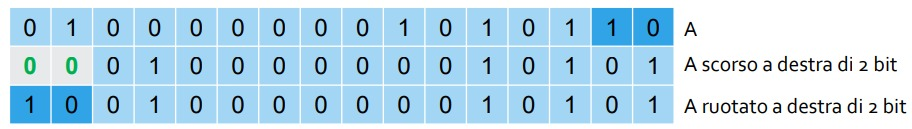
\includegraphics[width=0.85\textwidth]{SHIFT_ROTAZIONE}
			\end{figure}
			La rotazione è utile per l'impacchettamento di sequenza di bit in parole e per il loro spacchettamento. Se si vuole esaminare una parola bit per bit, la si può rotare di 1 bit alla volta ed esaminare ogni volta il bit di segno, dopo aver esaminato tutti i bit la parola ritorna nella sua forma originale.
			\item le \textbf{operazioni binarie} che producono un risultato dalla combinazione dei due operandi e tra queste operazioni ci sono anche le operazioni booleane come \textbf{AND, OR e NOT} e a volte si trovano anche \textbf{XOR, NOR e NAND}. Tutte queste operazioni sono \textbf{\textit{bitwise}}, cioè effettuano il calcolo bit a bit. 
		\end{itemize}
		Un uso importante dell'AND è l'\textbf{\textbf{estrazione della parola}}. Questo avviene tramite l'utilizzo di un AND tra il dato originale e una costante, la \textbf{maschera}, che identifica la parola da estrarre. La maschera è composta da 1 dove ci sono i bit da estrarre e di 0 negli altri bit:
		\begin{figure}[H]
			\centering
			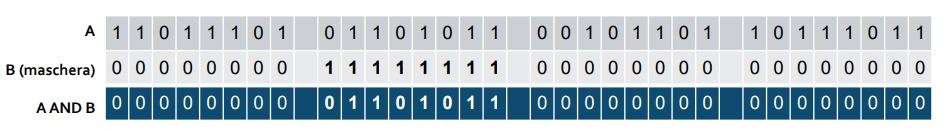
\includegraphics[width=1.0\textwidth]{ESTRAZIONE_AND}
		\end{figure} 
		Il risultato viene fatto scorrere di 16 bit verso destra in modo da isolare il carattere da estrarre all'estremità destra della parola.\\
		L'OR, invece, viene usato per \textbf{\textit{impacchettare bit in una parola}}:
		\begin{figure}[H]
			\centering
			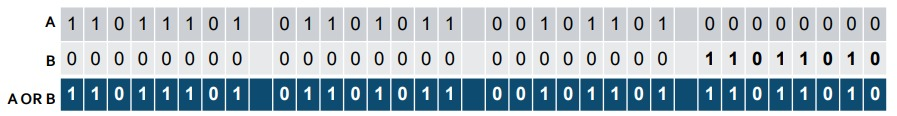
\includegraphics[width=1.0\textwidth]{IMPACCHETTAMENTO_OR}
		\end{figure}
		Per \textbf{\textit{sostituire una parola}}, invece, si utilizza in sequenza l'estrazione e l'impacchettamento:
		\begin{figure}[H]
			\centering
			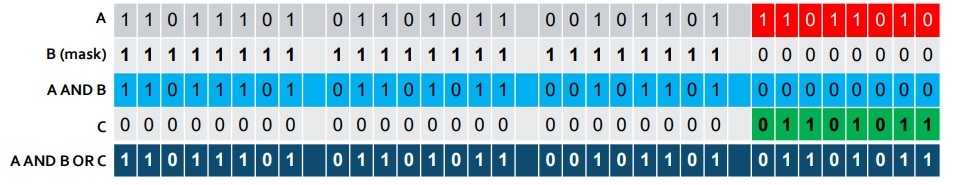
\includegraphics[width=1.0\textwidth]{SOSTITUZIONE_AND_OR}
		\end{figure}
		Esistono altri tipologie di istruzioni, quali:
		\begin{itemize}
			\item \textbf{istruzioni di confronto}: come l'uguaglianza tra parole, verificare se una parola è 0 o il confronto di maggioranza o minoranza tra numeri
			\item \textbf{istruzioni di I/O}: sono quelle che interagiscono con i dispositivi di I/O e sono di tre tipi:
			\begin{itemize}
				\item I/O \textbf{programmato con attesa attiva} impiegato nei sistemi di fascia bassa come i sistemi integrati o quelli che devono rispondere subito agli stimoli esterni. Queste CPU di solito hanno una sola istruzione di input e una di output che trasferisce un carattere per volta da un registro prefissato al dispositivo I/O prescelto. \\
				Per ogni carattere la CPU deve aspettare che il dispositivo I/O sia pronto prima di poterlo ottenere e quindi la CPU passa gran parte del tempo ad aspettare che il dispositivo sia pronto, per questo si parla di \textbf{attesa attiva} ed è accettabile se la CPU non ha altro da eseguire.
				\item I/O \textbf{interrupt driven}, che viene innescato dagli interrupt, dove la CPU fa partire il dispositivo di I/O e gli impartisce l'ordine di generare un interrupt quando ha finito, quindi l'operazione di I/O termina tramite l'asserzione del bit \textbf{INTERRUPT ABILITATO}. \\
				Anche se questo è un gran progresso rispetto all'I/O programmato non è perfetto perchè ci vuole un interrupt per ogni carattere trasferito e l'elaborazione di un interrupt è gravosa.
				\item I/O \textbf{con DMA}, cioè l'I/O programmato ma viene aggiunto il chip \textbf{\textit{Direct Memory Access}} che ha accesso diretto al bus. Questo chip ha 4 registri accessibili dal software in esecuzione: il primo contiene l'indirizzo di memoria per la lettura o scrittura; il seconda conta il numero di byte da trasferire; il terzo specifica il numero del dispositivo o lo spazio d'indirizzamento I/O da usare; il quarto determina se i dati devono essere letti dal dispositivo o se vanno scritti su di esso. \\
				Anche se il DMA toglie il carico pesante dell'I/O il procedimento non è gratuito, perchè se ad esempio un disco ad alta velocità è in fase di trasferimento ci vorranno molti cicli di bus per l'accesso alla memoria e al dispositivo e durante questo periodo la CPU deve rimanere in attesa. Questo fenomeno si chiama \textbf{appropriazione di cicli} quando la DMA sottrae cicli di bus alla CPU.
			\end{itemize}
			\item \textbf{istruzioni di salto (JUMP)}: il codice viene scritto mediante l'ausilio di etichette che definiscono delle sezioni del programma e queste istruzioni consentono al programma di passare da una sezione all'altra, i salti possono essere di diverse tipologie, quali:
			\begin{itemize}
				\item \textbf{salti incondizionati}: (GOTO) si passa direttamente ad un'altra sezione del programma
				\item \textbf{Salti condizionati}: si passa ad un'altra sezione del programma a seconda del risultato della condizione data
			\end{itemize}
			(Vedere pdf per esempio dei "spaghetti code")
			\item \textbf{istruzioni di ciclo}: vengono convertite in salti condizionati, in quanto le istruzioni di ciclo prevedono un contatore che incrementa o decrementa a ogni iterazione del ciclo, questo contatore viene esaminato a ogni iterazione e il ciclo termina quando si verifica una determinata condizione.
			\item \textbf{Invocazione di procedura}: Una procedura è un'insieme di istruzioni che svolge un certo compito e che può essere invocata da diversi punti di un rpogramma. Quando una procedura ha terminato il proprio compito l'esecuzione deve riprendere dall'istruzione successiva alla chiamata. A tal fine l'indirizzo di ritorno deve essere passato alla procedura o salvato da qualche parte dove possa essere recuperato al momento del ritorno. \\
			L'indirizzo di ritorno può essere salvato in tre posti diversi: in memoria, in un registro o nello stack. La soluzione peggiore è salvarlo in una locazione di memoria fissa perchè se la procedura chiama un'altra procedura, la seconda chiamata causerebbe la perdita dell'indirizzo di ritorno della prima. \\
			Una soluzione un tantino migliore consiste nel far si che l'istruzione di chiamata di procedura salvi l'indirizzo di ritorno nella prima parola della procedura. In questo modo la procedura potrebbe richiamare altre procedure, visto che ciascuna alloca lo spazio per il proprio indirizzo di ritorno. Questo schema è fallimentare se la procedura è ricorsiva perchè l'indirizzo di ritorno verrebbe cancellato dalla seconda chiamata. \\
			La soluzione migliore si ottiene se l'istruzione di chiamata di procedura pone l'indirizzo di ritorno in un registro, affidando alla procedura la responsabilità di salvarlo in un posto sicuro. Se la procedura è ricorsiva, la procedura è ricorsiva la procedura dovrà preoccuparsi di salvare l'indirizzo di ritorno in un posto differente ogni volta che viene invocata. \\
			La cosa migliore che può fare l'istruzione di chiamata di procedura è porre l'indirizzo di ritorno in cima a uno stack. Quando la procedura termina fa un pop dell'indirizzo di ritorno e lo scrive nel program counter. Questo meccanismo prende il nome di \textbf{stack di attivazione} o \textbf{record di attivazione}.
			\begin{figure}[H]
				\centering
				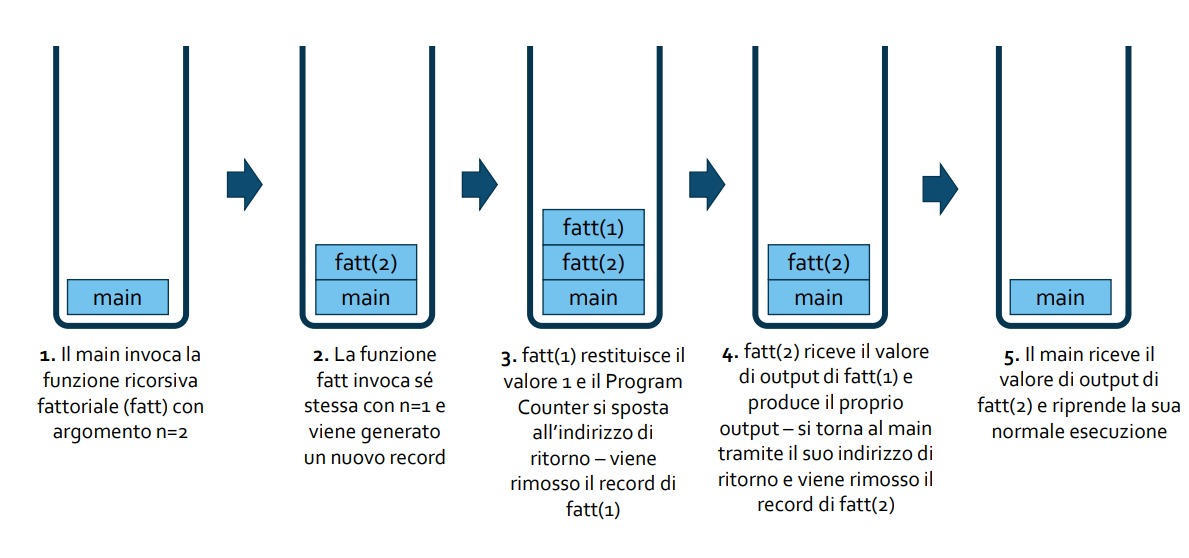
\includegraphics[width=0.75\textwidth]{STACK_ATTIVAZIONE}
			\end{figure}
		\end{itemize}
		\section{Formato delle istruzioni}
		Le istruzioni sono composte da:
		\begin{itemize}
			\item un \textbf{codice operativo}, l'\textbf{OPCODE};
			\item altre informazioni come la provenienza degli operandi e la destinazione dei risultati.
		\end{itemize}
		Quando parliamo di provenienza degli operandi, intendiamo il loro \textbf{indirizzo} e come vedremo ci sono diverse tipologie di indirizzamento possibili. \\
		Un'istruzione è dotata quindi di un opcode che ne specifica il comportamento e può contenere nessuno, uno, due o tre indirizzi o operandi. Segue un esempio di alcune possibili istruzioni con o senza operandi:
		\begin{figure}[H]
			\centering
			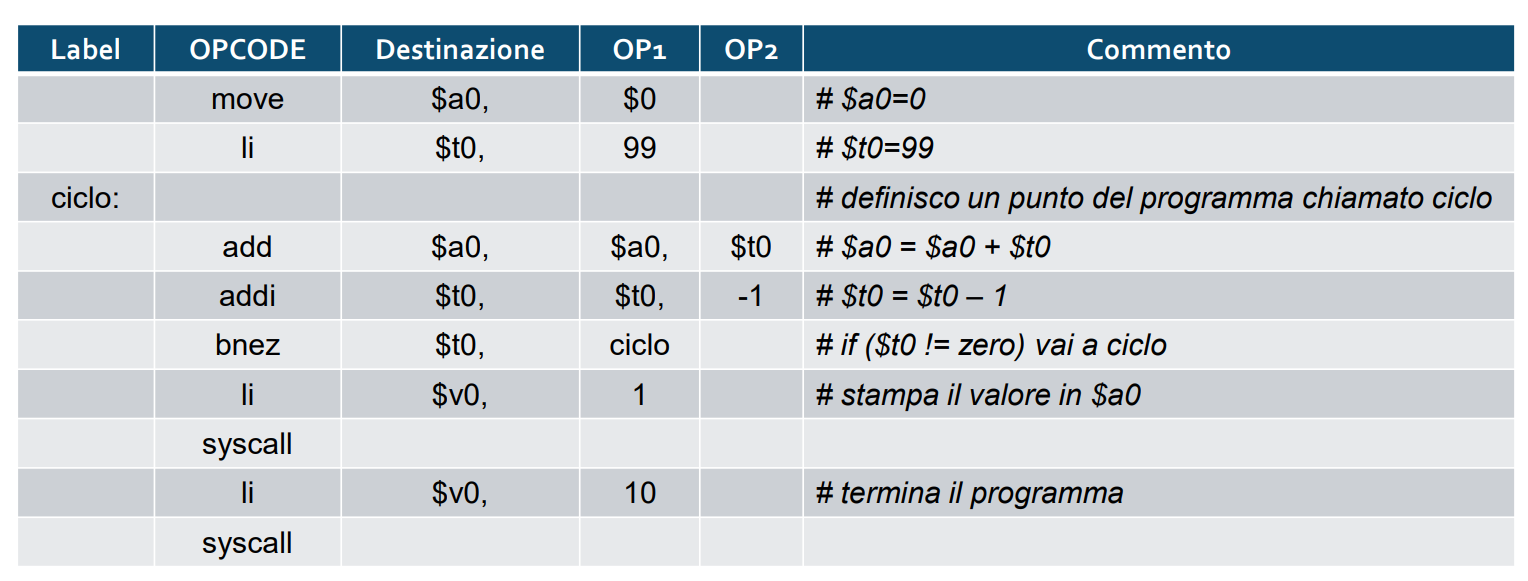
\includegraphics[width=1.00\textwidth]{Assembly_instructions}
		\end{figure}
		I progettisti di computer durante la fase di progettazione devono scegliere il formato delle istruzioni, ed è una scelta importante che non va sottovalutata. \\
		Una capacità importante è quella di saper aggiungere nuove istruzioni per far fronte alle nuove esigenze che si riscontrano con il passare degli anni, evitando, però, che questa aggiunta non vada a rendere i vecchi programmi incompatibili con il modello precedentemente creato e quindi l'obiettivo è quello di rendere l'ISA retrocompatibile, caratteristica già affrontata precedentemente. \\
		A parità di progetto, le istruzioni corte sono preferibili alle istruzioni lunghe, perchè un programma con \textit{n} istruzioni di 16 bit occupa metà spazio di memoria di un programma con \textit{n} istruzioni a 32 bit, anche se ormai questo fattore potrebbe risultare sempre meno importante in futuro in quanto il costo della memoria diminuisce sempre di più, anche se le dimensioni del software hanno un aumento più veloce rispetto alla diminuzione del costo della memoria. Inoltre, minimizzare la dimensione delle istruzioni richiederebbe più tempo per decodificarle e quindi se si vuole avere delle istruzioni minime si deve valutare il tempo richiesto per la loro decodifica ed esecuzione. \\
		Un'altra ragione importante per minimizzare la dimensione delle istruzioni, e che diventerà sempre più importante al crescere delle prestazioni del processore è legata all'ampiezza di banda della memoria, cioè quanti bit può trasferire in un secondo. \\
		Inoltre, bisogna prevedere nel formato delle istruzioni spazio sufficiente a esprimere tutte le operazioni volute. Se desideriamo avere $2^n$ possibili operazioni differenti, dobbiamo rappresentarle con \textbf{\textit{almeno}} $n$ bit destinati all'OPCODE.
		Bisogna sottolineare che devono essere \textbf{\textit{almeno}} $n$ bit perchè, supponendo di voler avere 16 operazioni differenti, abbiamo bisogno di 4 bit per rappresentarle, ma, possiamo anche scegliere di destinare, ad esempio, 5 bit all'OPCODE così se in futuro volessimo rappresentare ulteriori operazioni, non abbiamo bisogno di modificare il formato delle istruzioni perchè è abbiamo già destinato precedentemente ulteriori bit all'OPCODE e quindi in questo modo abbiamo reso \textit{\textbf{retrocompatibile}}.\\
		Un terzo criterio è la \textbf{scelta della dimensione degli indirizzi} che dipende dalla dimensione delle parole in memoria, quindi:
		\[
		n_{indirizzi} = \dfrac{dimensione_{memoria}}{dimensione_{parola}} \\
		\]
		\[
		dimensione\_indirizzo = \lceil \log_2 (n_{indirizzi}) \rceil
		\]
		\textbf{Nota:} Si esegue il logaritmo in base 2 perchè se abbiamo un $x$ numero di indirizzi disponibili, allora per conoscere la dimensione in bit di un singolo indirizzo bisogna fare il logaritmo, infatti $2^{dimensione_indirizzo}$ ci da esattamente il numero di indirizzi disponibili. \\
		Scegliere la dimensione delle parole di più o meno bit comporta vantaggi e svantaggi, è bene comunque ricordare che indirizzi più corti consentono istruzioni più corte, che occuperebbero meno spazio e richiederebbero meno tempo in fase di fetch.
		\section{Codice operativo estendibile}
		Si consideri un'istruzione lunga $(n + k)$ bit dove $n$ è il numero di bit destinati all'OPCODE mentre $k$ è il numero di bit destinati a un solo operando, in questo modo abbiamo:
		\begin{itemize}
			\item $2^n$ istruzioni possibili differenti
			\item $2^k$ celle di memoria indirizzabili
		\end{itemize}
		Questi $(n + k)$ bit possono essere spezzati in $(n - 1)$ bit di OPCODE e $(k + 1)$ bit d'indirizzo, in questo modo stiamo dimezzando il numero di operazioni possibili e stiamo raddoppiando il numero d'indirizzi di memoria disponibili. \\
		In alternativa, possiamo spezzare questi $(n + k)$ bit in $(n + 1)$ bit di OPCODE e $(k - 1)$ bit d'indirizzo, così facendo stiamo raddoppiando il numero di operazioni possibili e stiamo dimezzando il numero d'indirizzi di memoria disponibili. \\
		Dopo questo breve esempio, si può introdurre il concetto di \textbf{\textit{codice operativo estensibile}}. \\
		Supponiamo di avere una macchina le cui istruzioni sono lunghe 16 bit, destinando 4 bit all'OPCODE e 4 bit per singolo indirizzo, pertanto otteniamo: 
		\begin{figure}[H]
			\centering
			\includegraphics[width=1.00\textwidth]{Codice_OP_Estensibile}
		\end{figure}
		In questo modo possiamo rappresentare $2^4$ istruzioni differenti che operando con tre indirizzi in memoria. \\
		Se desideriamo aumentare il lotto di istruzioni, possiamo espandere l'OPCODE utilizzando i bit degli operandi, senza aggiungere ulteriori bit che comporterebbero uno spreco. \\
		Quindi possiamo riservare delle configurazioni nei bit destinati all'OPCODE. Ad esempio, se riserviamo la configurazione 1111 nei bit destinati all'OPCODE, indichiamo che l'istruzione è nel formato OPCODE + 2 operandi e di fatti i bit dell'OPCODE passano a 8 e sono 1111xxxx, in questo modo otteniamo:
		\begin{itemize}
			\item $2^4 - 1$ istruzioni a tre indirizzi di memoria +
			\item $2^4$ istruzioni con due operandi
		\end{itemize}
		Questo meccanismo lo possiamo anche continuare ad applicare per le istruzioni a un operando e senza operandi e otterremmo:
		\begin{figure}[H]
			\centering
			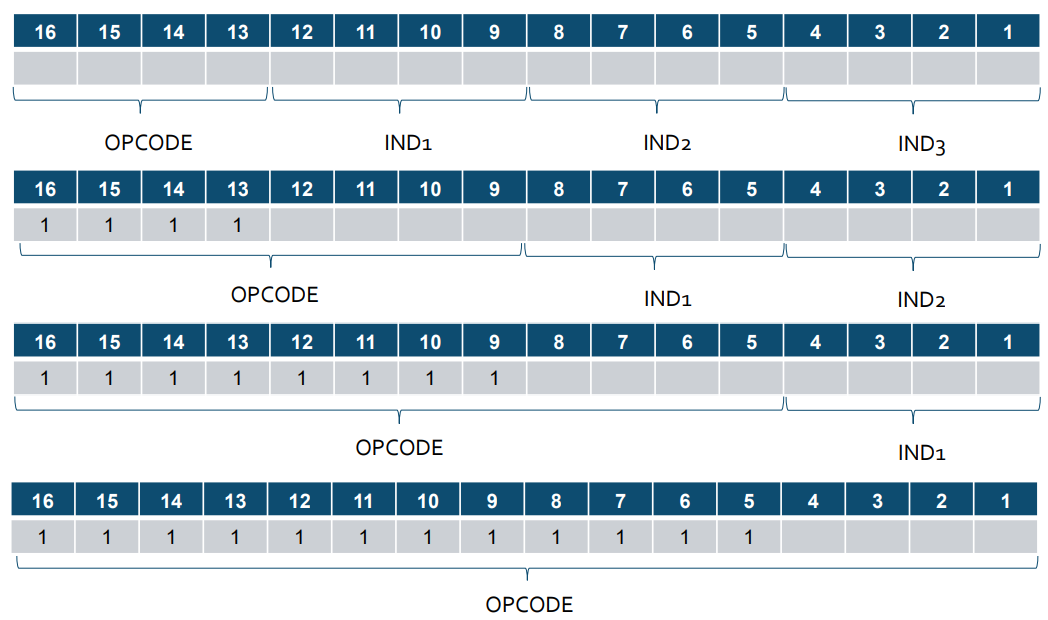
\includegraphics[width=1.00\textwidth]{Codice_estensibile_esempio}
		\end{figure}
		La tecnica del codice operativo estensibile descritta sopra, è solo un esempio, infatti la si può gestire in qualsiasi maniera differente in base alle proprie esigenze, infatti se si desidera, ad esempio, avere più istruzioni a 2 operandi e meno a 3 operandi è possibile avere un set di $2^4 - 2$ istruzioni disponibili a 3 operandi, dove il -2 sono le configurazioni 1110 e 1111 e $2^5$ istruzioni disponili a 2 operandi, ottenendo lo schema seguente:
		\begin{figure}[H]
			\centering
			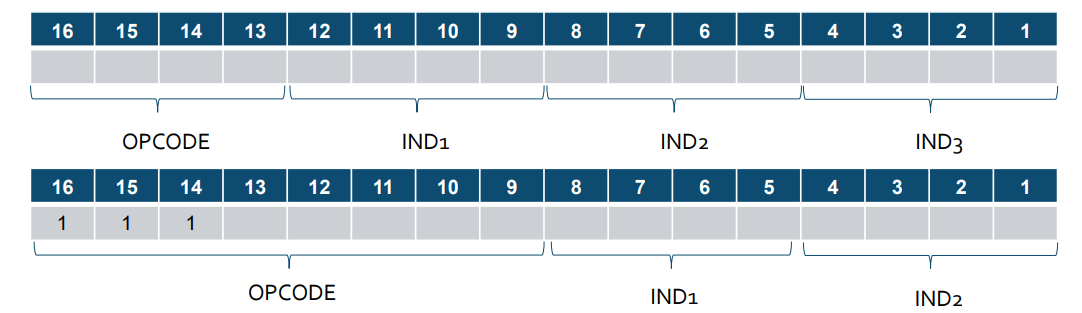
\includegraphics[width=1.00\textwidth]{Codice_estensibile_esempio2}
		\end{figure}
		\section{Indirizzamento}
		Molte istruzioni, come abbiamo detto, contengono operandi e il problema è come specificarne la posizione. Ci sono diverse tipologie d'indirizzamento e sono:
		\begin{itemize}
			\item Immediato;
			\item Diretto;
			\item A registro;
			\item A registro indiretto;
			\item Indicizzato;
			\item Indicizzato esteso;
			\item A stack.
		\end{itemize}
		\subsection{Indirizzamento immediato}
		L'indirizzamento immediato è il modo più semplice con cui un'istruzione può specificare un operando, ed è quello di contenere nel campo riservato al suo indirizzo, l'operando stesso invece che il suo indirizzo. Un operando così specificato si dice \textbf{immediato} perchè viene recuperato dalla memoria nel momento stesso in cui viene effettuato il fetch dell'istruzione. Un esempio di istruzione con indirizzamento immediato è: MOV R1 4, che carica la costante 4 nel registro R1.  \\
		Il vantaggio è quello di non richiedere un riferimento supplementare in memoria per il fetch dell'operando però lo svantaggio è quello di poter fornire solo un operando per volta e l'entità del valore è limitata alla dimensione del campo, quindi questa tecnica è adatta per la specifica di piccole costanti intere.
		\subsection{Indirizzamento diretto}
		Un metodo per specificare un operando in memoria è darne l'indirizzo completo. Come l'indirizzamento immediato, l'indirizzamento diretto presenta dei limiti perchè l'istruzione accederà sempre alla stessa locazione di memoria, quindi se da una parte il contenuto può cambiare la locazione no. Per questo l'indirizzamento diretto serve solo ad accedere a variabili globali il cui indirizzo è noto in fase di compilazione e non può essere un indirizzo contenuto all'interno di una procedura, in quanto l'allocazione avverrebbe durante l'invocazione della funzione stessa.
		\subsection{Indirizzamento a registro}
		L'indirizzamento a registro ha un funzionamento analogo all'indirizzamento diretto, ma specifica un registro invece di una locazione di memoria, questa è la modalità d'indirizzamento più usata dato che i registri sono veloci in accesso e hanno indirizzi brevi.
		Nelle architetture load/store, ovvero le architetture dove si può operare solo tramite operandi su registri, tutte le istruzioni utilizzano questa modalità, a meno delle istruzioni LOAD e STORE che caricano/scaricano dati in memoria da/verso un registro. 
		\subsection{Indirizzamento a registro indiretto}
		In questa modalità, l'operando proviene o è destinato alla memoria, ma il suo indirizzo non è incorporato nell'istruzione perchè l'indirizzo è contenuto in un registro, questo prende il nome di \textbf{puntatore}. Il vantaggio è proprio la capacità di referenziare la memoria senza che l'indirizzo di memoria sia incorporato all'interno dell'istruzione stessa, inoltre la stessa istruzione può essere utilizzata su diverse parole in memoria, semplicemente variando il valore contenuto nel registro.
		\subsection{Indirizzamento indicizzato}
		Questa modalità d'indirizzamento consente di referenziare una parola di memoria che si trova a un certo spiazzamento rispetto a un registro.
		L'indirizzamento alla memoria si ottiene specificando un registro, in maniera esplicita o implicita più uno spiazzamento costante. Questo meccanismo viene utilizzato in alcune occasioni nelle quali è nota a priori la distanza tra una variabile e l'altra ed è anche possibile la soluzione opposta, cioè tenere il puntatore alla memoria dell'istruzione e il piccolo offset in un registro. \\
		Vedere gli esempi dal libro.
		\subsection{Indirizzamento indicizzato esteso}
		L'indirizzamento indicizzato esteso consente di referenziare una parola di memoria ottenuto sommando tra loro il contenuto di due registri più un offset opzionale. Un registro funge da base e l'altro da indice, molto utile nel caso in cui si scrive in linguaggio macchina un ciclo che opera su un vettore. \\
		Generalmente le macchine che offrono questa possibilità forniscono anche un offset da 8 o 16 bit.
		\subsection{Indirizzamento a stack}
		Come precedentemente detto, è consigliabile rendere le istruzioni macchina il più corte possibile. Il limite alla riduzione degli indirizzi equivale a non averne per nulla, come l'istruzione IADD e queste istruzioni sono possibili in associazione con uno stack.\\
		Uno degli esempi pratici di utilizzo è legato alla \textbf{\textit{notazione polacca inversa}}.
		\subsection{Notazione polacca inversa}
		Solitamente scriviamo le operazioni algebriche utilizzando la \textbf{notazione infissa}, cioè quando l'operatore è posto tra gli operandi, cioè: 
		\[
		A + B
		\]
		ed esistono anche la notazione prefissa e postfissa, che sono rispettivamente: $+AB$ e $AB+$. \\
		La notazione postfissa prende anche il nome di \textbf{\textit{notazione polacca inversa}} dal logico polacco Lukasiewicz che ne studiò le proprietà. \\
		Questa notazione presenta diversi vantaggi, come:
		\begin{itemize}
			\item ogni operazione può essere scritta correttamente senza parentesi;
			\item la valutazione delle formule in tale notazione si addice particolarmente ai compilatori con stack;
			\item gli operatori infissi inoltre, possiedono un ordine di precedenza, che è arbitrario, infatti $a + b \times c$ equivale a $a + (b \times c)$ e non a $(a + b) \times c$, perchè la moltiplicazione ha un ordine di priorità più alto.
			\textbf{Nota:} L'ordine delle variabili	è lo stesso nelle due notazioni, mentre l'ordine degli operandi può cambiare. Nella notazione polacca inversa, l'ordine degli operatori compaiono nell'ordine in cui verranno effettivamente eseguiti.
		\end{itemize}
		Seguono alcuni esempi di notazione polacca inversa:
		\begin{center}
			\begin{tabular}{c | c}
				\textbf{Notazione infissa} & \textbf{Notazione polacca inversa} \\
				\hline
				$A \times B + C$ & $AB\times C + $ \\
				\hline
				$A + B \times C$ & $ABC\times +$ \\
				\hline
				$A \times B + C \times D$ & $AB\times CD \times +$ \\
				\hline
				$((A + B) \times C + D) / (E + F + G)$ & $AB+C\times D+ EF+G+ /$
			\end{tabular}
		\end{center}
		Per valutare una formula in notazione polacca inversa, quando trovo un valore lo aggiungo in cima allo stack, quando trovo un operando prendo i due valori in cima allo stack, effettuo l'operazione tra questi due e inserisco il risultato in cima allo stack.\\
		Segue un esempio più complesso, data l'espressione $(8+2\times5)/(1+3\times2-4)$: 
		\begin{figure}[H]
			\centering
			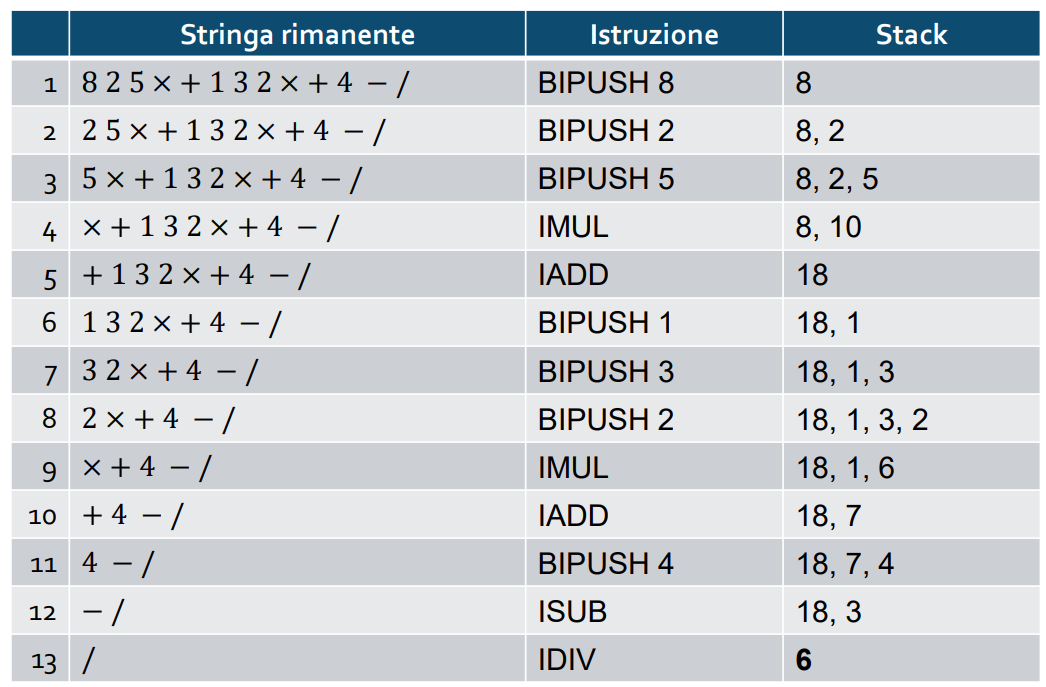
\includegraphics[width=1.00\textwidth]{Notazione_polacca_inversa}
		\end{figure}
		Per passare dalla notazione infissa alla notazione polacca inversa si usa l'\textbf{\textit{algoritmo di scala di manovra}}, lo \textit{Shunting-yard algorithm}, detto anche \textit{algoritmo di smistamento}, inventato da Edsger Dijkstra. \\
		L'algoritmo consiste nell'analizzare l'espressione e trasferire gli operatori in uno stack apposito, che selezione se inserire l'operatore o tenerlo in memoria sulla base della prorità dell'operazione:
		\begin{figure}[H]
			\centering
			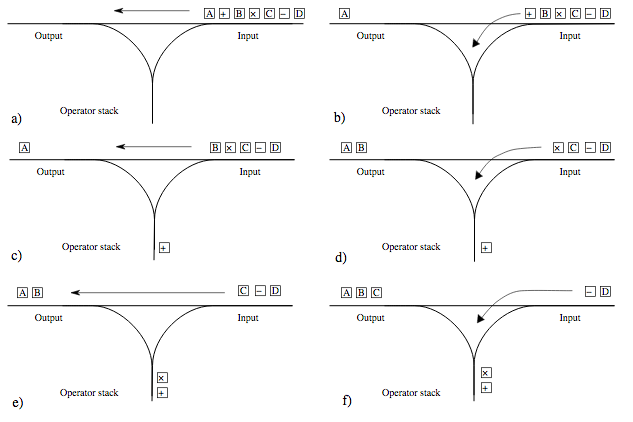
\includegraphics[width=0.70\textwidth]{Shunting_yard}
		\end{figure}
		\subsection{Modalità di indirizzamento per le istruzioni di salto}
		Anche le istruzioni di salto e le chiamate di procedura necessitano di modalità di indirizzamento per specificare l'indirizzo di destinazione. Le modalità analizzate finora funzionano grosso modo anche per i salti. L'indirizzamento diretto è di un'operazione possibile. Un'altra possibilità è effettuare l'indirizzamento a registro indiretto che consente al programma di calcolare l'indirizzo di destinazione, scriverlo in un registro ed effettuare il salto. Un'altra modalità ragionevole è la modalità indicizzata, che specifica un certo offset rispetto all'indirizzo contenuto in registro.
		\section{Controllo del flusso}
		Il controllo del flusso riguarda la sequenza con cui le istruzioni vengono eseguite dinamicamente. In mancanza d'istruzioni di salto o di chiamata di procedura, le istruzioni vengono eseguite nello stesso ordine con cui si susseguono in memoria. Le chiamate di procedura alterano il controllo del flusso perchè arrestano la procedura correntemente in esecuzione e cominciano l'esecuzione della procedura chiamata. Anche le trap e gli interrupt provocano un'alterazione del flusso esecutivo quando si verificano delle condizioni speciali. \\
		Dopo l'esecuzione di un'istruzione, viene recuperata ed eseguita l'istruzione che la segue in memoria. Al termina di ciascuna istruzione, il PC viene incrementato della lunghezza dell'istruzione elaborata. Il PC è una funzione lineare nella variabile tempo e che aumenta in ogni unità di tempo, di una quantità pari alla lunghezza media delle istruzioni diviso il loro tempo medio di esecuzione. In presenza di salti, però, il PC non è più una funzione monotona crescente nel tempo.
		\subsection{Procedure}
		Le procedure costituiscono la tecnica più importante per la strutturazione dei programmi. Da un certo punto di vista una chiamata di procedura altera il flusso esecutivo tanto quanto un salto, ma alla terminazione del suo compito la procedura ripassa il controllo al comando o all'istruzione che segue la sua chiamata. \\
		Una tipologia di procedure particolarmente importanti è quella delle \textbf{procedure ricorsive}, ovvero le procedure che richiamano se stesse. Al fine di poter gestire le procedure ricorsive abbiamo bisogno di uno stack per memorizzare i parametri e le variabili locali a ogni invocazioni. Ogni volta che una procedura viene chiamata, in cima allo stack viene allocato un record d'attivazione per la procedura stessa. Oltre al puntatore allo stack, che punta alla cima della pila, risulta conveniente avere un puntatore al record d'attivazione, FP o Frame Pointer, che punta ad una locazione nota del record d'attivazione. Le prime cose che una procedura invocata deve fare sono il salvataggio del vecchio FP, la copia di SP in FP e l'eventuale incremento di FP di una parola, a seconda della locazione cui puntare nel nuovo record d'attivazione. \\
		Il punto chiave è poter effettuare un ritorno da procedura e ripristinare lo stato dello stack alla situazione in cui si trovava appena prima dell'invocazione della procedura. Il codice che si occupa di salvare il vecchio FP e aggiornarlo è detto \textbf{prologo della procedura}. All'uscita della procedura si rende invece necessario ripulire lo stack, che rappresenta la fase di \textbf{epilogo della procedura}.
		\section{Coroutine}
		\section{Trap}
		Una \textbf{trap} è una specie di chiamata di procedura automatica effettuata quando si verificano certe condizioni causate da un programma e che sono in genere eventi rilevanti. Un buon esempio è l'overflow: in molti computer se il risultato di un'operazione aritmetica eccede il più grande numero rappresentabile si verifica una trap, ovvero il controllo del flusso viene interrotto e riprende da una locazione di memoria prefissata all'interno della quale si trova l'indirizzo per un salto a una procedura detta \textbf{gestore di trap} che svolge le operazioni appropriate. \\
		Alcune delle condizioni che causano comunemente trap sono gli overflow e gli underflow, le violazioni di protezione, gli opcode non definiti, gli overflow di stack, i tentativi di utilizzare dispositivi di I/O inesistenti, i tentativi di fetch di una parola da un indirizz dispari, la divisione per zero.
		\subsection{Interrupt}
		Gli \textbf{interrupt} sono cambiamenti del flusso esecutivo causati non dal programma in esecuzione, ma da qualche altro problema, generalmente determinato dall'I/O. \\
		Per esempio un programma potrebbe ordinare al disco di iniziare il trasferimento delle informazioni e di inviare un interrupt non appena il trasferimento termini. Gli interrupt interrompono il programma in esecuzione e trasferiscono il controllo a un gestore deputato a svolgere le azioni appropriate. Al loro compimento, il gestore di interrupt restituisce il controllo al programma interrotto ed è suo compito far riprendere il processo interrotto esattamente dallo stesso stato in cui si trovata al momento dell'interruzione. \\
		La differenza tra le trap e gli interrupt è che le trap sono sincrone al programma e gli interrupt sono asincroni. Se un programma viene rieseguito tante volte con lo stesso input, le trap si verificheranno sempre nello stesso punto, mentre gli interrupt possono variare a seconda, ad esempio, di quando viene premuto il tasto d'invio dal terminale. Le trap, quindi, sono causate direttamente dal programma, gli interrupt, sono causati dal programma per lo più indirettamente. \\
		Un concetto chiave di interrput è la \textbf{trasparenza}. Al verificarsi di un interrupt si intraprendono alcune azioni e si procede con l'esecuzione di un certo codice, ma quando tutto è finito il computer deve ripartire dallo stato che aveva prima dell'interrupt. \\
		Inoltre, un calcolatore presenta diversi dispositivi di I/O e può capitare che più dispositivi nello stesso istante vogliano generare un interrupt. Ci sono due strategie per affrontare questo problema. La prima è far si che ogni routine di interrupt disabiliti eventuali interrupt successivi e questo approccio gestisce gli interrupt in maniera sequenziale. \\
		Alternativamente, una migliore strategia consiste nell'assegnare una priorità ad ogni dispositivo di I/O: alta per i dispositivi per i quali la gestione del tempo è critica, bassa per gli altri. \\
		Durante l'esecuzione di una routine di interrupt di priorità \textit{n}, ognii tentativo di interruzione di dispositivi con priorità minore viene ignorato finchè la routine attuale non viene completata. \\
		A partire dall'8088, tutte le CPU Intel sono state dotate di due livelli di interrupt: mascherabile e non mascherabile. Gli interrupt non mascherabili sono usati per segnalare eventi catastrofici e i dispositivi di I/O usano interrupt mascherabili. \\
		Per i dispositivi di I/O, essendoci un solo livello di interrupt utilizzabile, la CPU non ha modo di far si che un dispositivo di priorità maggiore interrompa una routine di servizio di priorità inferiore. Per risolvere questo problema le CPU Intel sono spesso usate in congiunzione con un controllore esterno di interrupt.
		\chapter{Esercizi di algebra Booleana}
		\begin{enumerate}
			\item $F = \overline{\overline{A} * B} \oplus \overline{C + A} + $
			\\ \textbf{Tabella di verità: }
			\\ 
			\\
			\begin{tabular}{c|c|c|c|c|c|c|c|c}
				A & B & C & $\overline{A}$ & $\overline{A} * B$& $\overline{\overline{A} * B}$& C + A & $\overline{C + A}$ & $ \overline{\overline{A} * B} \oplus \overline{C + A}$ \\
				\hline
				0 & 0 & 0 & 1 & 0 & 1 & 0 & 1 & 0 \\
				0 & 0 & 1 & 1 & 0 & 1 & 1 & 0 & 1 \\
				0 & 1 & 0 & 1 & 1 & 0 & 0 & 1 & 1 \\
				0 & 1 & 1 & 1 & 1 & 0 & 1 & 0 & 0 \\
				1 & 0 & 0 & 0 & 0 & 1 & 1 & 0 & 1 \\
				1 & 0 & 1 & 0 & 0 & 1 & 1 & 0 & 1 \\
				1 & 1 & 0 & 0 & 0 & 1 & 1 & 0 & 1 \\
				1 & 1 & 1 & 0 & 0 & 1 & 1 & 0 & 1 \\
			\end{tabular}
			\\ Fare il circuito logico
			\item $F = A \ \oplus \ \overline{B} * A \ \oplus \ C$
			\\ \textbf{Tabella di verità: }
			\\ Fare tabella. ricordare che il prodotto logico ha precedenza sugli xor. Le precedenze sono NOT, AND, OR, XOR
			\\ \textbf{Circuito logico, anche qui rispettare le precedenze}
			\item $F = \overline{A * \overline{\overline{B} + C} \ \oplus \ D}$
			\\ Fare tabella di verità
			\\ Fare circuito logico
			\item $F = \overline{A \ \oplus \ B} * A + C \ \oplus \ B $
		\end{enumerate}
\end{document}
